\documentclass[11pt,twoside]{report}
\usepackage{hyperref}
\usepackage{graphicx}
\usepackage{amsmath, amssymb}
\usepackage[table]{xcolor}
\usepackage[toc,page]{appendix}
\usepackage{amssymb}
\usepackage{csquotes}
\usepackage{amsthm}
\usepackage{subdepth}
\usepackage{algorithm}
\usepackage[noend]{algpseudocode}
\usepackage{wrapfig}
\usepackage{enumitem}
\usepackage{listings}
\usepackage{color}
\usepackage{xcolor}
% \usepackage{minted}

\usepackage{algpseudocode}
\algrenewcommand\algorithmicrequire{\textbf{Input:}}

\usepackage[noend]{algpseudocode}

\makeatletter
\def\BState{\State\hskip-\ALG@thistlm}
\makeatother

\makeatletter
\algnewcommand{\LineComment}[1]{\Statex \hskip\ALG@thistlm \(\triangleright\) #1}
\makeatother

\definecolor{codegray}{rgb}{0.8,0.8,0.8}
\definecolor{codepurple}{rgb}{0.58,0,0.82}
\definecolor{backcolour}{rgb}{0.95,0.95,0.92}


% \usepackage[top=1in]{geometry}
\usepackage{textcomp}
\usepackage{listings}
%\usepackage{minted}      % (requires -shell-escape)
\usepackage{xcolor}
\usepackage{filecontents}

% --- ugly internals for language definition ---
%
\makeatletter

% initialisation of user macros
\newcommand\PrologPredicateStyle{}
\newcommand\PrologVarStyle{}
\newcommand\PrologAnonymVarStyle{}
\newcommand\PrologAtomStyle{}
\newcommand\PrologOtherStyle{}
\newcommand\PrologCommentStyle{}

% useful switches (to keep track of context)
\newif\ifpredicate@prolog@
\newif\ifwithinparens@prolog@

% save definition of underscore for test
\lst@SaveOutputDef{`_}\underscore@prolog

% local variables
\newcount\currentchar@prolog


\newcommand\@testChar@prolog%
{%
  % if we're in processing mode...
  \ifnum\lst@mode=\lst@Pmode%
    \detectTypeAndHighlight@prolog%
  \else
    % ... or within parentheses
    \ifwithinparens@prolog@%
      \detectTypeAndHighlight@prolog%
    \fi
  \fi
  % Some housekeeping...
  \global\predicate@prolog@false%
}



% helper macros
\newcommand\detectTypeAndHighlight@prolog
{%
  % First, assume that we have an atom.
  \def\lst@thestyle{\PrologAtomStyle}%
  % Test whether we have a predicate and modify the style accordingly.
  \ifpredicate@prolog@%
    \def\lst@thestyle{\PrologPredicateStyle}%
  \else
    % Test whether we have a predicate and modify the style accordingly.
    \expandafter\splitfirstchar@prolog\expandafter{\the\lst@token}%
    % Check whether the identifier starts by an underscore.
    \expandafter\ifx\@testChar@prolog\underscore@prolog%
      % Check whether the identifier is '_' (anonymous variable)
      \ifnum\lst@length=1%
        \let\lst@thestyle\PrologAnonymVarStyle%
      \else
        \let\lst@thestyle\PrologVarStyle%
      \fi
    \else
      % Check whether the identifier starts by a capital letter.
      \currentchar@prolog=65
      \loop
        \expandafter\ifnum\expandafter`\@testChar@prolog=\currentchar@prolog%
          \let\lst@thestyle\PrologVarStyle%
          \let\iterate\relax
        \fi
        \advance \currentchar@prolog by 1
        \unless\ifnum\currentchar@prolog>90
      \repeat
    \fi
  \fi
}

\newcommand\splitfirstchar@prolog{}
\def\splitfirstchar@prolog#1{\@splitfirstchar@prolog#1\relax}
\newcommand\@splitfirstchar@prolog{}
\def\@splitfirstchar@prolog#1#2\relax{\def\@testChar@prolog{#1}}

% helper macro for () delimiters
\def\beginlstdelim#1#2%
{%
  \def\endlstdelim{\PrologOtherStyle #2\egroup}%
  {\PrologOtherStyle #1}%
  \global\predicate@prolog@false%
  \withinparens@prolog@true%
  \bgroup\aftergroup\endlstdelim%
}

% language name
\newcommand\lang@prolog{Prolog-pretty}
% ``normalised'' language name
\expandafter\lst@NormedDef\expandafter\normlang@prolog%
\expandafter{\lang@prolog}

% language definition
\expandafter\expandafter\expandafter\lstdefinelanguage\expandafter%
{\lang@prolog}
{%
  language            = Prolog,
  keywords            = {},      % reset all preset keywords
  showstringspaces    = false,
  alsoletter          = (,
  alsoother           = @$,
  moredelim           = **[is][\beginlstdelim{(}{)}]{(}{)},
  MoreSelectCharTable =
    \lst@DefSaveDef{`(}\opparen@prolog{\global\predicate@prolog@true\opparen@prolog},
}

% Hooking into listings to test each ``identifier''
\newcommand\@ddedToOutput@prolog\relax
\lst@AddToHook{Output}{\@ddedToOutput@prolog}

\lst@AddToHook{PreInit}
{%
  \ifx\lst@language\normlang@prolog%
    \let\@ddedToOutput@prolog\@testChar@prolog%
  \fi
}

\lst@AddToHook{DeInit}{\renewcommand\@ddedToOutput@prolog{}}

\makeatother
%
% --- end of ugly internals ---
% --- definition of a custom style similar to that of Pygments ---
% custom colors
\definecolor{PrologPredicate}{RGB}{000,031,255}
\definecolor{PrologVar}      {RGB}{024,021,125}
\definecolor{PrologAnonymVar}{RGB}{000,127,000}
\definecolor{PrologAtom}     {RGB}{186,032,032}
\definecolor{PrologComment}  {RGB}{063,128,127}
\definecolor{PrologOther}    {RGB}{000,000,000}

% redefinition of user macros for Prolog style
\renewcommand\PrologPredicateStyle{\color{PrologPredicate}}
\renewcommand\PrologVarStyle{\color{PrologVar}}
\renewcommand\PrologAnonymVarStyle{\color{PrologAnonymVar}}
\renewcommand\PrologAtomStyle{\color{PrologAtom}}
\renewcommand\PrologCommentStyle{\itshape\color{PrologComment}}
\renewcommand\PrologOtherStyle{\color{PrologOther}}


% custom style definition 
\lstdefinestyle{Prolog-pygsty}
{
  language     = Prolog-pretty,
  upquote      = true,
  stringstyle  = \PrologAtomStyle,
  commentstyle = \PrologCommentStyle,
  literate     =
    {:-}{{\PrologOtherStyle :-}}2
    {,}{{\PrologOtherStyle ,}}1
    {.}{{\PrologOtherStyle .}}1
}

% global settings
\lstset
{
  captionpos = below,
  frame      = single,
  columns    = fullflexible,
  basicstyle = \ttfamily,
}

\begin{filecontents*}{learning_task_example1.pl}
% Background knowledge
cell((0..5, 0..5)).
adjacent(right,(X+1,Y),(X,Y)):-cell((X,Y)),cell((X+1,Y)).
adjacent(left,(X,Y),(X+1,Y)):-cell((X,Y)),cell((X+1,Y)).
adjacent(down,(X,Y+1),(X,Y)):-cell((X,Y)),cell((X,Y+1)).
adjacent(up,(X,Y),(X,Y+1)):- cell((X,Y)),cell((X,Y+1)).
% Context dependent examples 
#pos({state_after((3,4))}, 
     {state_after((2,4)),state_after((1,5)),
     state_after((0,4)),state_after((1,4))}, 
     {state_before((2,4)). action(right). 
     wall((1, 4)). wall((4, 2)).}).
% Language bias 
#modeh(state_after(var(cell))).
#modeb(1, adjacent(const(action),
          var(cell),var(cell)),(positive)).
#modeb(1, state_before(var(cell)), (positive)).
#modeb(1, action(const(action)), (positive)).
#modeb(1, wall(var(cell))).

#max_penalty(50).

#constant(action, right).
#constant(action, left).
#constant(action, down).
#constant(action, up).
\end{filecontents*}

\begin{filecontents*}{learning_task_example2.pl}
#pos({state_after((4,4))},  % Inclusion
     {state_after((4,3)),state_after((3,4)),% Exclusion
     state_after((5,4)),state_after((4,5))}, 
    {state_before((4,4)).action(right). % Context
    wall((5,4)).wall((4,5)).}).
\end{filecontents*}

\begin{filecontents*}{asp_planning.pl}
% Hypotheses are given from ILASP.

% Choice rule for choosing an action at each time T.
1{action(down,T);
  action(up,T);
  action(right,T);
  action(left,T)}1 :-time(T), not finished(T).

% T is the current time step, T_max is the maximum time steps. 
% The agent can do a planning between these time steps.
time(T..T_max).

% Check whether the agent reaches a terminal state.
finished(T):- goal(T2), time(T), T >= T2.
goal(T):- state_at((X_terminal, Y_terminal), T), not finished(T-1).
goalMet:- goal(T).
:- not goalMet.

% walls are cumulatively collected from 
% context dependent examples
wall((X_1, Y_1)).
wall((X_2, Y_2)).
... 

% Current state of the agent at time T, 
% which is the start of the planning
state_at((X_start, Y_start), T).

% The output of ASP should include only state_at and action
#show state_at/2.
#show action/2.

% Find a shortest path to a terminal state, thus
% minimise the number of actions to reach the terminal state.
#minimize{1, X, T: action(X,T)}.

% The size of the maze
cell((0..X_width, 0..Y_height)).

adjacent(right,(X+1,Y),(X,Y)):-cell((X,Y)),cell((X+1,Y)).
adjacent(left,(X,Y),(X+1,Y)):-cell((X,Y)),cell((X+1,Y)).
adjacent(down,(X,Y+1),(X,Y)):-cell((X,Y)),cell((X,Y+1)).
adjacent(up,(X,Y),(X,Y+1)):-cell((X,Y)),cell((X,Y+1)).
      
\end{filecontents*}
  
\begin{filecontents*}{asp_planning_example.pl}
% Learnt hypotheses
state_at(V0, T+1):-time(T),adjacent(right, V0, V1),
                   state_at(V1,T),action(right,T),not wall(V0).
state_at(V0, T+1):-time(T),adjacent(left, V0, V1),
                   state_at(V1,T),action(left,T), not wall(V0).
state_at(V0, T+1):-time(T),adjacent(down, V0, V1), 
                   state_at(V1,T),action(down,T), not wall(V0).
state_at(V0, T+1):-time(T),adjacent(up, V0, V1), 
                   state_at(V1,T),action(up,T), not wall(V0).

1{action(down, T); 
  action(up, T); 
  action(right, T); 
  action(left, T)}1 :- time(T), not finished(T).

% The maximum time step is 4
time(0..4).

finished(T):- goal(T2), time(T), T >= T2.
goal(T):- state_at((3, 1), T), not finished(T-1).
goalMet:- goal(T).
:- not goalMet.

% Walls that the agent knows so far
wall((1, 0)).
wall((2, 0)).
wall((3, 0)).
wall((0, 1)).
wall((0, 2)).
wall((0, 3)).
wall((2, 2)).
wall((3, 2)).

% Starting state
state_at((1, 3), 0).

#show state_at/2.
#show action/2.
#minimize{1, X, T: action(X,T)}.

% Size of the maze
cell((0..4, 0..4)).

adjacent(right, (X+1,Y),(X,Y))   :- cell((X,Y)), cell((X+1,Y)).
adjacent(left,(X,Y),  (X+1,Y)) :- cell((X,Y)), cell((X+1,Y)).
adjacent(down, (X,Y+1),(X,Y))   :- cell((X,Y)), cell((X,Y+1)).
adjacent(up,   (X,Y),  (X,Y+1)) :- cell((X,Y)), cell((X,Y+1)).
\end{filecontents*}

\begin{filecontents*}{vgdl.pl}
  BasicGame
    SpriteSet
        floor > Immovable img=oryx/backBiege
        structure > Immovable
        goal  > color=GREEN img=oryx/door2
        avatar > MovingAvatar img=oryx/mage1
        wall > Immovable img=oryx/dirtWall_0 autotiling=True

    InteractionSet
        random wall structure     > stepBack
        avatar wall      > stepBack
        goal   avatar    > killSprite scoreChange=1
        avatar portalentry > teleportToExit

    TerminationSet
        SpriteCounter stype=goal   limit=0 win=True
        SpriteCounter stype=avatar limit=0 win=False

    LevelMapping
        g > floor goal
        w > floor wall
        A > floor avatar
        + > floor
\end{filecontents*}
  
\begin{filecontents*}{openai.py}
  import gym # import OpenAI gym package
  import gym_vgdl # used to connect VGDL and OpenAI gym

  num_episodes = 100 # num_episodes is specified by users
  time_steps = 100 # time_steps is specified by users

  # initialise an instance of a VDGL game
  env = gym.make('VDGL_ENVNAME')

  for i_episode in range(num_episodes): 
      env.reset()  # the agent starts from a starting point
      for t in range(time_steps): 
          action = 0 # an integer between 0 and 3
                     # and is chosen by your RL algorithm.
                     # Action 0: Up, 1: Down, 2: Left, 3: Right

          # take an action and get an observation
          next_state, reward, done, _ = env.step(action)
          env.render() # update the frame of the environment

          # when done is True, the agent is at a terminal state
          # and the current episode is finished
          if done:
              break
\end{filecontents*}
  

\begin{filecontents*}{experiment1_hypothesis.pl}
state_after(V1):-adjacent(right, V0, V1), state_before(V1), 
                   action(right), wall(V0).
state_after(V0):-adjacent(right, V0, V1), state_before(V0), 
                   action(left), wall(V1).
state_after(V1):-adjacent(down, V0, V1), state_before(V1), 
                   action(down), wall(V0).
state_after(V1):-adjacent(up, V0, V1), state_before(V1), 
                   action(up), wall(V0).
state_after(V0):-adjacent(right, V0, V1), state_before(V1), 
                   action(right), not wall(V0).
state_after(V0):-adjacent(left, V0, V1), state_before(V1), 
                   action(left), not wall(V0).
state_after(V0):-adjacent(down, V0, V1), state_before(V1), 
                   action(down), not wall(V0).
state_after(V0):-adjacent(up, V0, V1), state_before(V1), 
                   action(up), not wall(V0).
\end{filecontents*}

\begin{filecontents*}{experiment1_asp.pl}
state_at((2,5),0), action(right,0)
state_at((3,5),1), action(right,1)
state_at((4,5),2), action(right,2)
state_at((5,5),3), action(right,3)
state_at((6,5),4), action(right,4)
state_at((7,5),5), action(right,5)
state_at((8,5),6), action(right,6)
state_at((9,5),7), action(right,7)
state_at((10,5),8), action(right,8)
state_at((11,5),9), action(right,9)
state_at((12,5),10), action(right,10)
state_at((13,5),11), action(up,11)
state_at((13,4),12), action(up,12)
state_at((13,3),13), action(right,13)
state_at((14,3),14), action(right,14)
state_at((15,3),15), action(right,15)
state_at((16,3),16), action(up,16)
state_at((16,2),17), action(up,17)
state_at((16,1),18)
\end{filecontents*}

\begin{filecontents*}{experiment2_hypothesis_intermediate.pl}
state_after(V1):-link_dest(V1).
state_after(V0):-link_dest(V0), state_before(V0),action(right).
state_after(V1):-adjacent(left, V0, V1), state_before(V0), 
                 action(right), not wall(V1).
state_after(V0):-adjacent(left, V0, V1), state_before(V1), 
                 action(left), not wall(V0).
state_after(V1):-adjacent(up, V0, V1), state_before(V0), 
                 action(down), not wall(V1).
state_after(V0):-adjacent(up, V0, V1), state_before(V1), 
                 action(up), not wall(V0).
state_after(V1):-adjacent(left, V0, V1), state_before(V1), 
                 action(left), wall(V0).
state_after(V1):-adjacent(down, V0, V1), state_before(V1), 
                 action(down), wall(V0).
state_after(V1):-adjacent(up, V0, V1), state_before(V1), 
                 action(up), wall(V0).
\end{filecontents*}

\begin{filecontents*}{experiment2_incorrect_asp.pl}

\end{filecontents*}

\begin{filecontents*}{experiment2_hypothesis.pl}
state_after(V1):-link_start(V0), link_dest(V1), 
                 state_before(V0).
state_after(V1):-adjacent(left, V0, V1), state_before(V0),
                 action(right), not wall(V1).
state_after(V0):-adjacent(left, V0, V1), state_before(V1),
                 action(left), not wall(V0).
state_after(V1):-adjacent(up, V0, V1), state_before(V0),
                 action(down), not wall(V1).
state_after(V0):-adjacent(up, V0, V1), state_before(V1),
                 action(up), not wall(V0).
state_after(V0):-adjacent(left, V0, V1), state_before(V0),
                 action(right), wall(V1).
state_after(V1):-adjacent(left, V0, V1), state_before(V1),
                 action(left), wall(V0).
state_after(V0):-adjacent(up, V0, V1), state_before(V0),
                 action(down), wall(V1).
state_after(V1):-adjacent(up, V0, V1), state_before(V1),
                 action(up), wall(V0).
\end{filecontents*}

\begin{filecontents*}{experiment2_asp.pl}
state_at((2,5),0), action(right,0)
state_at((3,5),1), action(right,1)
state_at((4,5),2), action(right,2)
state_at((5,5),3), action(right,3)
state_at((6,5),4), action(right,4)
state_at((7,5),5), action(right,5)
state_at((8,5),6), action(right,6)
state_at((9,5),7), action(right,7)
state_at((10,5),8), action(down,8)
state_at((10,6),9), action(down,9)
state_at((10,7),10), state_at((13,1),10), action(right,10)
state_at((10,7),11), state_at((14,1),11), action(right,11)
state_at((10,7),12), state_at((15,1),12), action(right,12)
state_at((10,7),13)
state_at((16,1),13)
\end{filecontents*}

\begin{filecontents*}{experiment3_hypothesis.pl}
state_after(V0):-adjacent(right, V0, V1), state_before(V1), 
                 action(right), not wall(V0).
state_after(V0):-adjacent(left, V0, V1), state_before(V1), 
                 action(left), not wall(V0).
state_after(V1):-adjacent(down, V0, V1), state_before(V0), 
                 action(up), not wall(V1).
state_after(V0):-adjacent(down, V0, V1), state_before(V1), 
                 action(down), not wall(V0).
state_after(V1):-adjacent(right, V0, V1), state_before(V1), 
                 action(right), wall(V0).
state_after(V1):-adjacent(left, V0, V1), state_before(V1), 
                 action(left), wall(V0).
state_after(V0):-adjacent(up, V0, V1), state_before(V0), 
                 action(down), wall(V1).
state_after(V1):-adjacent(up, V0, V1), state_before(V1), 
                 action(up), wall(V0).
\end{filecontents*}
  
\begin{filecontents*}{experiment4_hypothesis.pl}
state_after(V1):-link_start(V0), link_dest(V1), 
                 state_before(V0).
state_after(V1):-adjacent(left, V0, V1), state_before(V0), 
                 action(right), not wall(V1).
state_after(V0):-adjacent(left, V0, V1), state_before(V1), 
                 action(left), not wall(V0).
state_after(V1):-adjacent(up, V0, V1), state_before(V0), 
                 action(down), not wall(V1).
state_after(V0):-adjacent(up, V0, V1), state_before(V1), 
                 action(up), not wall(V0).
state_after(V0):-adjacent(left, V0, V1), state_before(V0), 
                 action(right), wall(V1).
state_after(V1):-adjacent(left, V0, V1), state_before(V1), 
                 action(left), wall(V0).
state_after(V0):-adjacent(up, V0, V1), state_before(V0), 
                 action(down), wall(V1).
state_after(V1):-adjacent(up, V0, V1), state_before(V1), 
                 action(up), wall(V0).  
\end{filecontents*}

\begin{filecontents*}{appendix_learning_task_eval1.pl}
cell((0..18, 0..8)).
adjacent(right, (X+1,Y),(X,Y)):-cell((X,Y)), cell((X+1,Y)).
adjacent(left,(X,Y),  (X+1,Y)):-cell((X,Y)), cell((X+1,Y)).
adjacent(down, (X,Y+1),(X,Y)):-cell((X,Y)), cell((X,Y+1)).
adjacent(up,   (X,Y),  (X,Y+1)):-cell((X,Y)), cell((X,Y+1)).
#modeh(state_after(var(cell))).
#modeb(1,adjacent(const(action),var(cell),var(cell)),
      (positive)).
#modeb(1, state_before(var(cell)),(positive)).
#modeb(1, action(const(action)),(positive)).
#modeb(1, wall(var(cell))).
#max_penalty(50).
#constant(action, right).
#constant(action, left).
#constant(action, down).
#constant(action, up).
% Context dependent examples are added here
\end{filecontents*}

\begin{filecontents*}{appendix_learning_task_eval2.pl}
cell((0..18, 0..8)).
adjacent(right, (X+1,Y),(X,Y)):-cell((X,Y)), cell((X+1,Y)).
adjacent(left,(X,Y),  (X+1,Y)):-cell((X,Y)), cell((X+1,Y)).
adjacent(down, (X,Y+1),(X,Y)):-cell((X,Y)), cell((X,Y+1)).
adjacent(up,   (X,Y),  (X,Y+1)):-cell((X,Y)), cell((X,Y+1)).

#modeh(state_after(var(cell))).
#modeb(1,adjacent(const(action),var(cell),var(cell)),
      (positive)).
#modeb(1,state_before(var(cell)),(positive)).
#modeb(1,action(const(action)),(positive)).
#modeb(1,wall(var(cell))).
% Two additional language biases
#modeb(1, link_start(var(cell)), (positive)).
#modeb(1, link_dest(var(cell)), (positive)).
#max_penalty(50).
#constant(action, right).
#constant(action, left).
#constant(action, down).
#constant(action, up).
#pos({state_after((2,6))}, 
% Context dependent examples are added here
\end{filecontents*}

\begin{filecontents*}{appendix_asp.pl}
1{action(down,T);
  action(up,T);
  action(right,T);
  action(left,T);}1:-time(T), not finished(T).

state_at((1,4),3).
finished(T):-goal(T2),time(T), T >= T2.
goal(T):-state_at((5, 1),T), not finished(T-1).
goalMet:-goal(T).
:-not goalMet.

time(0..30).
cell((0..6, 0..5)).

adjacent(right,(X+1,Y),(X,Y)):-cell((X,Y)),cell((X+1,Y)).
adjacent(left,(X,Y),(X+1,Y)):-cell((X,Y)), cell((X+1,Y)).
adjacent(down,(X,Y+1),(X,Y)):-cell((X,Y)), cell((X,Y+1)).
adjacent(up,(X,Y),(X,Y+1)):-cell((X,Y)), cell((X,Y+1)).

#minimize{1,X,T: action(X,T)}.
#show state_at/2.
#show action/2.
\end{filecontents*}

\definecolor{commentsColor}{rgb}{0.497495, 0.497587, 0.497464}
\definecolor{keywordsColor}{rgb}{0.000000, 0.000000, 0.635294}
\definecolor{stringColor}{rgb}{0.558215, 0.000000, 0.135316}

\lstset{ %
  backgroundcolor=\color{white},   % choose the background color; you must add \usepackage{color} or \usepackage{xcolor}
%   basicstyle=\footnotesize,        % the size of the fonts that are used for the code
  breakatwhitespace=false,         % sets if automatic breaks should only happen at whitespace
  breaklines=true,                 % sets automatic line breaking
  captionpos=t,                    % sets the caption-position to bottom
  commentstyle=\color{commentsColor}\textit,    % comment style
  deletekeywords={...},            % if you want to delete keywords from the given language
  escapeinside={\%*}{*)},          % if you want to add LaTeX within your code
  extendedchars=true,              % lets you use non-ASCII characters; for 8-bits encodings only, does not work with UTF-8
  frame=tb,	                   	   % adds a frame around the code
  keepspaces=true,                 % keeps spaces in text, useful for keeping indentation of code (possibly needs columns=flexible)
  keywordstyle=\color{keywordsColor}\bfseries,       % keyword style
  language={},                 % the language of the code (can be overrided per snippet)
  %   language=Prolog,                 % the language of the code (can be overrided per snippet)
  otherkeywords={*,...},           % if you want to add more keywords to the set
  numbers=left,                    % where to put the line-numbers; possible values are (none, left, right)
  numbersep=5pt,                   % how far the line-numbers are from the code
  numberstyle=\tiny\color{commentsColor}, % the style that is used for the line-numbers
  rulecolor=\color{black},         % if not set, the frame-color may be changed on line-breaks within not-black text (e.g. comments (green here))
  showspaces=false,                % show spaces everywhere adding particular underscores; it overrides 'showstringspaces'
  showstringspaces=false,          % underline spaces within strings only
  showtabs=false,                  % show tabs within strings adding particular underscores
  stepnumber=1,                    % the step between two line-numbers. If it's 1, each line will be numbered
  stringstyle=\color{stringColor}, % string literal style
  tabsize=2,	                   % sets default tabsize to 2 spaces
  title=\lstname,                  % show the filename of files included with \lstinputlisting; also try caption instead of title
  columns=fixed                    % Using fixed column width (for e.g. nice alignment)
}

\def\SPSB#1#2{\rlap{\textsuperscript{\textcolor{black}{#1}}}\SB{#2}}
\def\SP#1{\textsuperscript{\textcolor{black}{#1}}}
\def\SB#1{\textsubscript{\textcolor{black}{#1}}}

\theoremstyle{plain}
\newtheorem{thm}{Theorem}[chapter] % Reset theorem numbering  for each chapter

\theoremstyle{definition}
\newtheorem{defn}[thm]{Definition} % Definition numbers are dependent on theorem numbers
\newtheorem{exmp}[thm]{Example} % same for example numbers

% This is for chapter outline
\newtheorem{innercustomthm}{Chapter}
\newenvironment{customthm}[1]
 {\renewcommand\theinnercustomthm{#1}\innercustomthm}
 {\endinnercustomthm}
% \raggedbottom
%%%%%%%%%%%%%%%%%%%%%%%%%%%%%%%%%%%%%%%%%%%%%%%%%%%%%%%%%%%%%%%%%%%%%%%%%%%%%

% Definitions for the title page
% Edit these to provide the correct information
% e.g. \newcommand{\reportauthor}{Timothy Kimber}
\DeclareMathOperator{\E}{\mathbb{E}}

\newcommand{\reporttitle}{Symbolic Reinforcement Learning using Inductive Logic Programming}
\newcommand{\reportauthor}{Kiyohito Kunii}
\newcommand{\supervisor}{Prof. Alessandra Russo \\ Mark Law \\  Ruben Vereecken}
\newcommand{\degreetype}{MSc in Computing Science}

%%%%%%%%%%%%%%%%%%%%%%%%%%%%%%%%%%%%%%%%%%%%%%%%%%%%%%%%%%%%%%%%%%%%%%%%%%%%%

% load some definitions and default packages
%%%%%%%%%%%%%%%%%%%%%%%%%%%%%%%%%%%%%%%%%
% University Assignment Title Page
% LaTeX Template
% Version 1.0 (27/12/12)
%
% This template has been downloaded from:
% http://www.LaTeXTemplates.com
%
% Original author:
% WikiBooks (http://en.wikibooks.org/wiki/LaTeX/Title_Creation)
%
% License:
% CC BY-NC-SA 3.0 (http://creativecommons.org/licenses/by-nc-sa/3.0/)
%
%
%%%%%%%%%%%%%%%%%%%%%%%%%%%%%%%%%%%%%%%%%
%----------------------------------------------------------------------------------------
%	PACKAGES AND OTHER DOCUMENT CONFIGURATIONS
%----------------------------------------------------------------------------------------
\usepackage[a4paper,hmargin=2.8cm,vmargin=2.0cm,includeheadfoot]{geometry}
\usepackage{textpos}
\usepackage[numbers]{natbib} % for bibliography
\usepackage{tabularx,longtable,multirow,subfigure,caption}%hangcaption
\usepackage{fncylab} %formatting of labels
\usepackage{fancyhdr} % page layout
\usepackage{url} % URLs
\usepackage[english]{babel}
\usepackage{amsmath}
\usepackage{graphicx}
\usepackage{dsfont}
\usepackage{epstopdf} % automatically replace .eps with .pdf in graphics
\usepackage{backref} % needed for citations
\usepackage{array}
\usepackage{latexsym}

% \usepackage[pdftex,pagebackref,hypertexnames=false,colorlinks]{hyperref} % provide links in pdf
\usepackage{hyperref}
\hypersetup{pdftitle={},
  pdfsubject={},
  pdfauthor={},
  pdfkeywords={},
  pdfstartview=FitH,
  pdfpagemode={UseOutlines},% None, FullScreen, UseOutlines
  bookmarksnumbered=true, bookmarksopen=true, colorlinks,
    citecolor=black,%
    filecolor=black,%
    linkcolor=black,%
    urlcolor=black}

\usepackage[all]{hypcap}


%\usepackage{color}
%\usepackage[tight,ugly]{units}
%\usepackage{float}
%\usepackage{tcolorbox}
%\usepackage[colorinlistoftodos]{todonotes}
% \usepackage{ntheorem}
% \theoremstyle{break}
% \newtheorem{lemma}{Lemma}
% \newtheorem{theorem}{Theorem}
% \newtheorem{remark}{Remark}
% \newtheorem{definition}{Definition}
% \newtheorem{proof}{Proof}


%%% Default fonts
\renewcommand*{\rmdefault}{bch}
\renewcommand*{\ttdefault}{cmtt}



%%% Default settings (page layout)
\setlength{\parindent}{0em}  % indentation of paragraph

\setlength{\headheight}{14.5pt}
\pagestyle{fancy}
\renewcommand{\chaptermark}[1]{\markboth{\chaptername\ \thechapter.\ #1}{}}

\fancyfoot[ER,OL]{\sffamily\textbf{\thepage}}%Page no. in the left on odd pages and on right on even pages
\fancyfoot[OC,EC]{\sffamily }
\renewcommand{\headrulewidth}{0.1pt}
\renewcommand{\footrulewidth}{0.1pt}
\captionsetup{margin=10pt,font=small,labelfont=bf}


%--- chapter heading

\def\@makechapterhead#1{%
  \vspace*{10\p@}%
  {\parindent \z@ \raggedright \sffamily
    \interlinepenalty\@M
    \Huge\bfseries \thechapter \space\space #1\par\nobreak
    \vskip 30\p@
  }}

%---chapter heading for \chapter*
\def\@makeschapterhead#1{%
  \vspace*{10\p@}%
  {\parindent \z@ \raggedright
    \sffamily
    \interlinepenalty\@M
    \Huge \bfseries  #1\par\nobreak
    \vskip 30\p@
  }}

\allowdisplaybreaks


% load some macros
% Here, you can define your own macros. Some examples are given below.

\newcommand{\R}[0]{\mathds{R}} % real numbers
\newcommand{\Z}[0]{\mathds{Z}} % integers
\newcommand{\N}[0]{\mathds{N}} % natural numbers
\newcommand{\C}[0]{\mathds{C}} % complex numbers
\renewcommand{\vec}[1]{{\boldsymbol{{#1}}}} % vector
\newcommand{\mat}[1]{{\boldsymbol{{#1}}}} % matrix


\date{September 2018}

\newtheorem{examp}{Example}[section]

% Combine list of figures and tables
\makeatletter
\renewcommand*{\ext@figure}{lot}
\let\c@figure\c@table
\let\ftype@figure\ftype@table
\let\listoftableandfigures\listoftables
\renewcommand*\listtablename{List of Tables and Figures}
\makeatother

\begin{document}

% load title page
% Last modification: 2015-08-17 (Marc Deisenroth)
\begin{titlepage}

\newcommand{\HRule}{\rule{\linewidth}{0.5mm}} % Defines a new command for the horizontal lines, change thickness here


%----------------------------------------------------------------------------------------
%	LOGO SECTION
%----------------------------------------------------------------------------------------


\includegraphics[width = 4cm]{./figures/imperial}\\[0.5cm] 

\center % Center remainder of the page

%----------------------------------------------------------------------------------------
%	HEADING SECTIONS
%----------------------------------------------------------------------------------------

\textsc{\Large Imperial College London}\\[0.5cm] 
\textsc{\large Department of Computing}\\[0.5cm] 

%----------------------------------------------------------------------------------------
%	TITLE SECTION
%----------------------------------------------------------------------------------------

\HRule \\[0.4cm]
{ \huge \bfseries \reporttitle}\\ % Title of your document
\HRule \\[1.5cm]
 
%----------------------------------------------------------------------------------------
%	AUTHOR SECTION
%----------------------------------------------------------------------------------------

\begin{minipage}{0.4\textwidth}
\begin{flushleft} \large
\emph{Author:}\\
\reportauthor % Your name
\end{flushleft}
\end{minipage}
~
\begin{minipage}{0.4\textwidth}
\begin{flushright} \large
\emph{Supervisor:} \\
\supervisor % Supervisor's Name
\end{flushright}
\end{minipage}\\[4cm]


%----------------------------------------------------------------------------------------
%	FOOTER & DATE SECTION
%----------------------------------------------------------------------------------------
\vfill % Fill the rest of the page with whitespace
Submitted in partial fulfillment of the requirements for the MSc degree in
\degreetype~of Imperial College London\\[0.5cm]

\makeatletter
\@date 
\makeatother


\end{titlepage}


% page numbering etc.
\pagenumbering{roman}
\clearpage{\pagestyle{empty}\cleardoublepage}
\setcounter{page}{1}
\pagestyle{fancy}


%%%%%%%%%%%%%%%%%%%%%%%%%%%%%%%%%%%%
 \begin{abstract}
\begin{abstract}

rewrite this for the user manual... This paper describes \pfc\ , a
simple package which supplies a {\em forward chaining} facility in
Prolog.  \pfc\ is intended to be used in conjunction with ordinary
Prolog programs, allowing the programmer to decide whether to encode a
rule as a forward-chaining
\pfc\ rule or a backward chaining Prolog one.  Like other logic
programming languages, \pfc\ programs have a declarative
interpretation as well as clear and predictable procedural one.  A
truth maintenance system is built into \pfc\ system which maintains
consistency as well as makes derivations available for applications.
Finally, \pfc\ is designed to be practical, being relatively efficient
and fairly unobtrusive.
\end{abstract}
 \end{abstract}
\cleardoublepage
%%%%%%%%%%%%%%%%%%%%%%%%%%%%%%%%%%%
\section*{Acknowledgements}

I would like to thank Prof. Alessandra Russo for supervising my project, and for her enthusiasm for my work and invaluable guidance throughout.

I would also like to thank Mark Law for his expertise on inductive logic programming and answer set programming,  as well as many fruitful discussions, and  Ruben Vereecken for his expertise on reinforcement learning and for providing me with advice and assistance for technical implementation.

\clearpage{\pagestyle{empty}\cleardoublepage}

%%%%%%%%%%%%%%%%%%%%%%%%%%%%%%%%%%%%
%--- table of contents
\fancyhead[RE,LO]{\sffamily {Table of Contents}}
\tableofcontents

% Add blank page
\clearpage{\pagestyle{empty}\cleardoublepage}
\pagenumbering{arabic}
\setcounter{page}{1}
\fancyhead[LE,RO]{\slshape \rightmark}
\fancyhead[LO,RE]{\slshape \leftmark}

% List of Figures and Tables
\renewcommand\listtablename{List of Figures and Tables}
\listoftableandfigures

%\clearpage{\pagestyle{empty}\clearpage}
%\glsaddall
%\printglossary[type=\acronymtype,title=Acronyms]
%\printglossary[type=\acronymtype]
 
%\printglossary

%%%%%%%%%%%%%%%%%%%%%%%%%%%%%%%%%%%%
% IMPERIAL LOGO
% \begin{figure}[tb]
% \centering
% 
\includegraphics[width = 0.4\hsize]{./figures/imperial}
% \caption{Imperial College Logo. It's nice blue, and the font is quite stylish. But you can choose a different one if you don't like it.}
% \label{fig:logo}
% \end{figure}
% Figure~\ref{fig:logo} is an example of a figure.

\chapter{Introduction}
\label{introduction}
\chapter{Introduction}
\label{Chapter:Introduction}

\author{Manny Rayner}

\section{What this book is about}
If you build things using Regulus, you need this book. Here's why. 
\index{Regulus!why}
Um. Not quite finished yet. Expand this chapter later.
\index{later}

\section{What Regulus can do}

Regulus has been used to build some cool systems. For example,
\citep{RaynerEA2005ClarissaACL,BouillonEAMT2005MedSLT}.

\section{What Regulus can't do}
 
\section{How to read this book}

\section{Regulus literature}

\section{Online Regulus examples}


\chapter{Background}
\label{background}

This chapter introduces the necessary background on Answer Set Programming (ASP), Inductive Logic Programming (ILP) and Reinforcement Learning (RL), which provide the foundations of our research.

\section{Answer Set Programming (ASP)}
\label{sec:asp}
Answer Set Programming (ASP) is a form of declarative programming aimed at knowledge-intensive applications such as difficult search problems \cite{Lifschitz2008}. 
We first introduce a stable model which is the foundation of ASP, and describe ASP syntax. 

% Non-monotonic reasoning
\subsection{Stable Model Semantics}

The semantics of the logic are based on the notion of interpretation, which is defined under a \textit{domain}. A domain contains all the objects that exist in a given problem. 
In logic, it is convention to use a special interpretation called a \textit{Herbrand interpretation}.

\begin{defn}
\label{def:definite_logic_program}
\textit{Definite Logic Program} is a set of definite rules, and  
A \textit{definite rule} is of the form: 
\begin{equation}
\label{definite_rule}
\begin{split}
\underbrace{h}_\text{head} \leftarrow\underbrace{ a\textsubscript{1}, a\textsubscript{2}, ..., a\textsubscript{n}}_\text{body}
\end{split}
\end{equation}
\textit{h} and  \textit{a}\textsubscript{1}, ..., \textit{a}\textsubscript{n} are all atoms. \textit{h} is the \textit{head} of the rule and \textit{a}\textsubscript{1}, ..., \textit{a}\textsubscript{n} are the \textit{body} of the rule.
\end{defn}

\begin{defn}
\label{def:normal_logic_program}
\textit{Normal Logic Program} is a set of normal rules,
A \textit{normal rule} is: 
\begin{equation}
\label{normal_rule}
\begin{split}
\underbrace{h}_\text{head} \leftarrow\underbrace{ a\textsubscript{1}, a\textsubscript{2}, ..., a\textsubscript{n}, not \ b\textsubscript{n+1}, ....not \ b\textsubscript{n+k}}_\text{body}
\end{split}
\end{equation}
where h, a\textsubscript{1}, ... a\textsubscript{n}, and b\textsubscript{n+1}, ..., b\textsubscript{n+k} are all atoms.
\end{defn}

\begin{defn}
\label{def:herbrand_domain}
The \textit{Herbrand Domain}, or \textit{Herbrand Universe}, of a normal logic program \textit{P}, denoted \textit{HD(P)}, is the set of all ground terms constructed from constants and function symbols that appear in \textit{P}.
\end{defn}

\begin{defn}
\label{def:herbrand_base}
The \textit{Herbrand Base} of a normal logic program \textit{P}, denoted \textit{HB(P)}, is the set of all ground atoms that are formed by predicate symbols in \textit{P} and terms in \textit{HD(P)}.
\end{defn}

\begin{defn}
The \textit{Herbrand Interpretation} of a program \textit{P}, denoted \textit{HI(P)}, is a subset of the HB(P), and ground atoms in an HI(R) are assumed to be true.
\end{defn}

In order to define a stable model, we need to define a minimal Herbrand model of a normal logic program \textit{P}.

\begin{defn}
\label{def:herbrand_model}
The \textit{Herbrand Model} of a definite logic program \textit{P} is a \textit{HI(P)} that satisfies all the clauses in \textit{P}. In other words, the set of clauses \textit{P} is unsatisfiable if no Herbrand model is found.
\end{defn}

\begin{defn}
\label{def:minimal_herbrand_model}
The \textit{Minimal Herbrand Model} of a normal logic program \textit{P} is a Herbrand model \textit{M} if none of the subset of \textit{M} is a Herbrand model of \textit{P}.
\end{defn}

% \begin{defn}
% \textit{Least Herbrand Model} (denoted as \textit{M(P)}) is an unique minimal Herbrand model for definite logic programs.  An Herbrand Model is a minimum Herbrand model if and only if none of its subsets is an Herbrand model.
% \end{defn}
% For normal logic programs, there may not be a least Herbrand Model.

%Interpretation evaluate it to true
%Interpretation evaluate it to false

\begin{examp} \normalfont (Herbrand Interpretation, Herbrand Model and M(P)) \\
We use an simple example to highlight the definitions of Herbrand Interpretation and Herbrand Model.\\

P = $\begin{cases}
	\textit{drive(X)}  \leftarrow \textit{hasCar(X).} \\
	\textit{hasCar(john).}
      \end{cases}$ HD(P) = \{ john \} , HB(P) = \{ hasCar(john), drive(john) \}  \\

Given the above program, there are four Herbrand Interpretations:\\
HI(P) = $\langle$ \{hasCar(john)\}, \{drive(john)\}, \{hasCar(john), drive(john)\}, \{\} $\rangle$, \\
and one Herbrand Model (as well as M(P)) = \{q(a), p(a)\}.

\end{examp}
To solve a normal logic program \textit{P}, the program \textit{P} needs to be grounded. The \textit{grounding} of \textit{P} is the set of all clauses  c $\in$ \textit{P} and with variables replaced by all possible terms in the Herbrand Domain.
\begin{defn}
The algorithm of grounding starts with an empty program \textit{Q} = \{  \} and the relevant grounding is constructed by adding each rule \textit{R} to \textit{Q} such that:
\begin{itemize}
\item \textit{R} is a ground instance of a rule in \textit{P}.
\item Their positive body literals already occurs in the in the rules in \textit{Q}.
\end{itemize}
The algorithm terminates when no more rules can be added to \textit{Q}.
\end{defn}

\begin{examp} \normalfont (Grounding) \\
\label{grounding}

P = $\begin{cases}
	\textit{drive(X)}  \leftarrow \textit{hasCar(X).} \\
	\textit{hasCar(john).}
      \end{cases}$ \\

ground(P) in this example is \{drive(john) $\leftarrow$ hasCar(john), hasCar(john) \}, as hasCar(john) is already grounded and added to Q, 
and it is also a positive body literal for the first rule, resulting in drive(john) $\leftarrow$ hasCar(john).
\end{examp}

%TODO Explain grounding in ASP context.
%The grounding of a normal logic program P can be obtained by replacing each rule in P with a ground instance of the rule, such that for each atom A in body\textsuperscript{+} (R) (TODO EXPLAIN WHAT THIS IS), already occurs in the head of another ground rule.
The entire program must not only be grounded in order for an ASP solver to work, but each rule must also be \textit{safe}. 
A rule \textit{R} is safe if every variable that occurs in the head of the rule occurs at least once in body\textsuperscript{+}(R).
Since there is no unique least Herbrand Model for a normal logic program, Stable Model of a normal logic program is defined in \cite{Gelfond1988}. 
In order to obtain the Stable Model of a program P, P needs to be converted using \textit{Reduct} with respect to an interpretation X.

\begin{defn}
The \textit{Reduct} of P with respect to any set X of ground atoms of a normal logic program can be constructed such that:
\begin{itemize}
\item If the body of any rule in P contains an atom which is not in X, those rules need to be removed.
\item All default negation atoms in the remaining rules in P need to be removed.
\end{itemize}
\end{defn}

%Any stable model is a minimal Herbrand model, and stable sets is stable models. The stable models can be found by constructing the result of the program with respect to sets of atoms X (P\textsuperscript{x} in the following 2 steps
\begin{defn}
X is a \textit{stable model} of P if it is the least Herbrand Model of P\textsuperscript{X}.
\end{defn}

\begin{examp} \normalfont (Reduct) \\

P = $\begin{cases}
	\textit{male(X)}  \leftarrow \textit{not female(X).} \\
  	\textit{female(X)} \leftarrow \textit{not male(X).} \\
      \end{cases}$  X = \{male(john), female(anna)\}

Where X is a set of atoms. ground(P) is

male(john)  $\leftarrow$ not\ female(john). \\
male(anna)  $\leftarrow$ not\ female(anna). \\
female(john) $\leftarrow$ not\ male(john). \\
female(anna) $\leftarrow$ not\ male(anna). \\

The first step removes male(anna)  $\leftarrow$ not\ female(anna). and female(john) $\leftarrow$ not\ male(john).\\

male(john)  $\leftarrow$ not\ female(john). \\
female(anna) $\leftarrow$ not\ male(anna). \\

The second step removes negation atoms from the body. \\
Thus reduct P\textsuperscript{x} is (ground(P))\textsuperscript{x} =  \{male(john), female(anna).\}
\label{reduct}
\end{examp}

\begin{defn}
X is a \textit{stable model} of P if it is the least Herbrand Model of P\textsuperscript{X}.
\end{defn}

For normal logic program, there may be more than one or no stable models. In stable model semantics,  there are two different notion of entailments.
\begin{defn}
An atom $a$ is \textit{bravely} entailed by a normal logic program P, denoted $ P \models\textsubscript{b} \ a$, if it is true in at least one stable model of P. An atom $a$ is \textit{cautiously} entailed by a normal logic program P, denoted $ P \models\textsubscript{c} \ a$ if it is true in every stable model of P \cite{Law2014}.
\end{defn}

\begin{examp} \normalfont (Brave and Cautious Entailment) \\

P = $\begin{cases}
	\textit{male}  \leftarrow \textit{not female, tall.} \\
  	\textit{female} \leftarrow \textit{not male, tall.} \\
	\textit{tall.}
      \end{cases}$ \\

In this case, $P\models$\textsubscript{b} \{male, female, tall\} and $P\models$\textsubscript{c} \{tall\}
\end{examp}

\subsection{Answer Set Programming (ASP) Syntax}

An answer set of normal logic program P is a stable model defined by a set of rules, where each rule consists of literals, which are made up with an atom \textit{p} or its default negation \textit{not p} (\textit{negation as failure}). Answer Set Programming (ASP) is a normal logic program with extensions: constraints, choice rules and optimisation statements.

%TODO positive rule and definite clause
A \textit{constraint} of the program P is of the form:
\begin{equation}
\begin{split}
\leftarrow \textit{a}\textsubscript{1}, ..., \textit{a}\textsubscript{n}, \textit{not b}\textsubscript{n}, ..., \textit{not b}\textsubscript{n+k}
\end{split}
\label{asp_choice_rule}
\end{equation}
where the normal rule has an empty head, and a normal rule  with empty body is a \textit{fact}.
 The constraint filters any irrelevant answer sets. When computing ground(P)\textsubscript{x}, the empty head becomes $\perp$, which cannot be in the answer sets. So any answer set that includes ground body of a constraint is eliminated.

A \textit{choice rule} can express possible outcomes given an action choice, which is of the form:
\begin{equation}
\begin{split}
\underbrace{l\{h\textsubscript{1},...,h\textsubscript{m}\}u}_\text{head} \leftarrow \underbrace{a\textsubscript{1}, ..., a\textsubscript{n}, not\ b\textsubscript{n+1}, ..., not\ b\textsubscript{n+k}}_\text{body}
\end{split}
\label{asp_choice_rule}
\end{equation}

where \textit{l} and \textit{u} are integers and h\textsubscript{i} for 1 $\leq$ i $\leq$ m are atoms. The head in the choice rule is called \textit{aggregates}.
Informally, if the body of a ground choice rule is satisfied by an interpretation X, given a ground choice rule, the choice rule generates all answer sets in which  $l \leq | X \cap \{h\textsubscript{1},...,h\textsubscript{m}\} | \leq u$
\cite{Law2014}.

\textit{Optimisation statement} is useful to sort the answer sets in terms of preference, which is of the form:
\begin{equation}
\begin{split}
&\textit{\#minimize[a\textsubscript{1}=w\textsubscript{1},...a\textsubscript{n}=w\textsubscript{n}]} \ \textit{or} \\
&\textit{\#maximize[a\textsubscript{1}=w\textsubscript{1},...a\textsubscript{n}=w\textsubscript{n}]} \\
\end{split}
\label{asp_optimisation_statement}
\end{equation}

where \textit{w\textsubscript{1},..., w\textsubscript{n}} are integer weights and \textit{a\textsubscript{1},...,a\textsubscript{n}} are ground atoms.  ASP solvers compute the scores of the weighted sum of the sets of ground atoms based on the true answer sets, and find optimal answer sets which either maximise or minimise the score.

\textit{Clingo} is one of the modern ASP solvers that executes the ASP program and returns answer sets of the program \cite{Gebser2011}. We will use Clingo 5 for the implementation of our new framework.

%An answer set of ASP program is interpretations that make all the ruls true.
%Non-monotonicity.
%TODO ASP has true, false and unknown

\section{Inductive Logic Programming (ILP)}
\label{sec:ilp}

\textit{Inductive Logic Programming (ILP)} is a subfield of machine learning aimed at supervised inductive concept learning, and is the intersection between machine learning and logic programming \cite{Muggleton1991}. 
The purpose of ILP is to inductively derive a hypothesis \textit{H} that is a solution of a learning task, which covers all of the positive examples and none of the negative examples, given a hypothesis language for search space and cover relation \cite{DeRaedt1997}. 
ILP is based on learning from entailment, as shown in Equation \ref{ilp_equation}.

\begin{equation}\label{ilp_equation}
B \wedge H \models E
\end{equation}

where \textit{E} contains all of the positive examples, denoted \textit{E\textsuperscript{+}}, and none of the negative examples, denoted \textit{E\textsuperscript{-}}.

An advantage of ILP over statistical machine learning is that the hypothesis that an agent learns can be easily understood by a human, as it is expressed in first-order logic, making the learning process explainable.
By contrast, a limitation of ILP is scalability. There are usually thousands or more examples in many real-world examples. Scaling ILP tasks to cope with large examples is a challenging task \cite{Muggleton1993}.

\subsection{ILP under Answer Set Semantics}
There are several ILP non-monotonic learning frameworks under the answer set semantics. 
We first introduce two of them: \textit{Cautious Induction} and \textit{Brave Induction} (\cite{Sakama2009}), 
which are the foundations of \textit{Learning from Answer Sets} discussed in Section \ref{section_lasp}, a state-of-the-art ILP framework that we will use for our new framework (for other non-monotonic ILP frameworks, see \cite{Otero2001}, \cite{Inoue2014}, \cite{Corapi2012} and \cite{DeRaedt1997}).
\subsubsection{Cautious Induction}

\begin{defn}
\textit{Cautious Induction} task\footnote{This is more general definition of Cautious Induction than the one defined in \cite{Sakama2009}, as the concept of negative examples was not included in the original definition.} 
is of the form $\langle$ B, E\textsuperscript{+}, E\textsuperscript{-} $\rangle$, where B is the background knowledge, E\textsuperscript{+} is a set of positive examples and E\textsuperscript{-} is a set of negative examples.
H $\in$ ILP\textsubscript{cautious} $\langle$ B, E\textsuperscript{+}, E\textsuperscript{-} $\rangle$ if and only if  there is at least one answer set A of B $\cup$ H (B $\cup$ H is satisfiable) such that for every answer set A of B $\cup$ H:
\begin{itemize}
\item $\forall$ e $\in$ E\textsuperscript{+} : e $\in$ A
\item $\forall$ e $\in$ E\textsuperscript{-} : e $\notin$ A
\end{itemize}
\end{defn}

\begin{examp} \normalfont (Cautious Induction) \\
\label{cautious_induction_example}

B = $\begin{cases}
	\textit{exercises}  \leftarrow \textit{not \ eat\_out.} \\
	\textit{eat\_out} \leftarrow \textit{exercises.} \\
      \end{cases}$
E\textsuperscript{+} = \{tennis\},      E\textsuperscript{-} = \{eat\_out \} \\

One possible  H $\in$ ILP\textsubscript{cautious} is \{tennis$ \leftarrow$ exercises, $\leftarrow$ not tennis \}.
\end{examp}

The limitation of Cautious Induction is that positive examples must be true for all answer sets and negative examples must not be included in any of the answer sets. These conditions may be too strict in some cases, and Cautious Induction is not able to accept a case where positive examples are true in some of the answer sets but not all answer sets of the program.

\begin{examp} \normalfont (Limitation of Cautious Induction) \\
\label{limitation_cautious}

B = $\begin{cases}
	\textit{1\{situation(P, awake), situation(P, sleep)\}1} \leftarrow \textit{person(P).} \\
	\textit{person(john).}
      \end{cases}$ \\

Neither of \textit{situation(john, awake)} nor \textit{situation(john, sleep)} is false in all answer sets. 
In this example, the hypothesis only contains person(john). Thus no examples could be given to learn the choice rule.
\end{examp}

\subsubsection{Brave Induction}
\begin{defn} \label{def:brave_induction}
\textit{Brave Induction} task is of the form $\langle$ B, E\textsuperscript{+}, E\textsuperscript{-} $\rangle$ where, B is the background knowledge, E\textsuperscript{+} is a set of positive examples and E\textsuperscript{-} is a set of negative examples.
 H $\in$ ILP\textsubscript{brave} $\langle$ B, E\textsuperscript{+}, E\textsuperscript{-} $\rangle$ if and only if there is at least one answer set A of B $\cup$ H such that:
\begin{itemize}
\item $\forall$ e $\in$ E\textsuperscript{+} : e $\in$ A
\item $\forall$ e $\in$ E\textsuperscript{-} : e $\notin$ A
\end{itemize}
\end{defn}

\begin{examp} \normalfont (Brave Induction) \\

B = $\begin{cases}
	\textit{exercises}  \leftarrow \textit{not \ eat\_out.} \\
	\textit{tennis} \leftarrow \textit{holiday} \\
      \end{cases}$
E\textsuperscript{+} = \{tennis\},   E\textsuperscript{-} = \{eat\_out \} \\

One possible  H $\in$ ILP\textsubscript{brave} is \{tennis\}, which returns \{tennis, holiday, exercises\} as answer sets.
\end{examp}
\label{brave_induction_example}

The limitation of Brave Induction is that it is not possible to learn constraints, since the conditions of the Definition \ref{def:brave_induction} only apply to at least one answer set A, 
whereas constrains must rule out all answer sets that meet  the conditions of the Brave Induction.

\begin{examp} \normalfont (Limitation of Brave Induction) \\

B = $\begin{cases}
	\textit{1\{situation(P, awake), situation(P, sleep)\}1} \leftarrow \textit{person(P).} \\
	\textit{person(C)} \leftarrow \textit{super\_person(C).} \\
	\textit{super\_person(john).}
	\end{cases}$ \\

In order to learn the  constraint hypothesis H = \{ $\leftarrow$ not situation(P, awake), super\_person(P)\}, it is not possible to find an optimal solution.
\end{examp}
\label{limitation_brave}

\subsection{Inductive Learning of Answer Set Programs (ILASP)}
\label{section_lasp}

\subsubsection{Learning from Answer Sets (LAS)}
\textit{Learning from Answer Sets (LAS)} was developed in \cite{Law2014} to facilitate more complex learning tasks that neither Cautious Induction nor Brave Induction could learn.
We define examples used in LAS are a set of atoms called a \textit{Partial Interpretation}.
\begin{defn}
A \textit{Partial Interpretation E} is of the form:
\begin{equation}
\begin{split}
E = \langle e\textsuperscript{inc}, e\textsuperscript{exc} \rangle. 
\end{split}
\label{partial_interpretations}
\end{equation}
where e\textsuperscript{inc} and e\textsuperscript{exc} are called \textit{inclusions} and \textit{exclusions} of \textit{E} respectively.
An answer set \textit{A extends E} if and only if $(e\textsuperscript{inc} \subseteq A) \wedge (e\textsuperscript{exc} \cap A = \emptyset)$.
\end{defn}

A \textit{Learning from Answer Sets} task is of the form:
\begin{equation}
\begin{split}
T = \langle B, S\textsubscript{M}, E\textsuperscript{+}, E\textsuperscript{-} \rangle
\end{split}
\label{las}
\end{equation}
where B is background knowledge, S\textsubscript{M} is hypothesis space, and E\textsuperscript{+} and E\textsuperscript{-} are examples of positive and negative partial interpretations. 
S\textsubscript{M} consists of a set of normal rules, choice rules and constraints. 
S\textsubscript{M} is specified by \textit{language bias} of the learning task using \textit{mode declaration}. 
Mode declaration specifies what can occur in a hypothesis by specifying the predicates, and consists of two parts: \textit{modeh} and \textit{modeb}. 
\textit{modeh} and \textit{modeb} are the predicates that can occur in the head of the rule and body of the rule respectively. 

\begin{defn}{Learning from Answer Sets (LAS)}

Given a learning task T, the set of all possible inductive solutions of T, denoted ILP\textsubscript{LAS}(T), and a hypothesis H is an inductive solution of ILP\textsubscript{LAS}(T) $\langle$ B, S\textsubscript{M}, E\textsuperscript{+}, E\textsuperscript{-} $\rangle$ such that:
\begin{enumerate}
\item H $\subseteq$ S\textsubscript{M}
\item $\forall$ e\textsuperscript{+} $\in$ E\textsuperscript{+} : $\exists$ A $\in$ Answer Sets(B $\cup$ H) such that A extends e\textsuperscript{+}
\item $\forall$ e\textsuperscript{-} $\in$ E\textsuperscript{-} : $\nexists$ A $\in$ Answer Sets(B $\cup$ H) such that A extends e\textsuperscript{-}
\end{enumerate}
\end{defn}

\begin{examp} \normalfont (LAS).
Suppose a learning task T is as follows:
\begin{flalign*}
\label{appendix:example}
&\textsf{\#modeh(1, drive(var(person))).}&\\
&\textsf{\#modeb(1, hasCar(var(person))).}&\\
&\textsf{\#pos(e1, \{hasCar(john), drive(john)\}, \{\}})&\\
&\textsf{\#pos(e2, \{hasCar(anna), drive(anna)\}, \{\}})&\\
&\textsf{person(john).}&\\
&\textsf{person(anna).}
\end{flalign*}
where, both \textsf{person(john)} and \textsf{person(anna)} are background knowledge B, \textsf{\#modeh} and \textsf{\#modeb} are language bias SM and two positive examples \textsf{\#pos} are given.

\end{examp}

\subsubsection{Inductive Learning of Answer Set Programs (ILASP)}

\textit{Inductive Learning of Answer Set Programs (ILASP)} is an algorithm that is capable of solving a LAS task ILP\textsubscript{LAS}(T) $\langle$ B, S\textsubscript{M}, E\textsuperscript{+}, E\textsuperscript{-} $\rangle$, 
and is based on two fundamental concepts: \textit{positive solutions} and \textit{violating solutions}.

A hypothesis H is a positive solution if and only if
\begin{enumerate}
\item H $\subseteq$ S\textsubscript{M}
\item $\forall$ e\textsuperscript{+} $\in$ E\textsuperscript{+} $\exists$ A $\in$ Answer Sets(B $\cup$ H) such that A extends e\textsuperscript{+}
\end{enumerate}
A hypothesis H is a violating solution if and only if
\begin{enumerate}
\item H $\subseteq$ S\textsubscript{M}
\item $\forall$ e\textsuperscript{+} $\in$ E\textsuperscript{+} $\exists$ A $\in$ Answer Sets(B $\cup$ H) such that A extends e\textsuperscript{+}
\item $\exists$ e\textsuperscript{-} $\in$ E\textsuperscript{-} $\exists$ A $\in$ Answer Sets(B $\cup$ H) such that A extends e\textsuperscript{-}\\
\end{enumerate}

Given both definitions of positive and violating solutions, ILP\textsubscript{LAS} $\langle$ B, S\textsubscript{M}, E\textsuperscript{+}, E\textsuperscript{-} $\rangle$is positive solutions that are not violating solutions.

\subsubsection{Context-dependent Learning from Answer Sets }
\textit{Context-dependent learning from answer sets ($ILP_{LAS}^{context}$)} is a further generalisation of ILP\textsubscript{LAS} with \textit{context dependent examples}\cite{Law2016}\footnote{The original paper developed the framework called \textit{learning from ordered answer sets ($ILP_{LOAS}^{context}$)}. 
In this paper, we do not use ordered answer sets and therefore simplify it to $ILP_{LAS}^{context}$. }.
\textit{Context-dependent examples} are examples in which each unique background knowledge, or \textit{context}, only applies to specific examples. 
This way the background knowledge is more structured rather than one fixed background knowledge that is applied to all examples.

Formally, partial interpretation is called \textit{context-dependent partial interpretation (CDPI)}, which is of the form:
\begin{equation} \label{eq:cdpi}
\begin{split}
\langle e, C \rangle
\end{split}
\end{equation}

where \textit{e} is a partial interpretation and C is a context.

%A \textit{context-dependent ordering example (CDOE)} is of the form $\langle$ $\langle$e\textsubscript{1}, C\textsubscript{1} $\rangle$, $\langle$ e\textsubscript{2}, C\textsubscript{2} $\rangle$$\rangle$, which is a pair of CDPI. 
%An APS program P \textit{bravely respects o} if and only if
%\begin{enumerate}
% \item $\exists$ $\langle$ A\textsubscript{1}, A\textsubscript{2} $\rangle$ such that A\textsubscript{1} $\in$ Answer Sets(P $\cup$ C\textsubscript{1}),  A\textsubscript{2}, $\in$ Answer Sets(P $\cup$ C\textsubscript{2}), A\textsubscript{1} extends e\textsubscript{1}, A\textsubscript{2} extends e\textsubscript{2} and A\textsubscript{1} $\prec$\textsubscript{P} A\textsubscript{2}
%\end{enumerate}
%
% Similarly, an APS program P \textit{cautiously} respects \textit{o} if and only if
%\begin{enumerate}
% \item $\forall$ $\langle$ A\textsubscript{1}, A\textsubscript{2} $\rangle$ such that A\textsubscript{1} $\in$ Answer Sets(P $\cup$ C\textsubscript{1}),  A\textsubscript{2}, $\in$ Answer Sets(P $\cup$ C\textsubscript{2}), A\textsubscript{1} extends e\textsubscript{1}, A\textsubscript{2} extends e\textsubscript{2} and A\textsubscript{1} $\prec$\textsubscript{P} A\textsubscript{2}
%\end{enumerate}
\begin{defn} \label{def:las_context}
$ILP_{LAS}^{context}$ task is of the form T = $\langle$ B, S\textsubscript{M}, E\textsuperscript{+}, E\textsuperscript{-}$\rangle$ B.
A hypothesis H is an inductive solution of T if and only if:
\begin{enumerate}
\item H $\subseteq$ S\textsubscript{M}
\item $\forall$$\langle$ e, C$\rangle$ $\in$ E\textsuperscript{+}, $\exists$A $\in$ Answer Sets (B $\cup$ C $\cup$ H) such that A extends e
\item $\forall$$\langle$ e, C$\rangle$ $\in$ E\textsuperscript{-}, $\nexists$A $\in$ Answer Sets (B $\cup$ C $\cup$ H) such that A extends e
\end{enumerate}
\end{defn}
One of the main advantages of using context dependent examples is that when a hypothesis is computed, only the relevant set of examples are used for search rather than using all examples at once. 
Relevant examples are counterexamples for the previously computed hypothesis in the previous iterations. This iterative approach increases the efficiency of solving learning tasks, and enables more expressive structure of the background knowledge to particular examples. 

$ILP_{LAS}^{context}$ is used in ILASP2i, which we use for our new framework.

%These features will be useful when a game agent is in two different environments as discussed in Section \ref{model_generation_and_update}.

\begin{examp} \normalfont ($ILP_{LAS}^{context}$).

Suppose a learning task T is as follows:
\begin{flalign*}
\label{appendix:example}
&\textsf{\#modeh(1, drive(var(person))).}&\\
&\textsf{\#modeb(1, hasCar(var(person))).}&\\
&\textsf{\#pos(e1, \{hasCar(john), drive(john)\}, \{\}})&\\
&\textsf{\#pos(e2, \{hasCar(anna), drive(anna)\}, \{\}})&\\
&\textsf{person(john).}&\\
&\textsf{person(anna).}
\end{flalign*}
where, both \textsf{person(john)} and \textsf{person(anna)} are background knowledge B, \textsf{\#modeh} and \textsf{\#modeb} are language bias SM and two positive examples \textsf{\#pos} are given.
\end{examp}

\section{Reinforcement Learning (RL)}
\label{rl}
\textit{Reinforcement learning (RL)} is a subfield of machine learning regarding how an agent behaves in an environment in order to maximise its total reward. 
As shown in Figure \ref{agent_env}, the agent interacts with an environment, and at each time step the agent takes an action and receives observation, which affects the environment state and the reward (or penalty) it receives as the action outcome. 
In this section, we briefly introduce the background of RL necessary for our new framework as well as benchmarks of the experiments discussed in Chapter \ref{evaluation}.

\begin{figure}[!htb]
\centering
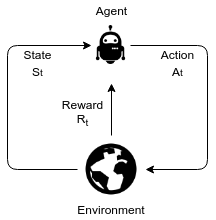
\includegraphics[width=6cm, height=6cm]{./figures/agent_env}
\caption{The interaction between an agent and an environment}
\label{agent_env}
\end{figure}

\subsection{Markov Decision Process (MDP)}
\label{mdp_subsection}
An agent interacts with an environment in a sequence of discrete time steps, which is part of the sequential history of observations, actions and rewards. The sequential history is formalised as 
\begin{equation}
\begin{split}
H\textsubscript{t} = S\textsubscript{1}, R\textsubscript{1}, A\textsubscript{1}, ..., A\textsubscript{t-1}, S\textsubscript{t}, R\textsubscript{t}.  
\end{split}
\end{equation}
where S is \textit{states}, R is \textit{rewards} and A is \textit{actions}. A state S\textsubscript{t} determines the next environment and has a \textit{Markov property} if and only if 
\begin{equation}
\begin{split}
\mathbb{P}[S\textsubscript{t+1} \vert S\textsubscript{t}] = \mathbb{P}[S\textsubscript{t+1} \vert S\textsubscript{1}, ..., S\textsubscript{t}].
\end{split}
\end{equation}
In other words, the probability of reaching S\textsubscript{t+1} depends only on S\textsubscript{t}, which captures all the relevant information from the earlier history (\cite{puterman2014markov}).
When an agent must make a sequence of decision, the sequential decision problem can be formalised using the \textit{Markov decision process (MDP)}. MDP formally represents a fully observable environment of an agent for 
RL.
\begin{defn}{Markov Decision Process (MDP)}

\textit{Markov decision process (MDP)} is defined in the form of a tuple $\langle$S, A, T, R$\rangle$ where:
\begin{itemize}
\item S is the set of finite states that is observable in the environment.
\item A is the set of finite actions taken by the agent.
\item T is \textit{a state transition function}: S $\times$ A $\times$ S $\rightarrow$ [0,1], which is a probability of reaching a future state s$^\prime$ $\in$ S by taking an action a $\in$ A in the current state  s $\in$ S.
%\item T\textsubscript{a}(s, s$^\prime$) is a state transition in the form of probability matrix Pr(S\textsubscript{t+1} = s$^\prime$ $\vert$ s\textsubscript{t} = s, a\textsubscript{t} = a), which is the probability that action \textit{a} in state \textit{s} at time \textit{t} will result in state \textit{s$^\prime$} at time \textit{t+1}.
\item R is a reward function R\textsubscript{a}(s, s$^\prime$) = $\mathbb{P}[R\textsubscript{t+1} $ $\vert$ S\textsubscript{t+1} = s$^\prime$, A\textsubscript{t} = a, S\textsubscript{t} = s], the expected immediate reward that action \textit{a} in state \textit{s} at time \textit{t} will return.
\end{itemize}
\end{defn}

The objective of an agent is to solve an MDP by taking a sequence of actions to maximise the total cumulative reward it receives. 
A method of finding the optimal solution of an MDP is Reinforcement Learning (RL). 
Formally, the objective of a RL agent is to maximise \textit{expected discounted return} over time steps \textit{k},which is defined as:
\begin{equation}
\begin{split}
G\textsubscript{t} = R\textsubscript{t+1} + \gamma R \textsubscript{t+2} + ...  = \sum_{k=0}^{\infty} \gamma\textsuperscript{k} R\textsubscript{t+k+1} 
\end{split}
\end{equation}

where $\gamma$ is a discount rate $\gamma$ $\in$ [0,1], a parameter which represents the preference of the agent for the present reward over future rewards. If $\gamma$ is low, the agent is more interested in maximising immediate rewards. 

\subsection{Policies and Value Functions}
\label{policy_value_functions_subsection}
Most RL algorithms are concerned with estimating \textit{Value functions}.
Value functions estimate the expected return, or discounted cumulative future reward,  for a given action in a given state. The expected reward for an agent is dependent on the agent's action.  
The state value function v\textsubscript{$\pi$}(s) of an MDP under a policy $\pi$ is the expected return starting from state \textit{s}, which is of the form:

\begin{equation}
v\textsubscript{$\pi$}(s) = \displaystyle \E [G\textsubscript{t} \vert S\textsubscript{t} = s] \ \textsf{for all}\ s \in \mathcal{S}
\end{equation}

The optimal state-value function v\textsuperscript{*}(s) maximises the value function over all policies in the MDP, which is of the form:

\begin{equation}
v\textsuperscript{*}(s) = \underset{\pi}{\max} \ v\textsubscript{$\pi$}(s)
\end{equation}

% \begin{examp} \normalfont (Value Functions).

% XXX
% \end{examp}
Value functions are defined by \textit{policies}, which map from states to probabilities of choosing each action. 
A policy $\pi$ is defined as follows:
\begin{equation}
\label{eq:policy}
\begin{split}
\pi(a|s) =  \displaystyle \mathbb{P}[A\textsubscript{t} = a | S\textsubscript{t} = s]
\end{split}
\end{equation}

While the value functions estimate the value of  a particular state, the value of taking an action a given a particular s state is similarly estimated by an \textit{state-action value function}, or \textit{Q function} under a policy $\pi$. State-action value function is defined as follows: 
\begin{equation}
q\textsubscript{$\pi$}(s, a) = \displaystyle \E [G\textsubscript{t} \vert S\textsubscript{t} = s, A\textsubscript{t} = a] \ \textsf{for all}\ s \in \mathcal{S}
\end{equation}

An optimal policy achieves the optimal state-action value functions, and it can be computed by maximising over the optimal state-action value functions.
The optimal state-action-value function q\textsuperscript{*}(s,a) maximises the state-action value functions over all policies in the MDP, which is of the form:

\begin{equation}
q\textsuperscript{*}(s, a) = \underset{\pi}{\max} \ q\textsubscript{$\pi$}(s, a)
\end{equation}

% \begin{examp} \normalfont (State-action value Functions).

% XXX
% \end{examp}

%Among all possible value functions, an \textit{optimal policy $\pi^*$} is the one that maximise the total rewards in the environment.
%The optimal policy $\pi$\textsuperscript{*} corresponds to v\textsuperscript{*}(s)

%\begin{equation}
%\pi \textsuperscript{*} =
%%\pi \textsuperscript{*} = arg max v\textsubscript{\pi}(s)
%\end{equation}

%Reinforcement learning is a method to get approximated optimal solution.
%TODO on-policy and off-policy learning.

%A\textsubscript{t} = $\pi$(S\textsubscript{t})
%
%One of the common possibilities is that the agent chooses an action in order to maximise the discounted sum of future rewards.
%
%A\textsubscript{t} to maximise R\textsubscript{t+1} + $\gamma$ R\textsubscript{t+2} + $\gamma^2$ R\textsubscript{t+3} + ...
%
%An action-value function evaluate a particular state by taking an action according the policy
%
%q\textsubscript{$\pi$} = $\displaystyle \E[R\textsubscript{t+1} $[R\textsubscript{t+1} + $\gamma$ R\textsubscript{t+2} + $\gamma^2$ R\textsubscript{t+3} + ... $\vert$ S\textsubscript{t} = s, A\textsubscript{t} = a, A\textsubscript{t+1 } = a,]

\subsection{Temporal-Difference (TD) Learning}
\label{td_learning_section}

One of the RL approaches for solving a MDP is called \textit{Temporal-Difference (TD) Learning}.
TD learning is an online model-free RL which learns directly from episodes of incomplete experiences without a model of the environment.
TD learning updates the estimates of value function as follows:

\begin{equation}
\centering
V(S\textsubscript{t}) \leftarrow V(S\textsubscript{t}) + \alpha[R\textsubscript{t+1} + \gamma V(S\textsubscript{t+1}) - V(S\textsubscript{t})]
\end{equation}

where R\textsubscript{t+1} + $\gamma$ V(S\textsubscript{t+1}) is the target for TD update, which is a biased estimate of v\textsubscript{$\pi$} (S\textsubscript{t}), and $\delta$ = R\textsubscript{t+1} + $\gamma$ V(S\textsubscript{t+1}) - V(S\textsubscript{t}) is called \textit{TD error}, which is the error in V(S\textsubscript{t}) available at time t+1.
Since the TD learning only needs to know the estimate of one step ahead and does not need the final outcome of the episodes (also called TD(0)), it can learn online after every time step. TD learning also works without the terminal state, which is the goal for an agent.
TD(0) is proved to converge to v\textsubscript{$\pi$} in the table-based case.

%\begin{equation}
%\textbf{	V(S\textsubscript{t} \leftarrow V(S\textsubscript{t} + \alpha (R\textsubscript{t+1} + \gamma V(S\textsubscript{t+1}) - V(S\textsubscript{t}))
%}\end{equation}

\textit{Q-learning} is off-policy TD learning introduced in \cite{Watkins}, where the agent only knows about the possible states and actions.  
The transition states and reward probability functions are unknown to the agent.
The update rule for the state-action value function, called \textit{Q function}, is of the form:

\begin{equation}\label{eq:q_learning}
Q(s\textsubscript{t},a\textsubscript{t}) \leftarrow Q(s\textsubscript{t},a\textsubscript{t}) +  \alpha(R\textsubscript{t+1} + \gamma \ max (a+t) \ Q(s\textsubscript{t+1}, a\textsubscript{t+1}) - Q(s\textsubscript{t}, a\textsubscript{t}))
\end{equation}

where $\alpha$ is a constant step-size parameter, or learning rate, $\alpha$ between 0 and 1,  and $\gamma$ is a discount rate. 
The function Q(S,A) predicts the best action A in state S to maximise the total cumulative rewards. Q-learning is off-policy because a policy being evaluated and improved is different from the policy being used to take an action.

\begin{algorithm}
\caption{Q-learning for leaning $Q$}
\label{algorithm:q_learning}
\begin{algorithmic}[1]
\Procedure{}{}
\State $\text{Initialise $Q(s,a)$ arbitrarily}$
\Repeat$\text{\ for each episode}$
\State $\text{Choose $a$ from $s$ using policy derived from Q}$
\State $\text{Take action $a$, observe $r$,  $s^\prime$}$
\State $Q(s\textsubscript{t},a\textsubscript{t}) \leftarrow Q(s\textsubscript{t},a\textsubscript{t}) +  \alpha(R\textsubscript{t+1} + \gamma \ max (a+t) \ Q(s\textsubscript{t+1}, a\textsubscript{t+1}) - Q(s\textsubscript{t}, a\textsubscript{t}))$
\State $ s \leftarrow s^\prime $
\Until $\text{ $s$ is terminal}$ 
\Return $Q$ 
\EndProcedure

\end{algorithmic}
\end{algorithm}

\begin{equation}
Q(s\textsubscript{t},a\textsubscript{t}) = \displaystyle \E [R\textsubscript{t+1} + \gamma R\textsubscript{t+2} + \gamma^2 R\textsubscript{t+3} + ... \vert s\textsubscript{t},a\textsubscript{t} ]
\end{equation}

Q-learning algorithm is defined in Algorithm \ref{algorithm:q_learning}. Since the state-action value function Q learnt by Q-learning directly approximates q*, Q-learning is  guaranteed to converge to an optimal policy in a finite tabular representation. \textcolor{red}{TODO REF}
Since Q-learning is one of the most widely used RL methods and our experiments are conducted in a tabular representation, we use it as one of the benchmarks for our new framework.
%\textcolor{red}{Paper Jaakkola et al. 1993}

%The optimal Q-function Q\textsuperscript{*}(s,a) is directly approximated by the learned action-value function Q.

% Model free can be done using Monte Carlo Policy evaluation
% One way to solve the Bellman Optimality equation is Q-learning
% U(s) = max a Q(s,a)
% The function is estimated by Q-learning, which repeatedly updates Q(s,a) using the Bellman Equation.
%Q-learning learns the value of its deterministic greedy policy from the experience and gradually converge to the optimal Q-function. It also explored following \textit{$\epsilon$-greedy policy}, which is a stochastic greedy policy, but with the probability of $\epsilon$, the agent chooses an action randomly instead of the greedy action.


\subsection{Model-based and Model-free RL}
\label{model_base_model_free_subsection}
A \textit{model} is a representation of an environment that an agent can use to understand how the environment should look like, which is  T and R in MDP. 
There are two different types of RL methods: \textit{model-based} and \textit{model-free} RL method. 
Model-based RL is where, when a model of the environment is known, the agent uses the model to plan for a series of actions to achieve the agent's goal. 
The model itself can be learnt by interacting with the environment by taking actions, which return states and rewards, and the parameters of the action models can be estimated with maximum likelihood methods \cite{Ray2010}.
Using a model, an agent can do planning to generate or improve a policy for the modelled environment. 

By contrast, model-free RL is where a model is unknown and the agent learns to achieve the goal solely by interacting with the environment without using the model. 
Thus the agent knows only possible states and actions, and the transition state and reward probability functions are unknown.
When the model of the environment is correct, the model-based RL agent can reach an optimal policy without trial-and-error interactions with the environment. 
When the model is not a true representation of the environment, or the true MDP, however, the planning algorithms will not lead to the optimal policy, but a sub-optimal policy.

One algorithm which combines both aspects of model-based and model-free learning to solve the issue of sub-optimality is called Dyna \cite{Sutton1990}.
Dyna learns a model from real experience and uses the model to generate simulated experience to update the evaluation functions.
This approach is more efficient because the simulated experiences are relatively easy to generate compared to real experiences, thus less iterations are required.

This idea of learning a model of the environment and using it to execute planning is a core idea of our new framework. 

\subsection{Transfer Learning}
\label{transfer_learning}

Transfer learning is a method that knowledge learnt in one or more tasks can be used to learn a new task better than if without the knowledge in the first task. Since training a RL algorithm tends to be time consuming and computational expensive, transfer learning allows the trained agent to be applied in a different setting.
While transfer learning is an active research areas in machine learning, not many have been done in RL. Transfer learning in RL is particularly important since most of the RL research have been done in a simulation or game scenarios, and training RL models in a real physical environment is more expensive to conduct. Even in a virtual environments like games, the transfer learning between different tasks will greatly will have a big impact on potential applications.
One of the purposes of transfer learning is so that the agent requires less time to learn a new task with the help of what was learn in previous tasks. Another goal would be to measure how effectively the agent reuses its knowledge in a new task.
% There are many different matrices used to measure the performance of the transfer learning.
% Five common metrics are defined in XX as follow.
% TODO source task selection
%Compare with human play, which is used in DeepMind Atari paper.
% Since each metric measures different aspect of transfer learning, using multiple metrics would provide more comprehensive views of the performance of an RL algorithm.

% \subsection{Function Approximation}
% \label{function_approximation}
% Q-learning with a tabular representation works when every state-action value can be represented. 
% In case of very large MDPs, however, it may not be possible to represent all state-action values with a tabular representation.
% For example, robot arms have a continuous states in 3D dimensional space.
% This problem motivates the use of \textit{function approximation}, which estimates value function with function approximation.  Not only is it represented in tabular form, but also in the form of a parameterised function with \textit{weight vector w}.
% %$\in \R\textsuperscript{d}$ where $\R\textsuperscript{d}$ is XXX
% Unlike Q-table, changing one weight updates the estimated value of not only one state, but many states, and this generalisation makes it more flexible to apply to different scenarios where the tabular approach could not be applied.

% The reason we are introducing the function approximation is that it is used as another benchmark for our new framework.

% \subsubsection{The Prediction Objective ($\overline{VE}$)}
% With function approximation, an update at one state changes many other states, and therefore the values of all states will not be exactly accurate.
% There is a trade off among states as to which state we make it more accurate, while others might be less accurate.
% The error in a state s is the square of the difference between the approximate value $\hat{v}$(s,w) and the true value v\textsubscript{$\pi$}(s). The objective function can be defined by weighting it over the state space by $\mu$, the \textit{Mean Squared Value Error}, denoted $\overline{VE}$.

% \begin{equation}
% \overline{VE}(w) \doteq \sum_{s \in S} \mu (s) \big[ v\textsubscript{$\pi$}(s) - \hat{v}(s,w) \big]\textsuperscript{2}.
% \end{equation}
% \label{ve}

% \subsubsection{Stochastic gradient descent (SGD)}
% \textit{Stochastic gradient descent (SGD)} methods are commonly used to learn function approximation in value prediction, which works well for online reinforcement learning.
% %TODO EXPLAIN ONLINE VS OFFLINE LEARNING
% The weight vector w in SGD is defined as:
% \begin{equation}
%  w \doteq  \begin{pmatrix}  w\textsubscript{1}  \\ w\textsubscript{2} \\ \vdots \\ w\textsubscript{n}   \end{pmatrix}
% \end{equation}

% and $\hat{v}$(s,w) is a differentiable function of w for all s $\in$ S.
% %minimize the $\overline{VE}$ on the observed examples. 
% SGD adjusts the weights vector by a fraction of $\alpha$, a step-size parameter,  in the direction that reduces the error on that example the most. Formally, it is defined as:

% \begin{equation}\label{eq:sgd}
% \begin{split}
% w\textsubscript{t+1} & \doteq w\textsubscript{t} -  \frac{1}{2} \alpha  \bigtriangledown \big[ v\textsubscript{$\pi$}(S\textsubscript{t}) - \hat{v}(S\textsubscript{t}, w\textsubscript{t}) \big]\textsuperscript{2}. \\
% & = w\textsubscript{t} +  \alpha  \big[ v\textsubscript{$\pi$}(S\textsubscript{t}) - \hat{v}(S\textsubscript{t}, w\textsubscript{t}) \big] \bigtriangledown \hat{v}(S\textsubscript{t}, w\textsubscript{t}).
% \end{split}
% \end{equation}

% The gradient of J(w), which is the vector of partial derivatives with respect to each weight vector,  is defined as:

% \begin{equation}
% \bigtriangledown\textsubscript{w} J(w) =  \begin{pmatrix} \frac{\partial J(w)}{\partial w\textsubscript{1}}  \\ \vdots \\ \frac{\partial J(w)}{\partial w\textsubscript{n}}   \end{pmatrix}
% \end{equation}

% %\begin{equation}
% %w\textsubscript{t+1} \doteq w\textsubscript{t} + \alpha \big[ U\textsubscript{t} - \hat{v}(S\textsubscript{t}, w\textsubscript{t})\big] x(S\textsubscript{t})
% %\end{equation}

% \subsubsection{Linear Value Function Approximation}
% A \textit{linear function} of a weight vector is a type of simple function approximation to approximate the action-value function. 
% \begin{equation}
% \hat{q}(s,a) \approx q\textsubscript{$\pi$} (s,a)
% \end{equation}

% The vector x(s,a) represents a \textit{feature vector}, which is of the form:

% \begin{equation}
% x(S, A) = \begin{pmatrix} x\textsubscript{1}(S, A) \\ \vdots \\ x\textsubscript{n}(S, A)  \end{pmatrix}
% \end{equation}
% where each x(s,a) is a feature of the corresponding action-state pair.

% Using the SGD update with linear function approximation, the gradient of the approximate value function with respect to w is:
% %\textcolor{red}{Add proof here}
% \begin{equation}
% \bigtriangledown \hat{q}(s, a,w) = x(s, a)
% \end{equation}

% Thus the general SGD update defined in (\ref{eq:sgd}) can be simplified to the following:

% \begin{equation}\label{eq:sgd_linear}
% \begin{split}
% w\textsubscript{t+1} & = w\textsubscript{t} +  \alpha  \big[ q\textsubscript{$\pi$}(S\textsubscript{t}, A\textsubscript{t}) - \hat{q}(S\textsubscript{t}, A\textsubscript{t}, w\textsubscript{t}) \big] x(S\textsubscript{t}, A\textsubscript{t})
% \end{split}
% \end{equation}

% %The error in a state s is the square of the difference between the approximate value
% %$\hat{v}$(S,w) and the true value v(S,w).
% %\begin{equation}
% %J(w) = \displaystyle \E \textsubscript{$\pi$} \big[ (v\textsubscript{$\pi$}(S) -  \hat{v}(S,w))\textsuperscript{2} \big]
% %\end{equation}
% Unlike non-linear value function approximation, the linear method is guaranteed to converge to a global optimum.
% One disadvantage of the linear method is that it cannot express any relationship between features. For example, it cannot represent that feature \textit{i} is useful only if feature \textit{j} is not present.
% Nevertheless,  this approach is sufficient for our experiments, which are described in Chapter \ref{evaluation}.

% \subsubsection{Tile Coding \textcolor{red}{(TBD)}}
% There are different linear function approximation methods to represents states as features. Feature construction depends on a problem you are solving.  We introduce \textit{Tile Coding} which will be used for our benchmark.
% \begin{figure}[!htb]
% \centering
% 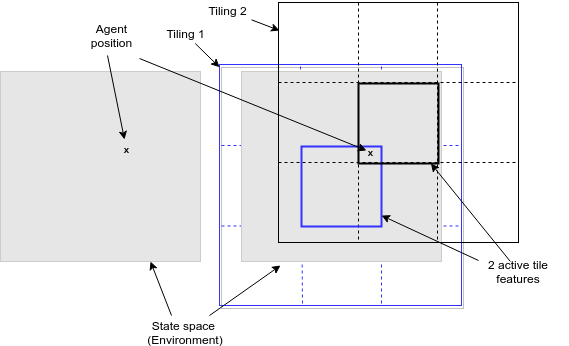
\includegraphics[width=1.0\textwidth]{./figures/tile_coding}
% \caption{Tiling coding illustration}
% \label{fig:tile_coding}
% \end{figure}

% Illustration of tile coding is shown in Figure \ref{fig:tile_coding}. In Tile Coding, state set is represented as a continuous two-dimentionala space. If a state is within the space, then the value of the  corresponding feature is set to be 1 to indicate that the feature is present, while 0 indicates that the feature is absent. This way of representing the feature is called \textit{binary feature}.  \textit{Coarse coding} represents a state with which binary features are present within the space.
% One area is associated with one weight w, and training at a state will affect the weight of all the areas overlapping that state. the approximate value function will be updated within at all states within the union of the areas, and a point that has more overlap will be more affected.
% The size and shape of the areas will determine the degree of the generalisation. Large areas will have more generalisation. In addition, tiles can be overlap, and the change of the weight in that state will affect all other states within the intersection of the spaces. 
% The degree of overlap within a space will determined the degree of the generalisation.
% The shape of the space also affect how it is generalised.

% \textit{Tile coding} is a type of coarse coding. \textit{Tiling} is a partition of state space, and each element of the partition is called a \textit{tile}.

% The state space is partitioned into multiple tiles with multiple tilings. Each tile in each tiling is associated with

% In order to do coarse coding with tile coding, multiple tilings are required, each tiling is offset from one another by a fraction of a tile width.

% As illustrated in Figure XXX, when a state occurs, several features with corresponding tiles become active,

% Tile coding has computational advantage, since each component of tiling is binary value, .

% a trained state will be generalised to other states if they are within any of the same tiles.

% Similar to coarse coding, the size and shape of tiles will determine the degree of approximation.

\chapter{Framework}
\label{framework}
This chapter introduces a new proof-of-concept framework called \textit{ILP(RL)}, a new learning framework for solving MDP problems using inductive learning with ILASP and planning with ASP.
The development of this framework is one of the main objectives of this project and we explain the framework in details in this Chapter.

\section{Overview}
\label{sec:overview}

\begin{figure}[!htb]
\centering
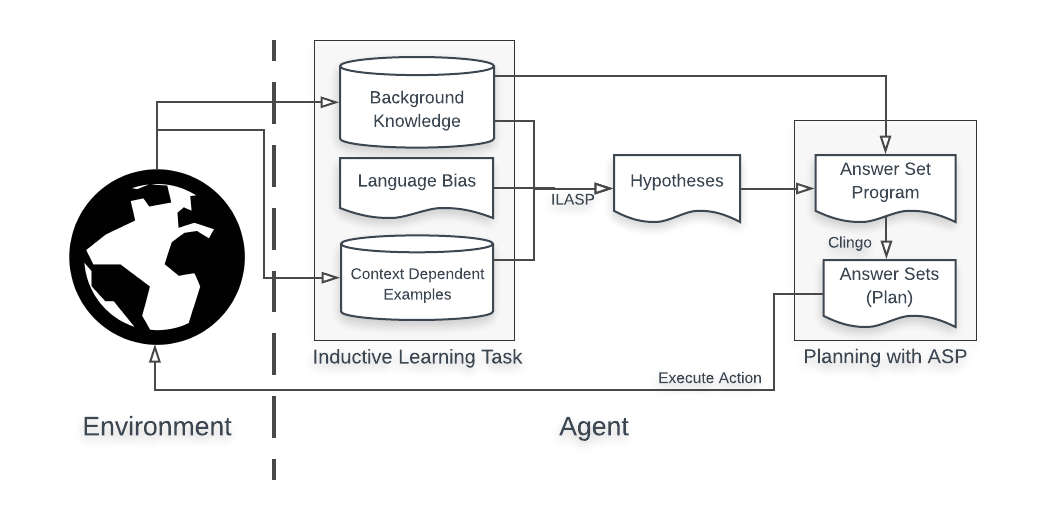
\includegraphics[width=1.0\textwidth]{./figures/architecture}
\caption{ILP(RL) overview}
\label{fig:ILPRL_overview}
\end{figure}


\begin{algorithm}
\caption{Inductive Learning ILP(RL) Algorithm}
\label{algorithm:inductive_learning}
\begin{algorithmic}[1]
\label{algo:ILPRL}
\renewcommand{\algorithmicrequire}{\textbf{Input:}}
\State \textbf{Input:}
\State \ \ \ \ \ \ Current hypothesis $H$
\State \ \ \ \ \ \ Cumulative context dependent examples $E$
\State \ \ \ \ \ \ Background knowledge$B$
\State \ \ \ \ \ \ Language bias $S\textsubscript{M}$ \\
\Procedure{Inductive-Learning}{$H, E, B, S\textsubscript{M}$}
\If {$ILASP(B \cup H \cup S\textsubscript{M}=\emptyset)$ does not cover $E$}
\State $H = ILASP(B, S\textsubscript{M}, E)$
\EndIf
\State $Update(B, e)$
\LineComment{Add surrounding walls to $B$}

\EndProcedure
\end{algorithmic}
\end{algorithm}


% \begin{algorithm}
% \caption{ILP(RL) Algorithm}
% \begin{algorithmic}[1]
% \label{algo:ILPRL}
% \renewcommand{\algorithmicrequire}{\textbf{Input:}}
% \State \textbf{Input:}
% \State \ \ \ \ \ \ States $S = \{ 1, ..., n\textsubscript{x}\}$
% \State \ \ \ \ \ \ Actions $A = \{ 1, ..., n\textsubscript{a}\} A: X \rightarrow A$
% \State \ \ \ \ \ \ States transition $T: X \times A \rightarrow X$
% \State \ \ \ \ \ \ $\epsilon \in [0,1]$
% \State \ \ \ \ \ \ Background knowledge for ILASP and ASP $B$
% \State \ \ \ \ \ \ Language bias $S\textsubscript{M}$ \\

% \Procedure{ILP(RL)}{$S, A, T, \epsilon, B, S\textsubscript{M}$}
% \State {$H = \emptyset$}
% \State {$E = \emptyset$}
% \State {Start s $\in$ S}
% \While {$s$ is not terminal} 
% \State $a \leftarrow POLICY(s, A, B, H, \epsilon)$ \\
% \space
% \LineComment{observe the next state $s^\prime$ by taking action a}
% \State $s^\prime \leftarrow T(s,a)$
% \space
% \LineComment{generate a positive example}
% \State $e \leftarrow MakeDCPI(s^\prime, s, a) $ 
% \State $E = E + e$
% \space
% \LineComment{if the current B $\cup$ H without language bias does not cover E, update H}
% \If {$ ILASP(B \cup H, S\textsubscript{M}=\emptyset, E) == UNSATISFIABLE$}
% \State $H = ILASP(B, S\textsubscript{M}, E)$
% \EndIf
% \State $Update(B)$
% \EndWhile
% \EndProcedure
% \end{algorithmic}
% \end{algorithm}

The overall architecture of ILP(RL), is shown in Figure \ref{fig:ILPRL_overview}. 
ILP(RL) mainly consists of two components: inductive learning with ILASP and planning with ASP. 

The first step is inductive learning. An agent interacts with an unknown environment, 
and receives state transition experiences as context dependent examples. 
Together with pre-defined background knowledge and language bias, these examples are used to inductively learn and improve hypotheses, which are state transition function in the environment.

The second step is ASP planning. The interaction with the environment also gives the agent information about the environment, such as locations of walls or a terminal state. 
The agent remembers these information as background knowledge, and, 
together with the learnt hypotheses, uses them to make an action plan by solving an ASP program.
The plan is a sequence of actions and it navigates the agent in the environment.

The agent iteratively executes this cycle in order to learn and improve the hypotheses as well as an action planning. 
Mechanisms of each step are explained in details in the following sections.

\section{Environment}
\label{sec:environment}
Since there is no existing base frameworks for ILP(RL), our focus on this project is to develop a preliminary version of the framework. 
Therefore, we use a very simple environment that allows us to see the potentials of our proposed architecture.
The base environment is a simple grid maze, and we assume that the environment is a discrete deterministic environment. 

We use a simple example to explain the environment as shown in Figure \ref{environment_example}.
States are expressed as X and Y coordinates. In Figure \ref{environment_example}, for example, the agent is located at \{X=2, Y=4\}.
The agent can take one of four possible actions at each time: up, down right and left.
Every time the agent takes an action, the agent receives the following experiences: a reward R\textsubscript{t}, the next state S\textsubscript{t+1} and surrounding information of the current state.
The base environment mainly consists of three different elements: a goal, walls and paths.
The goal cell is the terminal state and the agent receives a positive reward when the agent receives a negative reward in any states except the terminal state.
When the agent reaches the terminal state, the agent receives a positive reward and the current episode is complete. 
Since the agent's goal is to maximise the total estimate rewards over time, this goal is equivalent to finding the shortest path from a starting state to a terminal state.

We also assume that, unlike an agent with other RL algorithms, the agent can see states of vertical and horizontal, but not diagonal, states around the agent. 
This assumption allows a agent to learn a state transition in the environment using inductive learning. For example, the agent at \{X=2, Y=4\} can see that there are walls at \{X=1, Y=4\} and \{X=2, Y=5\}.
More details of how to use these surrounding information is described in \ref{sec:inductive_learning_task}.

The applicability for a more complex environment is not considered in this project and it is discussed in Further Research in Section \ref{sec:further_research}.

% The environment is provided outside of our algorithm,
\begin{figure}[!htb]
\centering
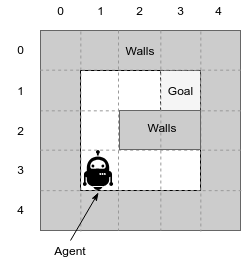
\includegraphics[width=0.4\textwidth]{./figures/environment_example}
\caption{5$\times$5 grid maze example}
\label{environment_example}
\end{figure}

\section{Inductive Learning Task}
\label{sec:inductive_learning_task}
The first step is to construct a learning task using ILASP. The objective of the inductive learning is to learn state transitions in a given environment, which is used for generating an action plan at later steps.
The target hypotheses are specified as follows:

\begin{equation}
\begin{split}
&\textsf{state\_after(V1):-adjacent(right, V0, V1), state\_before(V1), action(right), wall(V0).}\\
&\textsf{state\_after(V0):-adjacent(right, V0, V1), state\_before(V1), action(right), not wall(V0).}\\
&\textsf{state\_after(V1):-adjacent(left, V0, V1), state\_before(V1), action(left), wall(V0).}\\
&\textsf{state\_after(V0):-adjacent(left, V0, V1), state\_before(V1), action(left), not wall(V0).}\\
&\textsf{state\_after(V1):-adjacent(down, V0, V1), state\_before(V1), action(down), wall(V0).}\\
&\textsf{state\_after(V0):-adjacent(down, V0, V1), state\_before(V1), action(down), not wall(V0).}\\
&\textsf{state\_after(V1):-adjacent(up, V0, V1), state\_before(V1),  action(up), wall(V0).}\\
&\textsf{state\_after(V0):-adjacent(up, V0, V1), state\_before(V1), action(up), not wall(V0).}
\end{split}
\label{target_hypothesis}
\end{equation}

where \textsf{state\_after} is the next state S\textsubscript{t+1}, \textsf{state\_before} is the current state S\textsubscript{t}. \textsf{action} is an action A\textsubscript{t} taken by the agent.
\textsf{adjacent(D, V0, V1)} specifies that V0 is next to V1 in the direction of D. For example, \textsf{adjacent(right, V0, V1)} means V0 is right next to V1. 
\textsf{wall(V)} and \textsf{not wall(V)} specify whether a state is a wall or not wall in a state V respectively.
We describe the details of how to construct the background knowledge, context dependent examples and the language bias in the following sections, and these are the necessary components for the agent to learn the target hypotheses.
% The summary of a full ILASP learning task can be found in Appendix \ref{chap:learning_tasks}.
% Similar to other RL algorithms, an agent explores an environment by taking actions, which generates experiences. 
% These experiences need to be translated into ASP syntax and 
% and are recorded in as context dependent examples. 
% a positive example and background knowledge.
% Positive examples and background knowledge are used by ILASP for inductive learning, and background knowledge is used by both ILASP and ASP for solving for answer sets.

\subsection{Background Knowledge}
\label{subsec:background_knowledge}
First we define necessary background knowledge for the inductive learning.
In order to learn the state transition for each direction as shown in \ref{target_hypothesis}, we need to define the meaning of "being next to" a state.
This is defined as a rule \textit{adjacent}, which is of the form:

\begin{equation} \label{eq:adjacent}
\begin{split}
&\textsf{adjacent(right, (X+1,Y),(X,Y)):-cell((X,Y)), cell((X+1,Y)).} \\
&\textsf{adjacent(left,(X,Y),  (X+1,Y)):-cell((X,Y)), cell((X+1,Y)).} \\
&\textsf{adjacent(down, (X,Y+1),(X,Y)):-cell((X,Y)), cell((X,Y+1)).} \\
&\textsf{adjacent(up,   (X,Y),  (X,Y+1)):-cell((X,Y)), cell((X,Y+1)).} \\
\end{split}
\end{equation}

where \textsf{cell} corresponds to a state, and \textsf{X} and \textsf{Y} represent x-coordinate and y-coordinate respectively.
The rules \ref{eq:adjacent} are given as background knowledge and allow the agent to understand the relation of two adjacent states.
\textit{cell((X,Y))} is defined as follows:
\begin{equation} \label{eq:cell}
\begin{split}
    &\textsf{cell((0..X, 0..Y)).}
\end{split}
\end{equation}

where, \textsf{X} and \textsf{Y} are the size of width and height of an environment respectively. 
For example, a grid maze shown in Figure\ref{environment_example} has a height and width of 4, thus the type cell is defined in the background knowledge as \textsf{cell((0..4, 0..4))}.

\subsection{Context Dependent Examples}
\label{subsec:context_dependent_examples}
Context dependent examples contain actual state transition that the agent gains by interacting with an environment. Since all the interactions with the environment are examples of valid moves,
they are used as positive examples. A positive example is expressed as a following ASP form:
\begin{equation}
\begin{split}
    \textsf{\#pos}(\{E\SPSB{inc}{ILP(RL)}\}, \{E\SPSB{exc}{ILP(RL)}\}, \{C\textsubscript{ILP(RL)}\})
\end{split}
\end{equation}

It is equivalent to context-dependent partial interpretation (CDPI) in  $ILP_{LAS}^{context}$. 
As defined in the Equation \ref{eq:cdpi}, CDPI is of the form $\langle e, C \rangle$ where $e = \langle E\textsuperscript{inc}, E\textsuperscript{exc} \rangle$. 
Each of the component in CDPI in ILP(RL) is defined as follows:

\begin{defn}\label{def:ILPRL_context}
$C\textsubscript{ILP(RL)}$ contains an action a\textsubscript{t}, the current state $s\textsubscript{t}$, and adjacent walls of $s\textsubscript{t}$.
\label{def:context}
\end{defn}

\begin{defn} \label{def:ILPRL_inc}
$E\SPSB{inc}{ILP(RL)}$ includes $s\textsubscript{t+1} \in S$ such that:
\begin{itemize}
\item s\textsubscript{t+1} = s\textsuperscript{*}\textsubscript{t+1}
\item $ \forall A \in AS(B \cup H\textsubscript{t} \cup C\textsubscript{ILP(RL)})|$ s\textsubscript{t+1} $\not\in A$
\end{itemize}
\end{defn}

\begin{defn} \label{def:ILPRL_exc}
$E\SPSB{exc}{ILP(RL)}$ includes $s\textsubscript{t+1} \in S$ such that:
\begin{itemize}
\item $s\textsubscript{t+1} \neq s\textsuperscript{*}\textsubscript{t+1}$
\item $ \exists A \in AS(B \cup H\textsubscript{t} \cup C\textsubscript{ILP(RL)})|$ s\textsubscript{t+1} $\in A$
\end{itemize}
\end{defn}

where $s\textsuperscript{*}\textsubscript{t+1}$ is the true next state where the agent is at $t+1$, 
$B$ is the background knowledge, $H\textsubscript{t}$ is the hypotheses at $t$, $S$ is all the states in the environment.

% For context C, a\textsubscript{t} is translated int \textit{action((a))}, s\textsubscript{t} is translated into \textit{state\_before((x,y))}, and adjacent walls of s\textsubscript{t} are translated into \textit{wall((x$^\prime$,y$^\prime$))}.

% In this report, we assume that part of context contains only whether a wall exists or not, with the presence of a wall, the agent cannot move to the state where a wall exists.

% \subsubsection{Positive examples in ASP syntax}
% \label{subsubsec:positive_examples_asp_syntax}

% For example, if the agent takes an action "up" to move from (1,1) to (1,2), all other states that the agent could have taken but did not are exclusions ((1,0), (1,1), (0,1) and (2,1) in this case).
% context examples include state\_before((X1,Y1)), which represents the position of the agent in x and y axis before an action is taken,
% action(A) is the action the agent has taken, and surrounding information, such as surrounding walls.

% Rewards are not used.
% (Discussed in details in Chapter XX).

% \textcolor{red}{There is no negative example as XXXX.}
% Using these positive examples, the agent is able to learn and improve hypothesis as it explore the environment and encounters new scenarios.
\begin{examp} \normalfont (Context dependent examples).

\begin{figure}[!htb]
\centering
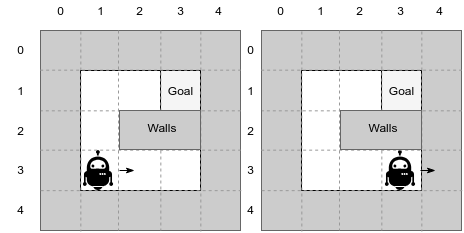
\includegraphics[width=0.8\textwidth]{./figures/env_context_example}
\caption{5$\times$5 grid maze example (context dependent example)}
\label{example_pos_example}
\end{figure}

We use a simple $5 \times 5$ grid maze environment to highlight how an agent gains a positive example.
Suppose $H\textsubscript{t}=\emptyset$ and an agent takes an action "right" to move from $(1,3)$ to $(2,3)$ cell, as shown on the left in Figure \ref{example_pos_example}.
$a\textsubscript{t}$ is "right", $s\textsubscript{t}$ is $(1,3)$ and $s^*\textsubscript{t}$ is $(2,3)$.
According to the Definition \ref{def:ILPRL_inc}, $A=\emptyset$ since $H\textsubscript{t}=\emptyset$, thus \textsf{state\_after((2,3))} is in $E\SPSB{exc}{ILP(RL)}$, $A=\emptyset$ is there is no exclusions in this case.
$C\textsubscript{ILP(RL)}$ includes $a\textsubscript{t}$, $s\textsubscript{t}$ and adjacent walls of $s\textsubscript{t}$.
The following positive example is generated.

\begin{equation}
\begin{split}
    \textsf{\#pos(} & \textsf{\{state\_after((2,3))\},}\\
                    & \textsf{\{\},} \\
    & \textsf{\{state\_before((1,3)). action(right). wall((0, 3)). wall((1, 4)).\})}
\end{split}
\end{equation}

The next example illustrates a case when the agent tries to move to a state where a wall is. As shown on the right in Figure \ref{example_pos_example}, the agent is at $(3,3)$ and tries to move to a state $(3,4)$ by taking an action "right", as shown on the left in Figure \ref{example_pos_example}. 
In this case, however, there is a wall at $(4,3)$ and therefore the agent cannot go to that state. Because of the blocking wall, $s\textsubscript{t} = s^*\textsubscript{t+1} = (4,4)$.
The same the previous case, suppose $H = \emptyset$ and therefore $A = \emptyset$.
% All other alternative next adjacent states S\textsubscript{t+1} (4,3), (3,4), (5,4) and (4,5) are exclusions, and the contexts are collected.
From this example, the following positive example is generated:
\textcolor{red}{TODO UPDATE this example}
\begin{equation}
\begin{split}
\textsf{\#pos(} & \textsf{\{state\_after((4,4))\}}, \\
                & \textsf{\{state\_after((4,3)),state\_after((3,4)),state\_after((5,4)),state\_after((4,5))\}} \\
                & \textsf{\{state\_before((4,4)). action(right). wall((5,4)). wall((4,5)).\}).}
\end{split}
\end{equation}

\end{examp}
\label{state_transition_example}

\subsection{Language Bias}
\label{subsec:language_bias}
We now define a search space using a language bias specified by \textit{mode declaration}.
As defined in \ref{def:las_context}, $H \subseteq S\textsubscript{M}$ for $ILP_{LAS}^{context}$, thus in order to learn the target hypotheses, $S\textsubscript{M}$ is specified as follows:
\begin{equation} \label{eq:sm}
\begin{split}
&\textsf{\#modeh(state\_after(var(cell))).}\\
&\textsf{\#modeb(1, adjacent(const(action), var(cell), var(cell)), (positive)).} \\
&\textsf{\#modeb(1, state\_before(var(cell)), (positive)).} \\
&\textsf{\#modeb(1, action(const(action)),(positive)).} \\
&\textsf{\#modeb(1, wall(var(cell))).} \\
\end{split}
\end{equation}

where \textsf{\#modeh} and \textsf{\#modeb} are the \textit{normal head declarations} and the \textit{body declarations}. 
The first argument of each \textsf{\#modeb} specifies the maximum number of times that \textsf{\#modeb} can be used in each rule (also called \textit{recall}) \cite{Law2017}, 
which we specify $1$ for \textsf{\#modeb} in ILP(RL). \textsf{var(t)} is a placeholder for a variable of \textit{type} \textsf{t}. In \ref{eq:sm}, we use \textsf{cell} for the variable type, which is grounded using \textsf{cell} specified in \ref{eq:cell} in the background knowledge.
\textsf{const(t)} is a placeholder for a constant term of type \textsf{t}, and type \textsf{t} must be specified as \textsf{\#constant(t, c)}, where \textsf{c} is a constant term., 
\textsf{const(t)} is specified as follows:

\begin{equation}
\begin{split}
&\textsf{\#constant(action, right).}\\
&\textsf{\#constant(action, left).}\\
&\textsf{\#constant(action, down).}\\
&\textsf{\#constant(action, up).}
\end{split}
\end{equation}

\textsf{action} type is specified as a constant since ILP(RL) needs to learn a different hypothesis of state transitions for each direction based on the context dependent examples that the agent collects..

\textsf{(positive)} in \textsf{\#modeb} specifies that the body predicates only appear as positive and not negation as failure, which reduces the search space. We use \textsf{(positive)} for all \textsf{\#modeb} except \textsf{wall}. Thus \textsf{wall(var(cell))} could appear as \textsf{not wall} in a hypothesis, and all other body predicates should only be positive.

Finally, we define \textsf{\#max\_penalty} to specify the maximum size of the hypothesis. By default it is 15, however our target hypotheses defined in \ref{target_hypothesis} is larger than 15, and thus it is increased to 50.
Increasing \#max\_penalty allows ILASP to learn longer hypotheses at the expense of longer computation.

\subsection{Hypothesis}
\label{sebsec:hypothesis}
Having defined the $ILP_{LAS}^{context}$ task $T = \langle B, S\textsubscript{M}, E\textsuperscript{+}, E\textsuperscript{-} \rangle$, ILP(RL) is able to learn hypotheses $H$. 
Since $B$ and $S\textsubscript{M}$ are fixed, the hypotheses vary based on context dependent examples that the agent accumulates by interacting with an environment.
For example, in the early phase of learning, the agent does not have many positive examples, and learns a hypothesis that is subset of the full target hypotheses that the agent could learn in the environment. Thus ILP(RL) needs to iteratively improves the hypotheses as illustrated in Figure \ref{fig:ILPRL_overview}.
As specified in line 19 of Algorithm \label{algo:ILPRL}, $ILP_{LAS}^{context}$ is executed when the current hypotheses do not cover the new context example.
If the current hypotheses cover the new positive example, there is no need to re-execute ILASP.
% ILP(RL) runs $ILP_{LAS}^{context}$ to relearn H\textsubscript{new} if and only if $\forall$$\langle$ e, C$\rangle$ $\in$ E\textsuperscript{+}, $\exists$A $\in$ Answer Sets (B $\cup$ C $\cup$ H) such that A extends e
% \end{defn}
% where H is the current hypotheses that the agent has learnt so far. 

The learnt hypotheses will be used for ASP planning, which we describe in the next section.

\begin{examp} \normalfont (Hypothesis).
Using the context dependent examples illustrated in Example \ref{example_pos_example}, we explain how the agent learns hypotheses.
Suppose that the agent takes an action "right" and gains one positive example, as shown on the right in Example \ref{example_pos_example}. 
The full learning task for this simple case is shown as follows:

\lstinputlisting[
  caption  = {Learning task example},
]{learning_task_example1.pl}
From the above learning task, ILASP learns the following hypothesis.
\begin{equation*}
\begin{split}
\textsf{state\_after(V1) :- adjacent(left, V0, V1), state\_before(V0).}
\end{split}
\end{equation*}

After having learnt the hypothesis above, suppose the agent takes another action and gains one extra example as shown in Listing \ref{additional_example}.
\lstinputlisting[
  caption  = {Additional context dependent example},
  label = {additional_example}
]{learning_task_example2.pl}

The current hypothesis, does not cover the new positive example, ILP(RL) runs ILASP with the new positive example. The revised hypotheses are as follows:
\begin{equation*}
\begin{split}
XXX
\end{split}
\end{equation*}

ILP(RL) keeps improving the hypotheses this way until the target hypotheses are learnt.
\end{examp}

\section{Planning with Answer Set Programming}
\label{sec:planning}
The learnt hypotheses in the inductive learning phase are used to generate a sequence of action plan that the agent should follow.
In the following subsections, we explain how to create an ASP program and use the answer sets by the ASP to make an action plan in a maze environment.
\subsection{Answer Set Program}
\label{subsec:answer_set_program}
The ASP program should be constructed such that answer sets of the ASP program are a sequence of actions and states at each time step in ASP syntax. 
The answer set program for ILP(RL) is summarised in Listing \ref{list:asp_planning}:
\lstinputlisting[
  caption  = {Answer set program for ILP(RL)},
  label = {list:asp_planning}
]{asp_planning.pl}
First, we use the learnt hypotheses returned from ILASP as part of the ASP program.
In the inductive learning phase in ILP(RL), we only need to differentiate between $s\textsubscript{t}$ and $s\textsubscript{t+1}$ as \textsf{state\_before} and \textsf{state\_after} respectively.
For the planning with ASP, however, the answer sets contain a sequence of actions and states for more than two time steps, such as $s\textsubscript{t}, s\textsubscript{t+1}, s\textsubscript{t+2}, \dots$.
In order to capture the notion of the time sequences, the ASP syntax of the hypotheses needs to be modified from inductive learning phase to ASP planning by 
adding time \textit{T}. Specifically, the following mapping is required between ILASP and ASP planning syntax.

\begin{table}[H]
\centering
\begin{tabular}{|l|p{5cm}|p{5cm}|}
\hline
No & Inductive learning syntax & ASP planning syntax\\ \hline
1 & \textsf{state\_before(V)} & \textsf{state\_at(V1, T)}  \\ \hline
2 & \textsf{state\_after(V)} & \textsf{state\_at(V1, T+1)}  \\ \hline
3 & \textsf{(empty body)} & \textsf{time(T)}  \\ \hline
4 & \textsf{action(A)} & \textsf{action(A, T)}  \\ \hline
\end{tabular}
\caption{ASP syntax mapping between inductive learning and ASP planning}
\label{table:extension_specification}
\end{table}
The conversion from (empty body) to \textsf{time(T)} means that the body of all the hypotheses includes \textsf{time(T)} in ASP planning syntax.
\begin{examp} \normalfont (Mapping of ASP syntax between inductive learning and ASP planning).

Suppose that an agent learnt the following hypothesis in inductive learning phase. 
\begin{equation*}
\begin{split}
&\textsf{state\_after(V0) :- adjacent(right, V0, V1), state\_before(V1), action(right), not wall(V0).}\\
\end{split}
\end{equation*}

This hypothesis is converted into the following syntax for ASP planning.
\begin{equation*}
\begin{split}
&\textsf{state\_at(V0, T+1) :- time(T), adjacent(right, V0, V1), state\_at(V1, T), action(right, T), not wall(V0).}\\
\end{split}
\end{equation*}
The converted hypothesis is used to generate a sequence of actions and states to the "right" direction for more then two time steps for ASP planning.
\end{examp}

An action for the agent is given as a choice rule, which is of the form:
\begin{equation}\label{eq:choice_rule}
\begin{split}
&\textsf{1\{action(down,T); action(up,T); action(right,T); action(left,T)\}1} \\
&\textsf{ :- time(T), not finished(T).}\\
\end{split}
\end{equation}
The choice rule states that an action must be one of four actions: \textsf{down}, \textsf{up}, \textsf{right}, or \textsf{left}
at each time step T, as defined in the maximum and minimum integers 1.
The choice rule specifies that one of four actions must be true unless \textsf{not finished(T)} or \textsf{time(T)} are satisfied, as defined in the body of the rule.Therefore there is always an action to be taken until the agent reaches a terminal state, 
When the agent reaches a terminal state, \textsf{finished(T)} is satisfied, otherwise time step T exceeds a maximum time step allocated to the agent.

The maximum time step is  specified externally and it is of the form:
\begin{equation}
\begin{split}
&\textsf{time(T\textsubscript{t}..T\textsubscript{max})}
\end{split}
\end{equation}
where T\textsubscript{t} is the current time step and T\textsubscript{max} is the maximum time step.
For example, if an agent is at time step 0, and can take actions up to 100 time step within an episode until it finds a terminal state, \textsf{time} is defined as \textsf{time(0..100)}.

\textsf{finished(T)} determines whether the agent reaches the goal, which is specified as follows:

\begin{equation}\label{eq:asp_goal}
\begin{split}
&\textsf{finished(T):- goal(T2), time(T), T} \geq \textsf{T2.}\\
&\textsf{goal(T):- state\_at((X\textsubscript{terminal}, Y\textsubscript{terminal}), T), not finished(T-1).}\\
&\textsf{goalMet:- goal(T).}\\
&\textsf{:- not goalMet.}
\end{split}
\end{equation}

\textsf{state\_at((X\textsubscript{terminal}, Y\textsubscript{terminal}))} is the location of the terminal state, which is unknown to the agent before the learning starts.
The agent explores the environment until it finds the terminal state. The terminal state is stored in the background knowledge.

Once the agent reaches the goal at time $t$ and \textsf{finished(T)} is satisfied, 
there will not be any actions at time $t+1$ since the body of the choice rule defined in \ref{eq:choice_rule} is not satisfied.

The locations of walls are what the agent collects from the context of context dependent examples, which are specified as follows:
\begin{equation}
\begin{split}
&\textsf{wall((X,Y))}\\
\end{split}
\end{equation}
 
These wall information are accumulated as background knowledge, and they are used for ASP planning. 

The starting state for the planning is provided as part of ASP. It is the current location of the agent at time t when the plan is generated. It is specified as follows:
\begin{equation}
\begin{split}
\textsf{state\_at((X\textsubscript{start}, Y\textsubscript{start}), T)}
\end{split}
\end{equation}

In addition, the definition of adjacent and cell type are also provided, which is the same as the definition of adjacent in inductive learning phase defined in Equation \ref{eq:adjacent} and \ref{eq:cell}.

Next, we need to incorporate a notion of rewards. Instead of maximising the total rewards, which is the objectives of most RL methods, we assume that the rewards for any states except the terminal state in an environment are -1, so that we can use
an optimisation statement in ASP in order to maximise the total rewards. Due to this assumption, the current framework of ILP(RL) works only subset of MDP, and our preliminary research focuses on solving this particular MDP problem. 
The optimisation statement in ILP(RL) is specified as follows: 
\begin{equation}
\begin{split}
&\textsf{\#minimize\{1, X, T: action(X,T)\}}.
\end{split}
\end{equation}

Finally, we are only interested in a sequence of actions and corresponding states as the output of the ASP program. 
Clingo can selectively include the atoms of certain predicates in the output and hide other predicates. 
This is specified as follows:
\begin{equation}
\begin{split}
&\textsf{\#show state\_at/2.} \\
&\textsf{\#show action/2.}
\end{split}
\end{equation}
This way the answer sets of the ASP program contains only \textsf{state\_at} and \textsf{action}.

\subsection{Plan Execution}
\label{subsec:plan_execution}

\begin{algorithm}[!htb]
\caption{ASP Planning ILP(RL) Algorithm}
\label{algorithm:asp_planning}
\begin{algorithmic}[1]
\label{algo:ILPRL}
\renewcommand{\algorithmicrequire}{\textbf{Input:}}
\State \textbf{Input:}
\State \ \ \ \ \ \ Current State $s$
\State \ \ \ \ \ \ ASP program $ASP$
\State \ \ \ \ \ \ Current hypothesis $H$
\State \ \ \ \ \ \ Context dependent examples $E$
\State \ \ \ \ \ \ Background knowledge$B$
\State \ \ \ \ \ \ Language bias $S\textsubscript{M}$
\State \ \ \ \ \ \ $\epsilon \in [0,1]$

\Procedure{ASP-Planning}{$s, ASP, H, E, B, S\textsubscript{M}, \epsilon$}
    \State $AS\textsubscript{plan} = Clingo(ASP)$
    \LineComment{Execute a sequence of actions by following the plan}
    \For{$a\textsubscript{plan, t}$ in $AS\textsubscript{plan}$}
    \LineComment{Execute a sequence of actions by following the plan}
        \If {$rand(0,1) < \epsilon $}
         \LineComment{rand(0,1) generates a random number between 0 and 1}
            \State $i = randInt(0, |A|)$
            \LineComment{randInt(0,A) generates a random integer between 0 and $|A|$}
            \State $s^\prime \leftarrow$ take action $a\textsubscript{i}$ at state $s$
            \State {$t = t + 1$}
            \State {$Update(E)$}
            \LineComment {Update $E$ using the definitions defined in Section  \ref{subsec:context_dependent_examples}}
            \State {INDUCTIVE-LEARNING($H, E, B, S\textsubscript{M}$)}
            \Return{}
            \LineComment{Did not follow the plan, thus break the for loop and make a new plan}
            \Else \State $a\textsubscript{t}$ = $A\textsubscript{plan}(t)$
            \State $s^\prime \leftarrow$ take action $a\textsubscript{t}$ at state $s$
            \State {$t = t + 1$}
            \State {$Update(E)$}
            \LineComment {Update $E$ using the definitions defined in Section  \ref{subsec:context_dependent_examples}}
            \State {INDUCTIVE-LEARNING($H, E, B, S\textsubscript{M}$)}
            \State {$s = s^\prime$}
        \EndIf
    \EndFor
    \Return{}
\EndProcedure

\end{algorithmic}
\end{algorithm}


Having defined the ASP program, we describe how to use the answer sets generated by solving the ASP program in order to execute actions.
The output of an ASP program is the plan that the agent follows, and it is of the form:
\begin{equation}
\begin{split}
&\textsf{state\_at((x\textsubscript{t},y\textsubscript{t}),t), action(a\textsubscript{t},t),}\\
&\textsf{state\_at((x\textsubscript{t+1},y\textsubscript{t+1}),t+1), action(a\textsubscript{t+1},t+1),}\\
&\textsf{state\_at((x\textsubscript{t+2},y\textsubscript{t+2}),t+2), action(a\textsubscript{t+2},t+2),}\\
&\cdots\\
&\textsf{state\_at(((x\textsubscript{t+n},y\textsubscript{t+n}),t+n), action(a\textsubscript{t+n},t+n),}\\
&\textsf{state\_at((x\textsubscript{goal},y\textsubscript{goal}),t+n+1).} 
\end{split}
\end{equation}

where \textsf{n} is the number of time steps taken to reach the goal. 
\textsf{action(A,T)} tells the agent which action to take at each time.
Given the answer set planning is correct, the agent follows the plan and reach the goal. 
The correctness of the planning is based on the correctness of the hypotheses as well as the wall information in the agent's background knowledge. 
For example, if the agent does not have a hypothesis for how to move right, the ASP plan does not generate an answer set containing \textsf{action(right)}. Similarly, if the agent has not seen enough surrounding walls, and one of the \textsf{state(x,y)} in the plan is a wall, the agent fails to follow the plan. If this happens, either the current hypotheses were incomplete, or the agent needs more background knowledge.
The agent constantly refine the hypotheses by accumulating more context dependent examples, which also contains a new wall information. This way the ASP planning also improves and the agent is able to correctly navigate through the maze using a ASP plan.
This completes the whole cycle of ILP(RL) framework shown in Figure \ref{fig:ILPRL_overview}.
\begin{examp} \normalfont (Answer Set Program and Plan Execution).

\begin{figure}[!htb]
\centering
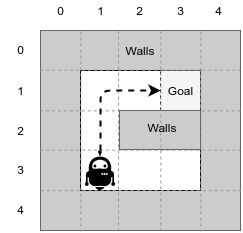
\includegraphics[width=0.4\textwidth]{./figures/asp_example}
\caption{5$\times$5 grid maze example (ASP planning)}
\label{environment_example}
\end{figure}
We use the same $5 \times 5$ grid maze as an example to highlight how the ASP planning works. 
Suppose that the agent is at (1,3) and has already found a terminal state (3,1).
Thus the agent can make an action plan to reach the goal. The ASP program for this example is provided as follows:

\lstinputlisting[
    caption  = {Example of ASP program},
    label = {list:asp_program_example}
]{asp_planning_example.pl}
The learnt hypotheses given by ILASP contain state transition for all four directions, and the agent has already seen necessary wall locations. The ASP program defined in Listing \ref{list:asp_program_example} returns the answer sets as a plan. By following the answer sets, the agent is able to reach the terminal state at (3,1).

\begin{equation*}
\begin{split}
&\textsf{state\_at((1,3),0),action(up,0),}\\
&\textsf{state\_at((1,2),1),action(up,1),}\\
&\textsf{state\_at((1,1),2),action(right,2),}\\ 
&\textsf{state\_at((2,1),3),action(right,3),}\\
&\textsf{state\_at((3,1),4).} 
\end{split}
\end{equation*}
\end{examp}
% Together with hypothesis, the background knowledge will used to solve for answer sets program. 
% However, since hypothesis is not complete, there is more than one answer set at each time step. 
% Since one of the answer sets state\_at is correct, the rest will be in the exclusions in the answer set, 
% which is used to further improve the hypothesis in the next iteration of inductive learning.
% In this example, the following is the answer set program
% The answer set using the hypothesis XXX is 
% The answer set using the improved hypothesis is XXX, 
% Which correctly returns a sequence of actions and predicted states.
% This incorrect plan is also a source for learning a better hypothesis. 
% As shown in Example XX, if the hypothesis is not a full hypotheses, outputs of ASP contain lots of \textsf{state\_at((X,Y), T)} at the same states. 
% Given the agent is at one state at each time step, these duplicates are all included in exclusions, as defined in Definition \ref{def:ILPRL_exc}.
% When the agent encounters a new environment (e.g a new wall), this new information will be added to its background, which will be used to improved the hypothesis. 
% Similarly, after executing an action by following the generated plan, the agent receives a new positive example. If the new positive example is not covered by the current hypotheses, 
% ILASP reruns using the new example to improve the hypotheses. 
% next time ILASP gets executed.
% For example,
% \begin{equation*}
% \begin{split}
% &\textsf{state\_at((1,1),1), action(right,1)}\\
% &\textsf{state\_at((2,1),2), action(right,2)}\\
% &\textsf{state\_at((3,1),3), action(right,3)}\\
% &\textsf{state\_at((4,1),4), action(right,4)}\\
% &\textsf{state\_at((5,1),5)}, \cdots
% \end{split}
% \end{equation*}
% At the start of the learning, H is usually not correct or too general, using this H will generate lots of answer sets that are not useful for the planning.
% These examples will be collected and included as exclusions of a new positive example.

\section{Exploration}
\label{exploration}
In this section, we explain the exploration policy of ILP(RL). While the agent can learn the hypotheses and execute a planning by interacting with the environment as shown in Figure \ref{fig:ILPRL_overview},
there are mainly two reasons why ILP(RL) requires exploration. 
First, the ILP(RL) agent can only do ASP planning only if it finds a terminal state. 
Therefore the agent needs to continues exploring the environment until it finds the terminal state. 
Second, even if the terminal state is found and the agent generates a planning based on the hypotheses and background knowledge, 
the plan does not guarantee that the agent always finds an optimal policy.
While the agent exploits what is already learnt and follow the best plan based on the current hypotheses and background knowledge,
the agent also needs to explore by taking a random action different in order to discover a new state, which might make the agent find an even shorter path and therefore higher total rewards in the long term.

One of the simple exploration policies in RL is called \textit{$\epsilon$-greedy policy}.
$\epsilon$-greedy policy states that an agent follows the optimal policy with probability of (1- $\epsilon$) where $\epsilon \in [0,1]$, 
and the agent takes a random action with probability of $\epsilon$. $\epsilon$ is a hyper-parameter and chosen externally.

When the agent deviates from the planning by taking an random action and moves to a new state, the agent generates a new planning from the new state. 
Since the ILP(RL) agent does not know when the optimal plan is found, it is necessary for ILP(RL) to continues $\epsilon$-greedy policy.
% Based on $\epsilon$-greedy policy in RL, we define the exploration policy for ILP(RL) in \ref{alg:exploration}:
% \begin{algorithm}[!htb]
% \caption{ILP(RL) Exploration Policy}
% \begin{algorithmic}[1]
% \label{alg:exploration}
% \renewcommand{\algorithmicrequire}{\textbf{Input:}}
% \State \textbf{Input:}
% \State \ \ \ \ \ \ Current state $s$
% \State \ \ \ \ \ \ Actions $A = \{ 1, ..., n\textsubscript{a}\} A: X \rightarrow A$
% \State \ \ \ \ \ \ Background knowledge for ASP $B$
% \State \ \ \ \ \ \ Current hypotheses $H$
% \State \ \ \ \ \ \ $\epsilon \in [0,1]$

% \Procedure{Policy}{$s, A, B, H, \epsilon$}
% \If {Terminal state is found}
% \State $A\textsubscript{plan} = Planning(s,B,H)$
% \State
% \LineComment{rand(0,1) generates a random number between 0 and 1}
% \If {$rand(0,1) < \epsilon $} 
% \space
% \State
% \LineComment{randInt(0,A) generates a uniformly random integer between 0 and $|A|$}
% \State $i = randInt(0, |A|)$ 
% \Return $a\textsubscript{i}$
% \Else \State $a\textsubscript{i}$ = $A\textsubscript{plan}(t)$
% \Return $a\textsubscript{i}$
% \EndIf
% \Else \State $i = randInt(1, |A|)$
% \Return $a\textsubscript{i}$
% \EndIf
% \EndProcedure
% \end{algorithmic}
% \end{algorithm}

\section{Implementation}
\begin{figure}[!htb]
\centering
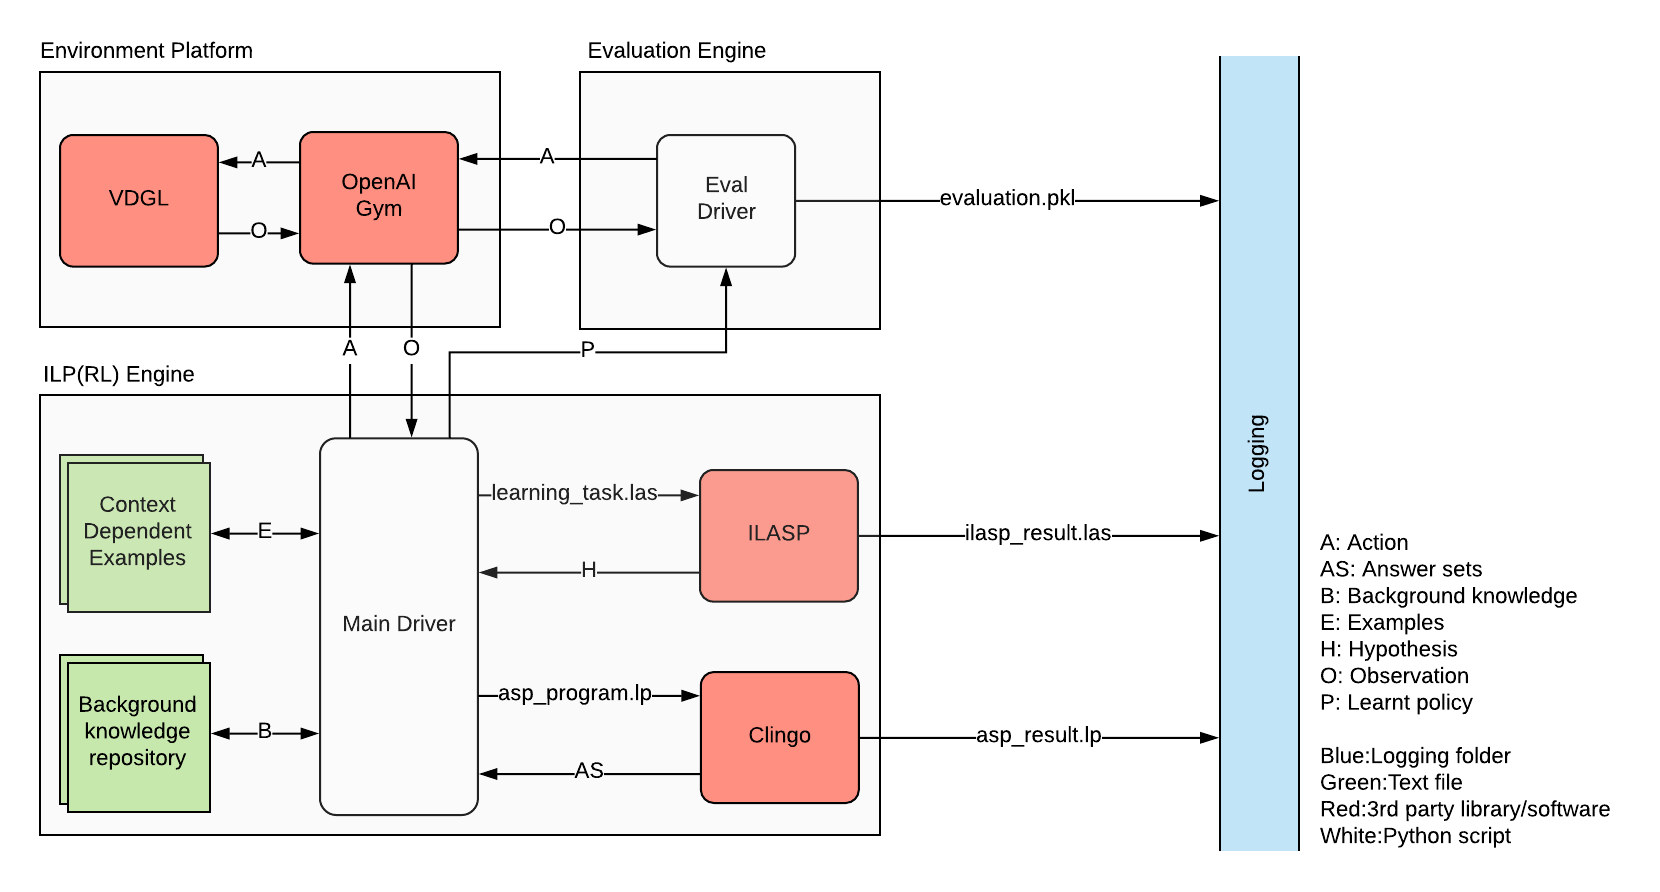
\includegraphics[width=1.0\textwidth]{./figures/ILPRL_dataflow}
\caption{Data flow diagram for ILP(RL) Engine, Environment and Evaluation components}
\label{fig:dataflow}
\end{figure}
We divide our implementation of the design outline into three separate software components: ILP(RL) Engine, Environment Platform and Evaluation Engine. The overview of our software implementation is shown in the data flow diagram in Figure \ref{fig:dataflow}. 

ILP(RL) Engine is our main framework explained in Chapter \ref{framework}. As shown in Figure \ref{fig:dataflow}, the main driver is written in Python and executes the algorithms, construct the necessary files and handles the communications by sending input and output among third-party software and libraries as well as executing their programs: ILASP, Clingo and the environment platform including the Video Game Definition Language (VDGL) and OpenAI Gym. The main driver is also responsible for I/O operation for context dependent examples as well as background knowledge, both are being accumulated in text files. Eval Driver is another Python script that executes the evaluation of ILP(RL) as well as benchmark RL algorithm, or Q-learning. The details of the evaluation is described in Chapter \label{evaluation}. All the results of inductive learning with ILASP, ASP planning and evaluation are recorded in Logging folder.
In the following sections, we explain how the main driver communicates with third-party softwaredetails.

\subsection{Inductive Learning with ILASP}
We use ILASP2i, an inductive learning system developed in \cite{Law2016b}.
ILASP2i is an iterative version of ILASP2, and is designed to scale with the numbers of examples. 
ILASP2i also introduces the use of context dependent examples.
The latest ILASP available is ILASP3, which is designed to work on a noisy examples. Our context dependent examples do not contain noise since they are all true state transition that the agent has experienced, and therefore ILASP2i was sufficient for our implementation.
which is discussed in Section XX. 
Although ILASP2i is designed to work with a large number of examples, inductive learning part is the bottleneck of our framework in terms of computational time. 
We did a number of optimisation in order to mitigate this. 

The first optimisation is the frequency of running ILASP. 
As already described in Algorithm \ref{algorithm:inductive_learning}, ILASP is ran only if the current hypothesis does not cover all the examples accumulated so far.

The next optimisation is through the command line. 
ILASP2i has a number of options, and we explain each option using the actual command we use to run ILASP

\begin{lstlisting}[]
    ILASP --version=2i FILENAME.las -ml=8 -nc --clingo5 
    --clingo "clingo5 --opt-strat=usc,stratify" 
    --cached-ref=PATH --max-rule-length=8
\end{lstlisting}

where,
\begin{itemize}
\item \textsf{--version=2i} specifies that we use ILASP2i.
\item \textsf{--ml=8} specified the maximum numbers of body that each rule can have. The default length is 3.
\item \textsf{--nc} means no constrains, and omits constrains from the search space. Since our target hypothesis is not a constraint, this option reduces the search space.
\item \textsf{--clingo5} generates Clingo 5 programs, which is faster, instead of Clingo 4.3.
\item \textsf{--clingo "clingo5 --opt-strat=usc,stratify"} specifies Clingo executable with the specified options. 
\textsf{usc, stratify} is unsatisfiable-core base optimisation with stratification using Gringo \cite{gringo}, a core XXX introduced in gringo version 3. REFERENCE.
\item \textsf{--cached-ref=PATH} enables the iterative mode, and keeps the output of the relevant example to a specified path, and start the learning from where it left before rather than going though all the examples.
\item \textsf{--max-rule-length=8} The default maximum number is 5.
\end{itemize}

\subsection{Planning with ASP}
Planning is computed using Clingo 5.

\begin{lstlisting}[]
    clingo5 --opt-strat=usc,stratify -n 0 FILENAME.lp
    --opt-mode=opt --outf=2
\end{lstlisting}

\begin{itemize}
\item \textsf{--clingo "clingo5 --opt-strat=usc,stratify"} specifies clingo executable with the specified options. 
\textsf{usc, stratify} is unsatisfiable-core base optimisation with stratification using Gringo \cite{gringo}, a core XXX introduced in gringo version 3. REFERENCE.
\item \textsf{-n 0} -n is an abbreviation of \textsf{models} to specify the maximum number of answer sets to be computed. \textsf{-n 0} means to compute all answer sets.
\item \textsf{--opt-mode=opt} computes optimal answer sets
\item \textsf{--outf=2} makes the output in JSON\footnote{http://json.org/} format
\end{itemize}

\subsection{Environment Platform}
\subsection{The Video Game Definition Language (VGDL)}

\begin{figure}[!ht!b]
\centering
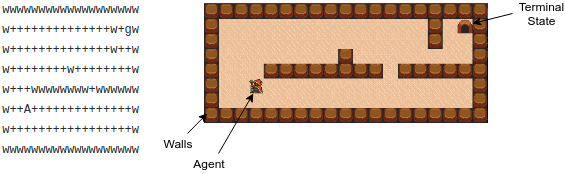
\includegraphics[width=1\textwidth]{./figures/env_sample}
\caption{Map sketch of a VGDL game (left) and it's high-level representation (right)} 
\label{VGDL_sample}
\end{figure}

We use the Video Game Definition Language (VGDL), which is a high-level description language for 2D video games providing a platform for computational intelligence research (\cite{schaul2013video}).
The VGDL allows users to easily craft their own environments, 
which makes us possible to do various experiments without relying on a default environment.

The base game we used to implement ILP(RL) is shown in Figure\ref{VGDL_sample}.
The map sketch is a plain text file and is easy to modify the configuration of the game.

\lstinputlisting[
    caption  = {VGDL description of a maze game},
    label = {list:vgdl}
]{vgdl.pl}

The behaviours of the game can be specified using VGDL as shown in \ref{list:vgdl}. 
All objects in the games can be described as a sprite in the \textit{SpriteSet}, where users can define the objects' properties.
\textit{InteractionSet} specify the effects of objects when two objects interact in the game.
\textit{TerminationSet} specify the conditions for ending the game.
The representation of each object can be specified in \textit{LevelMapping} and allows users to customise an original map.

We use PyVGDL\footnote{https://github.com/rubenvereecken/py-vgdl}, which is a high-level VGDL on top of pygame\footnote{https://www.pygame.org}, 
a Python modules designed for writing video games.

\subsection{OpenAI Gym}
\label{sebseq:openai_gym}
The VGDL platform provides an interface with OpenAI Gym (\cite{Brockman2016}), a commonly used benchmark platform for RL research.
The communication between VGDL environment and an agent, is through OpenAI Gym interface. 
\ref{list:openai} shows the functions provided by OpenAI Gym as well as the simple implementation for RL. 

In this report, an agent receives a reward of -1 for any state except the terminal state, and receives reward of +10 for the terminal state, or the goal.

% In all experiments, the agent receives -1 in any states except the goal state, where it gains a reward of 10.
% Once the agent reaches the goal, or termination state, that episode is finished and the agent start the next episode from the starting point.

\lstinputlisting[
  language = Python,
  caption  = {OpenAI gym interface},
  label = {list:openai}
]{openai.py}

\begin{itemize}
\item \textsf{env.reset()} resets the game and the agent starts from the starting position. We call it when the agent starts a new episode.
\item \textsf{env.step(action)} returns an observation of taking an action, which include the state location of the agent in terms of x and y coordinates, reward of the state, an boolean value indicating whether the agent reaches an terminal state.
The action is chosen by an RL algorithm of your choice. In the case of ILP(RL), action is chosen by the ASP planning or random exploration strategy between 0 and 3.
\item \textsf{env.render()} renders one frame of the environment to visualise the movement of the agent in pygame.
\end{itemize}


\chapter{Evaluation}
\label{evaluation}
In this Chapter, we conducted 4 different evaluations in simple maze environments to investigate how the ILP(RL) agent learns and finds the optimal policy.

\section{Experimental Setup}
\label{sec:experimental_setup}

\subsection{Evaluation Metrics}
\label{subsec:evaluation_metrics}

As introduced in Section \ref{sec:motivation}, our motivation is to improve the learning efficiency and capability of transfer learning in RL.
Therefore, these are the two main measurements for the performance of ILP(RL).
The learning efficiency is measured in three different ways: performance of optimal policy, convergence of inductive learning and runtime of ILP(RL). Due to the random exploration for both ILP(RL) and a benchmark, the performance of each experiment varies. Especially ASP planning of ILP(RL) starts only when the agent finds a terminal state and it is dependent on an random exploration. In order to smooth the impact of the randomness, we ran 30 experiments per evaluation and computed an average for all the evaluation metrics. Within an experiment, an agent is allocated 250 time steps per episode, 100 episode per experiment.

In order to compare the performance of ILP(RL) with an existing RL method, we use Q-learning as our base benchmark.
Q-learning is widely used RL technique, and given the environments used for the experiments are a simple environment in that
it is discrete and deterministic, this method is sufficient as a benchmark.

% TODO Q-leaning Implementation
% As defined in Algorithm XX (Q-learning) in Section \ref{td_learning_section}, we randomly 
% randomly initialise the state-action value functions except the terminal state, and we measure the same evaluation metrics as ILP(RL), 
% and compare the performance of the two algorithms in order to examine how well ILP(RL) learns faster than Q-learning.
% (Optimistic and pessimistic initialisation.)

\subsubsection{Performance of optimal policy}
The performance of ILP(RL) is compared with a benchmark in terms of
 optimal policy, which is measured in terms of the total reward that an agent gains per episode by following its optimal policy.
For all the evaluations, the agent receives -1 for any states except a terminal state and receives +10 when it reaches the terminal state.
For example, if an agent requires the minimum 10 actions to get to a terminal state, the maximum total reward that the agent could gain per episode is 0 (-1 reward at each action +10 for reaching the terminal state).

In RL analysis, the optimal policy is measured without exploration nor learning. For ILP(RL), for example, the agent might still take an random action even when the ASP planning is already optimal. Thus, the exploration policy does not allow us to measure the performance of it's optimal policy. Thus at after every episode, we disable an random exploration and inductive learning, and run the same experiment, so that the agent can only follow its optimal policy. In the case of ILP(RL), if the agent does not know a terminal state or hypothesis, it does not have any policy because ASP planning cannot be executed, and therefore the agent gets -250 total reward.
\subsubsection{Convergence of Inductive Learning}
The convergence of inductive learning is measured to see the learning curve of inductive learning phase in ILP(RL), which is specified as follows:
\begin{equation}
\begin{split}
\frac{\textsf{The cumulative number of ILASP calls per time step}}{\textsf{The total number of ILASP calls in all episodes}} \in [0,1]
\end{split}
\end{equation}
This gives a normalised convergence rate of inductive learning with the maximum 1. For example, if the total number of ILASP calls in all episodes is 10 and there is a ILASP call at time step 1 episode 1, it is recorded as 0.1. When there is another ILASP call at time step 2 episode 1 after the first ILASP call, it is recorded as 0.2. The 10th ILASP call in this evaluation is recorded as 1. 
\subsubsection{Runtime}
We recorded runtime of both ILP(RL) and a benchmark at each episode, and plot the cumulative runtime over episodes. For ILP(RL), we also recorded the average runtime of ILASP calls per evaluation. All the evaluations were conducted in Linux Operating System with Intel i7-6560U CPU and 8GB RAM.

\subsection{Parameters}
\begin{table}[!ht!b]
\centering
\begin{tabular}{lll}
\hline
Parameter            & ILP(RL)    & Q-learning      \\ \hline
The number of experiment per evaluation& 30       & 30       \\
The number of episode per evaluation& 100        & 100        \\
Time steps per episode& 250        & 250        \\
% Discount rate        & 0,5       & 1.4e-2       \\
$\alpha$ (learning rate)        & N/A       & 0.5       \\
$\epsilon$ (epsilon)         & 0.1        & 0.1        \\
Reward for any states except a terminal state  & -1        & -1       \\
Reward for a terminal state     & 10        & 10       \\
\end{tabular}
\caption{List of parameters used in the evaluations}
\label{table:parameter}
\end{table}

All the parameters used in the evaluations are summarised in Table \ref{table:parameter}.
We trained the agents with maximum 250 time step, 100 episodes, and conducted the same experiment 30 times in each environment. 
The number of time steps should be sufficient for the both algorithms to reach a terminal state by the $\epsilon$-greedy exploration strategy, 
which we specify 250 time steps for all experiments. 
The number of episode is specified such that both ILP(RL) and Q-learning eventually reaches the optimal policy.
Every episode starts from a starting state. If the agent reaches the terminal state within 250 time steps, the episode is complete and the next episode starts with the fixed starting state. 

The learning rate  $\alpha$ for Q-learning, as shown in Equation \ref{eq:q_learning}, determines how much Q-value is updated each time. Since our environments are relatively simple, we use 0.5 for $\alpha$. For the same reason, $\epsilon$ for both ILP(RL) and Q-learning is 0.1.

The rewards were arbitrarily assigned -1 for all states except the terminal state, and 10 for the terminal state.

We conducted 4 different evaluations using different environments to highlight each aspect of ILP(RL) algorithm.
\section{Learning Evaluation}
\label{sec:learning_evaluation}

\subsection{Evaluation 1: Baseline}
\label{subsec:experiement1_setup}

\begin{figure}[!htb]
\centering

\includegraphics[width=0.5\textwidth]{./figures/experiment1}
\caption{Game environment for Evaluation 1}
\label{fig:experiment1}
\end{figure}
    
The purpose of the first evaluation is to highlight how ILP(RL) agent learns the hypotheses using inductive learning and executes an ASP planning.
The environment is a simple maze where the terminal state is located the right upper corner as shown in Figure \ref{fig:experiment1}.
The shortest time step between the agent's starting state and the terminal state is 18 steps, thus the maximum total reward the agent could gain is -8.

\subsection{Evaluation 1: Result}
\label{subsec:experiment1_result}

\begin{figure}[!htb]
\centering
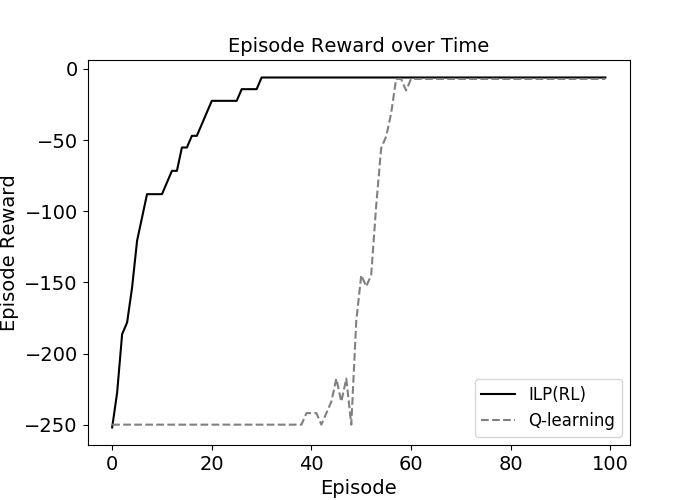
\includegraphics[width=0.7\textwidth]{./figures/experiment1_test}
\caption{Evaluation 1: optimal policy }
\label{experiment1_result}
\end{figure}

Figure \ref{experiment1_result} shows the performance of optimal policy.
ILP(RL) reaches the optimal policy faster than Q-learning: ILP(RL) reaches the optimal policy at before 40 episode, 
whereas Q-learning reaches the optimal policy at around 60 episode. ILP(RL) learns the optimal policy at an earlier episode because once the terminal state is found, the planning is always correct since there is only one way to reach the terminal state. The variations of the convergence to a optimal policy for ILP(RL) is dependent on how quickly the agent finds the terminal state. 
Since the exploration of ILP(RL) is based on $\epsilon$-greedy policy with the current ILP(RL), this result shows that there is a potential that a better exploration policy further improves the ILP(RL) learning.

The convergence of Q-learning for reaching an optimal policy is steeper than that of ILP(RL). This is because the state-action value functions are updated with the rate of $\alpha$, and the optimal policy for Q-learning is achieved when the optimal state-action value functions are achieved. By contrast, 
ILP(RL) gradually learns state transition of the environment using inductive learning and uses the background knowledge to accurately plan. 

Overall this result shows that ILP(RL) converges to the optimal policy faster than Q-learning in this simple scenario, achieving more data-efficient learning.

\lstinputlisting[
%   language = Prolog,
  caption  = {Hypotheses learnt in Evaluation 1},
  label = {list:experiment1_hypothesis}
]{experiment1_hypothesis.pl}

In addition to the data-efficient learning, what the agent has learnt with ILP(RL) is expressive.
Learnt hypotheses are shown in \ref{list:experiment1_hypothesis}, which are state transition for all directions, both when an adjacent state is a wall or not wall. The learnt state transitions are easy to understand for human users, and general in that they can be applied to a different similar environment.
The full learning task for this evaluation is in Appendix \ref{chap:learning_tasks_eval1}.

Next, we see how the agent learns the hypotheses over time. We plot part of the learning convergence for ILASP at episode 0 in Figure \ref{experiment1_ilasp}.
It converges to 1 after 200 episode, and shows that the agent learns the target hypotheses at the episode 0.
Since the two variables that the agent require to construct optimal answer set planning are the hypotheses and background knowledge, and the target hypotheses are learnt at episode 0, the convergence of finding an optimal policy for ILP(RL) is dependent on how quickly the agent finds a terminal state. 

\begin{figure}[!htb]
\centering
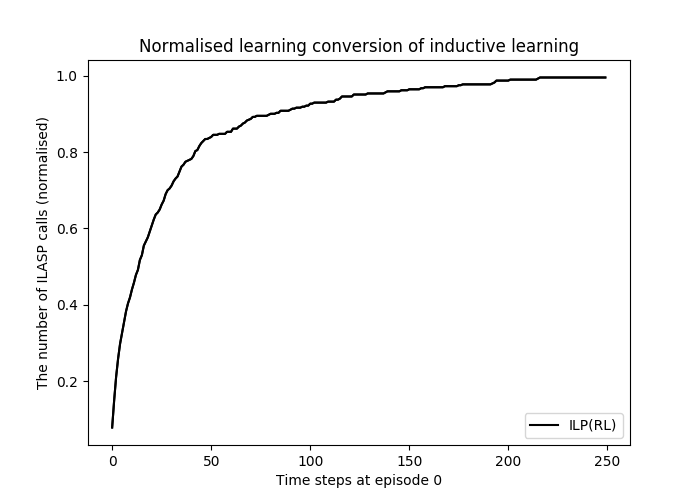
\includegraphics[width=0.7\textwidth]{./figures/experiment1_ilasp}
\caption{Normalised learning convergence by ILASP for experiment 1}
\label{experiment1_ilasp}
\end{figure}

Finally, we compare the runtime of two algorithms. 
The Figure \ref{exp1_runtime} shows that the runtime of ILP(RL) in the first few episodes is significantly high. 
This is due to the fact that ILP(RL) runs ILASP calls to learn the hypotheses at the beginning of episodes.
The Figure \ref{exp1_runtime} therefore highlights an issue that inductive learning is likely the bottleneck in terms of computational time.
This issue may not be critical in cases where the time of the time between the time steps is not an issue. If the performance is measured in terms of computation time rather than the number of iterations, 
ILP(RL) does not perform better than Q-learning. 
The average runtime of inductive learning is 5.58 seconds, and there are on average 12.83 times inductive learning per episode in this environment.
% RUNTIME FOR ILASP: 5.579039041812603
% ILASP RUNS TOTAL: 12.83 times
The ASP planning is not a bottleneck of ILP(RL), but still takes longer time than Q-learning, as can be observed by the divergence of cumulative runtime between the two algorithms. 
This experiment show that while ILP(RL) learns faster than Q-learning in terms of the number of episodes, it suffers from increasing computational time due to inductive learning as well as ASP planning.

\begin{figure}[!htb]
\centering
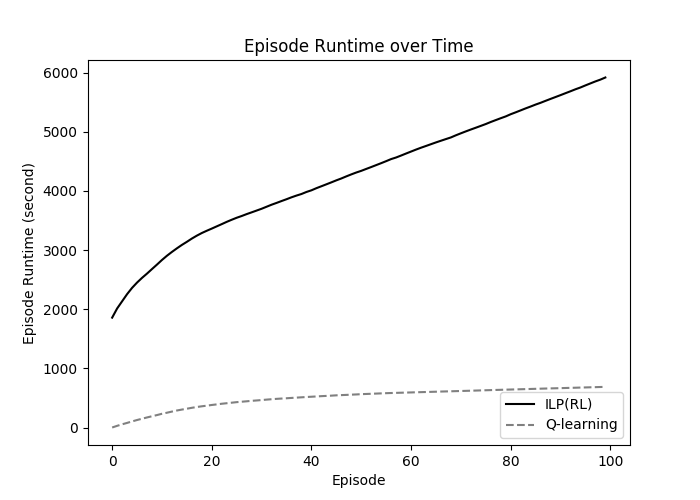
\includegraphics[width=0.7\textwidth]{./figures/experiment1_runtime}
\caption{Evaluation 1: runtime comparison}
\label{exp1_runtime}
\end{figure}

\subsection{Evaluation 2: Extended Baseline}
\label{subsec:experiement2_setup}

\begin{figure}[!htb]
\centering

\includegraphics[width=0.5\textwidth]{./figures/experiment2_setup}
\caption{Game environment for Evaluation 2}
\label{experiment2}
\end{figure}
Evaluation 2 was conducted to see if the agent learns a teleport and finds an optimal path using the teleport. The environment is the same as Evaluation 1 except the presence of teleport link and three extra walls to surround the destination teleport.
In the environment shown in Figure \ref{experiment2},
there are two ways to reach the goal: using a floor path to reach the goal located on the top right corner, or using the teleport.
The environment is designed such that using the teleport is a shorter path and therefore gives a higher total reward.
Compared to Evaluation 1, two extra language biases are added as follows:
\begin{equation*}
\begin{split}
&\textsf{\#modeb(1, link\_start(var(cell)), (positive)).}\\
&\textsf{\#modeb(1, link\_dest(var(cell)), (positive)).}
\end{split}
\end{equation*}

\textsf{link\_start(var(cell))} is a state for departure of the teleport and \textsf{link\_dest(var(cell))} is the destination of the teleport. 
The teleport link is one-way: \textsf{link\_start} takes the agent to \textsf{link\_dest}, but \textsf{link\_dest} does not take the agent back to \textsf{link\_start}.
This extra types allows ILASP to learn additional hypotheses.
The full learning task for this evaluation is in Appendix \ref{chap:learning_tasks_eval2}.

Also \textsf{link\_start} and \textsf{link\_dest} need to be stored in background knowledge rather than as context dependent examples when the agent finds them, 
because ILP(RL) needs to generate exclusions regarding the teleport link behaviour.
The link locations need to be available for all positive examples so that ILASP correctly learns different a valid move for floor and teleport.

Because of the teleport link, the shortest path is 13 steps to reach the terminal state. Thus the maximum total reward that the agent could gain is -3.

\subsection{Evaluation 2: Result}
\label{subsec:experiment2_result}
    
\begin{figure}[!htb]
\centering
% 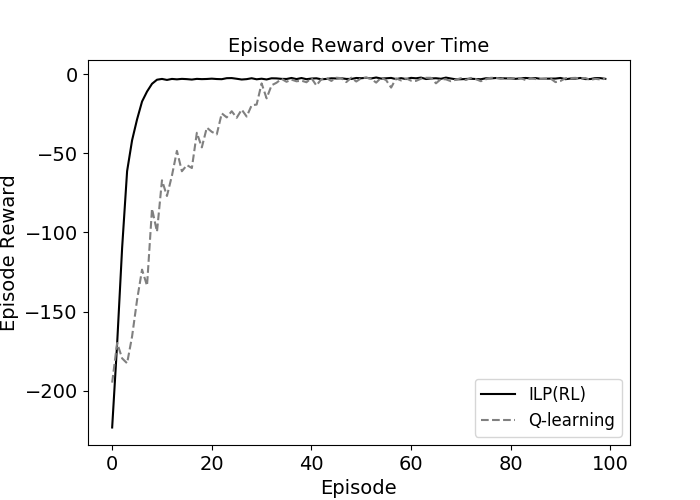
\includegraphics[width=0.55\textwidth]{./figures/experiment2_training}
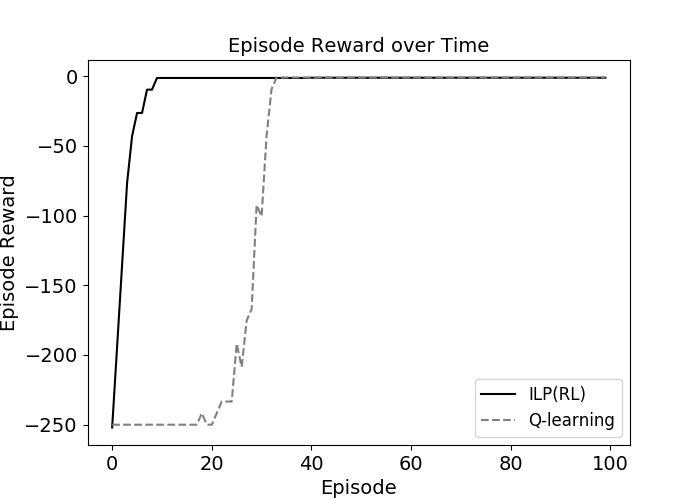
\includegraphics[width=0.7\textwidth]{./figures/experiment2_test}
\caption{Evaluation 2: optimal policy}
\label{experiment2_training}
\end{figure}

Similar to Evaluation 1, as shown in Figure \ref{experiment2_training}, ILP(RL) finds an optimal policy faster than Q-learning. Compared to the environment in Evaluation 1, ILP(RL) finds an optimal policy at earlier episode, because finding a terminal state is easier for ILP(RL) in this environment, since finding \textsf{link\_start} immediately leads the agent to the terminal state rather than having to go through a floor path to the upper right corner of the environment.
\newpage
\lstinputlisting[
  caption  = {Incomplete hypotheses for Evaluation 2},
  label = {experiment2_hypothesis_intermediate}
]{experiment2_hypothesis_intermediate.pl}

To highlight the inductive learning process of the new concept of teleport link, Listing \ref{experiment2_hypothesis_intermediate} is an intermediate incomplete hypotheses learnt by ILASP.
These hypotheses are generated just after the agent steps onto the \textsf{link\_start}. However, the first hypothesis in Listing \ref{experiment2_hypothesis_intermediate} states that
when \textsf{link\_dest} is available \textsf{state\_after} is true. Since \textsf{link\_dest} is available in background knowledge rather than context in the context dependent examples,
when solving for answer sets to generate a plan, it generates incorrect \textsf{state\_after} at every time step.

However, as shown in Definition \ref{def:ILPRL_exc}, these generated \textsf{state\_after} are all incorrect and therefore will be added to exclusions of the next positive example.
These exclusions will later refine hypotheses and the final complete hypotheses are shown in Listing \ref{list:exp2_final_hypotheses}.

\lstinputlisting[
  caption  = {Complete hypotheses for Evaluation 2},
  label = {list:exp2_final_hypotheses}
]{experiment2_hypothesis.pl}

Compared to the Evaluation 1, there are two new hypotheses due to the presence of the teleport links.
These learnt hypotheses are also applicable to an environment where there is no teleport links, such as the environment in Evaluation 1.
In this case, the first two hypotheses in Listing \ref{list:exp2_final_hypotheses} are never be used 
since the body predicates relating to link\_start(V0), link\_dest(V1) are never be satisfied.

\begin{figure}[!htb]
\centering
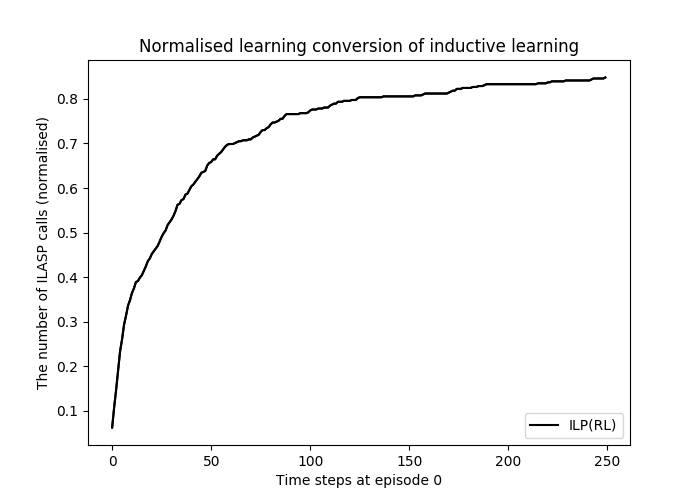
\includegraphics[width=0.7\textwidth]{./figures/experiment2_ilasp}
\caption{Normalised learning convergence by ILASP for Evaluation 2}
\label{experiment2_ilasp}
\end{figure}

Figure \ref{experiment2_ilasp} shows the learning convergence of inductive learning at episode 0.
Similar to Evaluation 1, most of ILASP calls occur at the beginning of the episode, as shown in Figure \ref{experiment2_runtime}.
The results of Evaluation 1 and 2 confirm that ILP(RL) learns state transition at the beginning of learning.
If the agent finds the teleport link state at a later episode, ILP(RL) refines the hypotheses by learning a new state transition regarding the teleport link.

\begin{figure}[!htb]
\centering
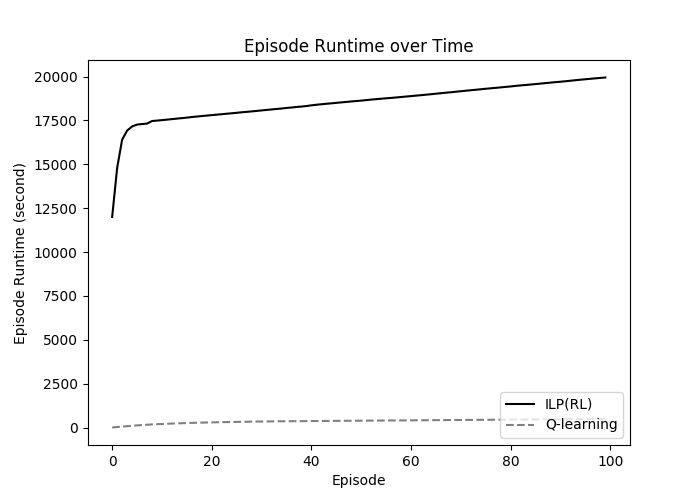
\includegraphics[width=0.7\textwidth]{./figures/experiment2_runtime}
\caption{Evaluation 2: runtime comparison}
\label{experiment2_runtime}
\end{figure}

Figure \ref{experiment2_runtime} shows the runtime of ILP(RL) and Q-learning in Evaluation 2. 
Despite the fact that the size of the environment is the same as Experiment 1,
there is a significant increase of runtime for ILP(RL) at the beginning of episode. 
This is because of the increase of search space in order for ILP(RL) to learn a new state transition.
The average runtime of inductive learning is 95.47 seconds, and there are on average 16.23 times inductive learning per episode.
% RUNTIME AVERAGE: 95.47274640401204
% RUNTIME COUNTS: 16.233333333333334
\begin{table}[!ht!b]
\centering
\begin{tabular}{lll}
\hline
Metrics            & Evaluation1    & Evaluation2      \\ \hline
Average ILASP runtime time (seconds)& 5.58        & 95.47       \\
The number of ILASP calls &  12.83      & 16.23      \\
Search space &  1690      & 32755       \\
\end{tabular}
\caption{Comparison of runtime, ILASP calls and search space between Evaluation 1 and 2}
\label{table:runtime_comparison}
\end{table}

To highlight the increase of runtime, Table \ref{table:runtime_comparison} summarises the comparison of runtime, ILASP calls and search space between Evaluation 1 and 2. 
Because of the two extra language biases for learning the teleport link, the search space in Evaluation 2 is significantly larger than that of Evaluation 1. This increase affects each ILASP call, resulting in much longer ILASP runtime in Evaluation 2. ILP(RL) calls ILASP an average of 3.4 more times in order to learn new hypotheses regarding the teleport link state.

While ILP(RL) still learns faster than Q-learning in terms of the number of iterations, 
the result of Experiment 2 shows that, the learning time per episode increases with respect to the size of search space, 
which corresponds to the number of state transition that the agent needs to learn in the environment.

\section{Transfer Learning Evaluation}
\label{sec:transfer_learning_evaluation}

\subsection{Evaluation 3: Transfer Learning}
\label{subsec:experiement3_setup}

\begin{figure}[!htb]
\centerline{

\includegraphics[width=0.5\textwidth]{./figures/experiment3_before}
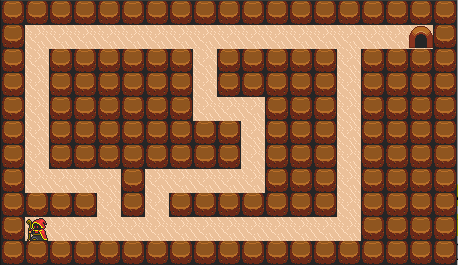
\includegraphics[width=0.5\textwidth]{./figures/experiment3_after}
}
\caption{Game environment for Evaluation 3: before (left) and after (right) transfer learning}
\label{experiment3_setup}
\end{figure}

In Evaluation 3, we investigate the possibilities of transfer learning between similar environments.
We trained the ILP(RL) agent using the environment on the left in Figure \ref{experiment3_setup}, 
and transfer the learnt hypotheses as well as context dependent examples to a new environment on the right in Figure \ref{experiment3_setup}. The terminal state is located at the same location, and there is an extra path in the environment on the right of Figure \ref{experiment3_setup}.

Context dependent examples are transferred to the new environment. This is because if there is a new hypothesis that the agent needs to learn in the new environment, 
ILP(RL) needs to refine the hypothesis using these transferred context dependent examples. Thus all the context dependent examples are also transferred as well as the learnt hypotheses. 

Background knowledge is not transferred since the wall locations are different in a new environment.
The agent therefore starts the exploration of the new environment with an empty background knowledge and gradually collects them over time.
The terminal state is the same as that in the first environment, but the shortest path to the goal is different between the two environments as new shorter path is introduced in the right environment in Figure \ref{experiment3_setup}.

In addition to Q-learning, we use three extra agents for comparison as follows. 

\begin{itemize}
    \item Agent(TL): The agent with transferred hypotheses, examples and also remembers the location of the terminal state.
    \item Agent(noTL)\textsubscript{Goal}: The agent with no transferred information, but knows the location of the terminal state.
    \item Agent(noTL)\textsubscript{noGoal}: The agent with no transferred information, including the location of the terminal state.
\end{itemize}

\lstinputlisting[
%   language = Prolog,
  caption  = {Hypotheses for Evaluation 3},
  label = {exp3_hypotheses}
]{experiment3_hypothesis.pl}

Listing \ref{exp3_hypotheses} is the hypotheses that is transferred to a new environment, which is acquired by training the agent in the environment once on the left of Figure \ref{experiment3_setup}.
The learnt hypotheses are the same hypotheses are that in Evaluation 1 shown in Listing \ref{list:experiment1_hypothesis} in the environment, they are a general concept that is applicable to any similar environments.

\subsection{Evaluation 3: Result}
\begin{figure}[!htb]
\centering
% 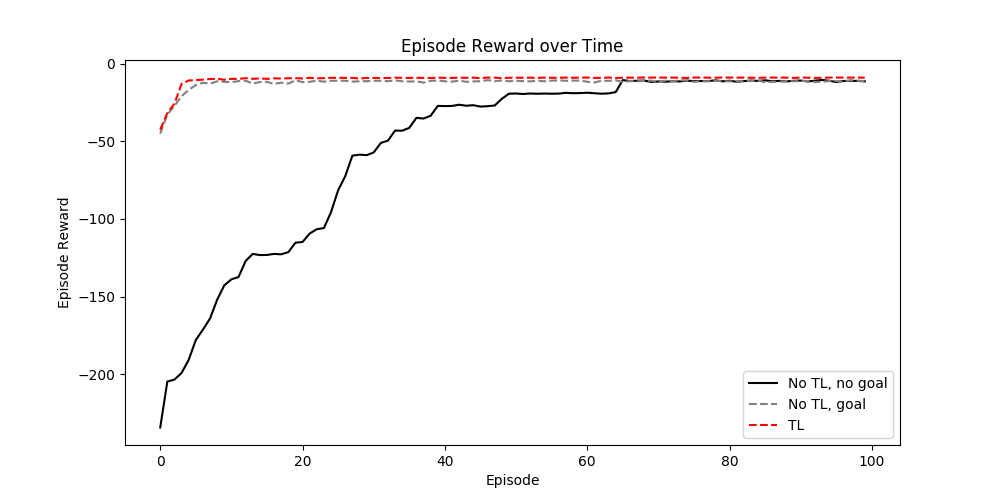
\includegraphics[width=0.55\textwidth]{./figures/experiment3_after_training}
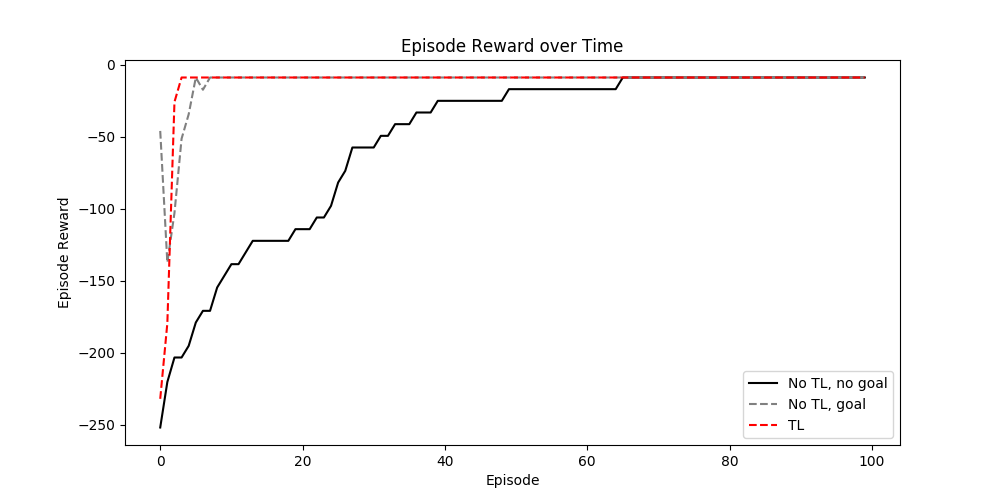
\includegraphics[width=0.7\textwidth]{./figures/experiment3_after_test}
\caption{Evaluation 3: optimal policy}
\label{experiment3_training}
\end{figure}

The result is shown in Figure \ref{experiment3_training}.
For Agent(TL), since the complete hypotheses are already known to the agent as well as the terminal state, the agent can do ASP planning from episode 0. There is no ILASP calls in the new environment since the transferred hypotheses are already the target hypotheses and cover all the examples the agent encounters in the new environment.
The only information required is background knowledge for the ASP planning, namely the locations of the walls, which are quickly acquired and reached the maximum total reward at the very beginning of episodes.

The next best agent in terms of convergence rate is Agent(noTL)\textsubscript{Goal}. Since the terminal state is known to the agent, 
the agent can do the planning from episode 0. However, the agent needs to learn the hypotheses. The reason that the convergence rate is almost the same as that of Agent(TL) is that, the ILP(RL) learns the complete hypotheses at very early episode, as observed in Evaluation 1 and 2. 
Thus there is no difference between Agent(TL) and Agent(noTL)\textsubscript{Goal} in terms of learning speed. 

What makes a difference for finding an optimal policy is whether the agent knows the terminal state, which can be seen by compering between Agent(noTL)\textsubscript{Goal} and Agent(noTL)\textsubscript{noGoal}.
The difference in terms of the iterations is that Agent(noTL)\textsubscript{noGoal} needs to find the terminal state first before starting the planning, which is a random exploration.

The capabilities of the transfer learning works especially when the terminal state is transferred, because the ASP planning of ILP(RL) depends on the terminal state. 
In addition, this evaluation further confirms that there is a promising potential for improving the exploration strategy to find the terminal state as soon as possible.

\subsection{Evaluation 4: Extended Transfer Learning}
\label{subsec:experiement4_setup}
\begin{figure}[!htb]
\centerline{
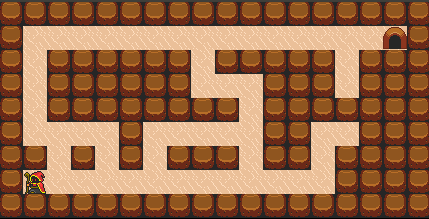
\includegraphics[width=0.5\textwidth]{./figures/experiment4_before}

\includegraphics[width=0.5\textwidth]{./figures/experiment4_after}
}

\caption{Game environment for Evaluation 4: before (left) and after (right) transfer learning}
\label{experiment4_setup}
\end{figure}
In Evaluation 4, we trained ILP(RL) on the left in Figure \ref{experiment4_setup}, and transferred context dependent examples as well as the learnt hypotheses. The objective of this experiment is to see how the transferred agent learns a new state transition on top of the transferred hypotheses. In the new environment on the right of Figure \ref{experiment4_setup}, there is a teleport link and using the teleport is the shortest path to the terminal state. 
This is a new concept that did not exist in the trained environment and therefore the agent needs to learn it after the hypotheses are transferred.
The same as Evaluation 3, we use four different agents.

\subsection{Evaluation 4: Result}
\label{subsec:experiment_result_4}

\begin{figure}[!htb]
\centering
% 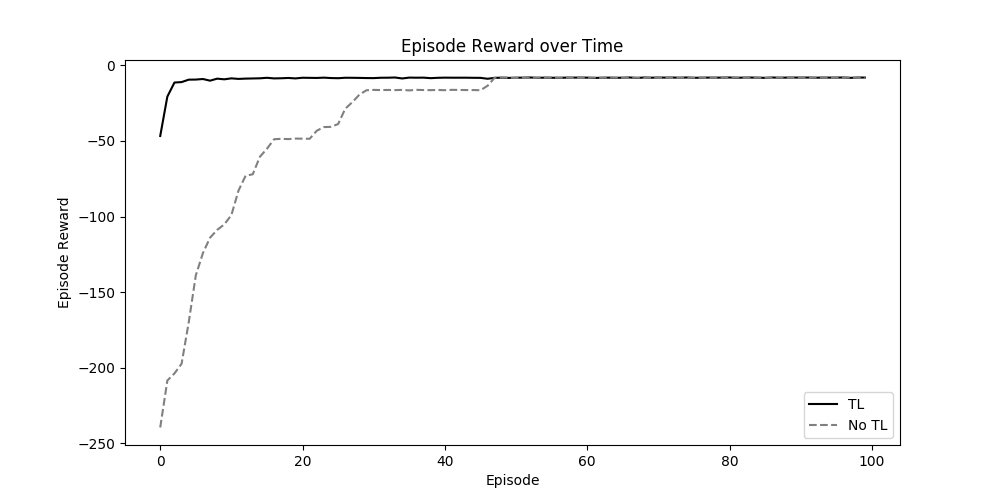
\includegraphics[width=0.55\textwidth]{./figures/experiment4_training}
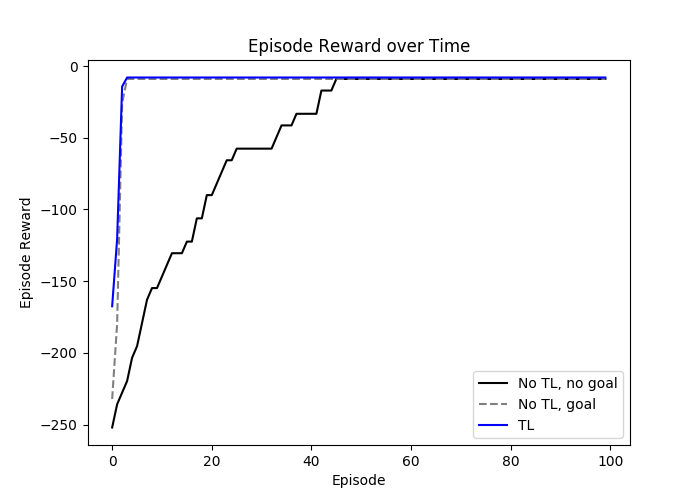
\includegraphics[width=0.7\textwidth]{./figures/experiment4_test}
\caption{Evaluation 4: optimal policy}
\label{experiment4_training_test}
\end{figure}

Figure \ref{experiment4_training_test} shows the results of optimal policy. 
Agent(TL) is able to successfully learn the new concept and quickly finds the optimal policy at the early episodes. Similar to Evaluation 3, Agent(notTL)\textsubscript{Goal} also quickly reaches the optimal policy,  
This experiment shows that the hypotheses is transferable even in cases where there is a new hypothesis the agent needs to learn in a new environment.

Also the difference of the state where the link is located does not cause any problems with ILP(RL) algorithm even when the positive examples in the previous environment are transferred. This is because information of ajacent walls are within the context of each example rather than background knowledge. This experiment shows the flexibility of context dependent examples in RL senarios.

The new hypotheses the agent learns are the same as that of Evaluation 2. The hypotheses regarding \textsf{link\_start} and \textsf{link\_dest} is what the Agent(TL) learnt in the new environment.

\section{Discussion}
\label{sec:discussion}

We evaluated the properties of ILP(RL) using simple maze environments. While the development of ILP(RL) is still in early stage and only a proof-of-concept, we observe both strengths as well as weakness of the current framework of ILP(RL). We summarise both of these in the following sections.

\subsection{Strengths of ILP(RL)}
As observed in the 4 evaluations, there are several advantages of ILP(RL) over Q-learning.

\begin{description}
\item[Faster learning of an optimal policy]
The ILP(RL) agent learns the general state transitions of the environment at the very early stage of learning, mostly at episode 0, and as soon as it finds the terminal state, is able to generate an ASP plan as a sequence of actions to find an optimal policy.
While this is a proof-of-concept approach, this way of RL is a new and the experiments show that this is a promising direction of the research.

\item[Transfer Learning]
Unlike existing RL algorithms, where it learns value functions or Q values, ILP(RL) learns a valid move as a hypotheses, which can be applied to similar but different environments.
We confirmed the possibility of transfer learning with the evaluations. Especially when the goal is known to the agent in Evaluation 3 and 4.
While this is a limited transfer learning since the terminal state is known in advance, this is still a useful transfer in cases where the terminal state is the same but the rest of the environment changes.
We also observed that the agent can learn a new hypothesis on top of the transferred hypotheses, which is very flexible in terms of applicability of the learnt hypotheses.

\item[Symbolic learning]
Since both the outcomes of ASP planning and inductive learning can be expressed in ASP syntax, the learning process as well as outcomes of ILP(RL) are easy to understand for human users, and the learnt hypotheses are very general state transitions of an environment.
\end{description} 

% The full hypotheses were learnt in the very early phase of learning and exploration phase. Thus with sufficient exploration, the model of the environment is correct
% and therefore it is able to find the optimal policy/path. 

% We show that ILP(RL) is able to solve a reduced MDP where the rewards are assumed to be associated with a sequence of actions planned as answer sets.
% Although this is a limited solution, there is a potential to expand it to solve full MDP as discussed in Further Research. 

\subsection{Limitations of the current framework}
\label{subsec:limitations}
Although the this first version of the ILP(RL) using inductive learning and ASP planning show potentials for a new way of solving RL problems, it is a proof-of-concept and there are a number of limitations with the current framework.
Some of these limitations are further elaborated in Further Research in Chapter \ref{sec:further_research}.

\begin{description}
\item[Runtime]
While we show that ILP(RL) converges to a optimal policy in terms of the number of episodes, the computational time is significantly longer than that of Q-learning due to the computation required for inductive learning with ILASP as well as ASP planning.
This limitation indicates that ILP(RL) may not be suitable in an environment where the runtime of learning is also a concern. ILP(RL) may also be unsuitable in an environment where there are moving objects based on time rather than time steps.

\item[Scalability issue for more complex environment]
ILP framework is known to be less scalable. The current framework is tested in a relatively simple environments, 
and proven to be work better than Q-learning in terms of learning an optimal policy by time. However, learning runtime of ILP(RL) in each time step is slower than that of Q-learning, which is worsen when there are more hypotheses that ILP(RL) needs to learn.
For example, as shown in Evaluation 1 and 2, adding two language bias significantly increased the runtime of the algorithm, since the search space grows significantly with respect to the language bias.
Whereas Q-learning updates value function regardless of whether there is a new concept such as teleport links, ILP(RL) needs to expands search space of hypotheses by adding more language bias. This is an important issue since many of RL research are focused on the development of RL algorithms in more complex environments.

Another question is the possibility of extending ILP(RL) to more realistic scenarios. RL works in more complex environments such as 3D or real physical environment, 
whereas the observations of an environment need to be expressed as ASP syntax for ILP(RL) to work.
\item[Requirements of assumptions]
ILP(RL) requires initial assumptions such as background knowledge or specification of language bias for search space. While most of existing reinforcement learning works in different kinds of environment without any pre-configuration, As shown in the Evaluation 2, it was necessary to add two extra modeb before learning starts.
Thus the current framework of ILP(RL) is unfeasible in cases where these learning concepts were unknown or difficult to define with language bias.

In addition, not only it needs search space, but also it is assumed that an agent knows the definition of adjacent state and is able to see the adjacent states. 
While this assumption may be reasonable in many cases, this is not common in traditional RL setting.

\item[solving limited MDP]
The current ILP(RL) framework does not make use of rewards for inductive learning and only uses the terminal state for ASP planning. While our evaluations were conducted in a simple environment and we assumed that there is only one reward for any states except a terminal state. As described in Section\ref{model_base_model_free_subsection}, other model-based RL methods learn a model of an environment, which tells the agent the reward and state transition functiosn. However, the current ILP(RL) only learns state transition and does not learn reward functions. In addition, some MDP problems contain no terminal state and instead there may be a different means to gain rewards. 
Since the current ILP(RL) is dependent on finding a terminal state for planning rather than maximising total rewards, 
the application of the current framework is limited to a particular type of MDP problem.

\end{description}  

Some of these issues are further discussed in Chapter \ref{conclusion}.



\chapter{Related Work}
\label{related_work}
In this section, we review related work in logic programming, reinforcement learning combined with ASP, symbolic RL, and some model-based RL, in order to motivate our new approach.
relational reinforcement learning.

The combination of inductive logic programming and reinforcement learning has its root in relational reinforcement learning. 

The combining logic-based learning with reinforcement learning has its roots in what is called relational reinforcement learning (RRL) \cite{Dzeroski2001}. 

RRL equipped with generalisation of inductive logic programming. 

RRL is based on first-order logic, and does not cope with negation as failure or non-monotonic reasoning.

However, most RRL algorithms focus on planning. 
RRL incorporates relational representations of states and actions to generalise Q-function and 
More recent work on using relational representation in RL is the paper in XX, which combines RRL and DRL in order to overcome the interpretability and an ability to generalise of DRL.
The proposed architecture uses self-attention mechanism to reason about the relations between entities in the environment to help improving policy. 
While RLL was applied to XX, this approach also shows an promising direction of using ILP in RL.

% reuse of experiences.

 \cite{Garnelo2016} introduced Deep Symbolic Reinforcement Learning (DSRL), a proof of concept for incorporating symbolic front end as a means of converting low-dimensional symbolic representation into spatio-temporal representations, which will be the state transitions input of reinforcement learning. 
 DSRL extracts features using convolutional neural networks (CNNs) \cite{LeCunL1998} and an auto-encoder, which are transformed into symbolic representations for relevant object types and positions of the objects. 
 These symbolic representations represent abstract state-space, which are the inputs for the Q-learning algorithm to learn a policy on this particular state-space. 
 DSRL was shown to outperform DRL in stochastic variant environments.
However, there are a number of drawbacks to this approach. 
First, the extraction of the individual objects was done by manually defined threshold of feature activation values, given that the games were geometrically simple. 
Thus this approach would not scale in geometrically complex games. 
Second, using deep neural network front-end might also cause a problem. As demonstrated in \cite{Su2017}, a single irrelevant pixel could dramatically influence the state through the change in CNNs.
In addition, while proposed method successfully used symbolic representations to achieve more data-efficient learning, 
there is still the potential to apply symbolic learning to those symbolic representations to further improve the learning efficiency, which is what we attempt to do in this paper.
\cite{Garcez2018} further explored this symbolic abstraction approach by incorporating the relative position of each object with respect to every other object rather than absolute object position. 
They also assign priority to each Q-value function based on the relative distance of objects from an agent.

\cite{Zambaldi2018} added relational reinforcement learning, a classical subfield of research aiming to combining reinforcement learning with relational learning or Inductive Logic Programming,  which added more abstract planning on top of DSRL approach. 
The new mode was then applied to much more complicate game environment than that used by \cite{Garnelo2016}.
%They incorporated a deep RL with architectural inductive biases
%structured representations of the game, and relatioal reasoning.
%The use of symbolic representations to achieve data-efficient learning was traditionally discussed in relational reinforcement learnign (RLL).
This idea of adding planning capability align with our approach of using ILP to improve a RL agent. 
We explore how to effectively learn the model of the environment and effectively use it to facilitate data-efficient learning and transfer learning capability.

%Transparency and interpretable capability of the model is another important aspect for machine learning applications.
%The history of data-efficient learning

Another approach for using symbolic reinforcement learning is storing heuristics expressed by knowledge bases [\cite{Apeldoorn2017}).  
An agent learns the concept of \textit{Hierarchical Knowledge Bases (HKBs)} (which is defined in more details in \cite{Apeldoorn2016} and \cite{Apeldoorn}] at every iteration of training, which contain multiple rules (state-action pairs). 
The agent then is able to decide itself when it should exploit the heuristic rather than the state-action pairs of the RL using  \textit{Strategic Depth}. 
This approach effectively uses the heuristic knowledge bases, which acts as a sym-symbolic model of the game.

Another field related to our research is the combining of ASP and RL. 
The original concept of combining ASP and RL was in \cite{Ferreira2017}, where they developed an algorithm that efficiently finds the optimal solution of an MDP of non-stationary domains by using ASP to find the possible trajectories of an MDP. 
ASP is used to find a set of states of an MDP as choice rules describing the consequences of each possible action.
% In order to find stationary sets, an extension of ASP called BC\textsuperscript{+}, an action language, was used. BC\textsuperscript{+} can directly translate the agent's actions into ASP form, and provide sequences of actions in answer sets.
The more details of theoretical explanation of this approach is described in XX.
This approach focused more on efficient update of the Q function using ASP, and does not make use of inductive learning.

Similar works were conducted for learning XX in PAPER, for XX in XXX and for XX in XX. 
All of them are based on experiment in using robot.


Our framework focus on ASP-based ILP with RL, which has not been explored.


\cite{Meadows2018} proposed an architecture for interactively discovering previously unknown axioms using reinforcement learning.
Axioms represent domain dynamics of preconditions and expected outcomes, as well as the relationship among actions of the agents and objects in the domain.
These discovered axioms are used to generate more general axioms that can be use for subsequence reasoning.
uses ASP program to encode a decision tree induction as well as relational representation in order to . 
The extension of [] is

%Incorporation of logic into reinforcement learning dates back to the study of relational reinforcement learning,

%There are a number of research conducted in applying DNN to symbolic reasoning.
%[From GamePlay to Symbolic Reasoning]


\chapter{Conclusion}
\label{conclusion}
\section{Summary of Work}
\label{sec:summary_of_work}

In this paper, we developed a new RL algorithm by applying ILP to develop a new learning process.
We summarise some of the works we have done throughout the project.

\begin{itemize}
\item We started off by looking at existing symbolic reinforcement learning approaches to understand the research fields and see the potentials of improving further researches.
Due to advances of ASP-based ILP frameworks and there is no existing works of applying ASP-based ILP into RL scenarios, this motivates us to pursuing the potentials of ILP to solve RL problems.
Because of the flexibility and expertise of ILASP, we decided to apply ILASP as our core learning framework.

\item We considered the target hypotheses and how to construct learning tasks. Our target learning is a valid move of the agent, and which can be expressed with state transition for each action.
Also all the components of learning tasks have to be in ASP-syntax, we developed a Python engine for translating all output of the environment into ASP-syntax.

surrounding information

\item As a way to use our learnt hypotheses to execute a sequence of actions, we used the Clingo ASP solver for our plan execution. 
The use of ASP optimisation is based on the assumption that the goal of the game is to find a shortest path to a terminal state.

\item We considered which kind of RL problems we would like to test with our new framework. Since this is a new proof-of-concept and testing core concepts were required, we chose a custom-maze game provided by VDGL and created original environments.

\item We tested our new framework in a various maze environments to highlight each aspect of the algorithm. We show that ILP(RL) learns faster than benchmarks for finding a shortest path, and show a capability of transfer learning.
While the experiments were conducted in a simple limited conditions, we show some promising potentials of the ILP-based approach for RL problems.

\end{itemize}

We used a latest ILP algorithm called ILASP, Learning from Answer Set Program to iteratively improve hypotheses.

\section{Further Research}
\label{sec:further_research}

Since the development of ILP(RL) is a new attempt and we only develop the initial version and tested only on simple maze games, 
there are a number of directions for further research. We discuss some of the possible improvements and further research in this section.

% More general transfer learning.
% Only empirically correct, no theoretically guarantee
% Our approach is similar to experience replay ??
% More promising approach is to combine RL algorithm and using ILP approach to complement each other, rather than replacing the bellman equation altogether. 
\begin{description}
    \item[Better exploration strategy]
    We used a random exploration strategy for both algorithms in order to compare the performance of ILP(RL) with existing RL algorithms. 
    As shown in the experiments, however, the convergence of ILP(RL) is heavily dependent on finding a terminal state in order to start planning part.
    In RL research, exploration strategy is another active research field and a more sophisticated exploration strategy would facilitate the learning of ILP(RL)
    such as Boltzman approach, Count-based and Optimistic Initial value TODO REFERENCE).
    % The current framework simply uses a simple random exploration, therefore even if the agent takes an random action and goes to a different state other than the planed one, 
    % the agent does the replan from the new state and quickly correct to the original plan path. 
    % This means it is likely that the agent of ILP(RL) only explores the adjacent cells and if there is a shorter path or new state
    % In other words, if the shorter path is far from the current state, the agent is unlikely be able to find the new state unless epsilon value is very high. 
    \item[Experiments on different environments]
    Since the purpose of this paper is develop the initial framework of ILP(RL) and experiments on the core part of the algorithms,
    further experiments on different game environments are required for more robustness of the framework, such as the presence of dynamic enemies in the environment or non-stational environment.
    This might leave other aspects of using ILP in RL context and further bridge the gaps between the field of RL and ILP.

    % Another benchmark is tile coding, which is a type of linear function approximation techniques described in Chapter XX.
    % The reason for using an extra benchmark is that the performance comparison of ILP(RL) with q-learning might not be a fair comparison,
    % since ILP(RL) has one extra assumption: the agent knows surrounding information (whether there are walls in adjacent cells),
    % which is not a common assumption for Q-learning. Thus we incorporate the same surrounding information as features, and update the weights of each feature as a learning.
    % We compare the performance of ILP(RL) with these two methods.

    \item[Inclusion of reward as part of learning]
    The current implementation of ILP(RL) can only solve a reduced MDP, where there is only one rewards and they can be solved by minimising the answer sets.
    In many RL environments, however, there can be more than one type of rewards. In order to improve our current framework to solve other types of MDP, 
    the rewards themselves can be included as part of inductive learning using \textit{Learning from ordered answer sets}, denoted $ILP_{LOAS}$. 
    This framework is an extension of ILASP by allowing the learning of ASP programs with weak constraints.
    Examples under $ILP_{LOAS}$ are called \textit{ordered pairs of partial answer sets} which can represents which answer sets of a learnt hypothesis are preferred to the others.
    This element of preference learning can be used for different types of rewards. 
    Weak constraints (Calimeri et al 2013) allows 
    With using $ILP_{LOAS}$, we could further generalise the current framework by removing ASP planning part and inductive learning would return a sequence of actions. 
    Since our implementation in this paper is a proof-of-concept and generality of hypotheses are useful to highlight the strengths of our approach in terms of transfer learning.
    This flexibility of inductive learning is a promising direction.
    \item[Reducing the initial assumption]
    The current assumption requires the assumption of adjacent definition as a background knowledge. This could be, however learnt using ILASP.
    Also the concept of adjacent is another general concept and can be useful in many different environments.
\end{description}
% This approach, however, might also suffer from the computing time, as discussed in \ref{sec:scalability}
% \item Possibility of using other representational concepts such as \textit{Predictive Representations of State} or \textit{Affordance} \cite{Sridharan2017} for the agent's learning task. These concept have not been considered at the moment, but could help better transfer learning.


\newpage
\bibliography{references}
\bibliographystyle{ieeetr}

\newpage
\appendix
\chapter{Ethics}

There is no particular legal and ethical considerations for this particular project listed in Table \ref{table:ethics_checklist}.
\begin{itemize}
    \item We do not have any considerations regarding human embryos or foetuses, human participants or human cells or tissues since none of them were involved (Section1-3 in Table \ref{table:ethics_checklist}). \item The only data we used for our experiments are collected from an game environment, and none of them involved any personal data (Section 4 in Table \ref{table:ethics_checklist}). 
    \item Animals are not involved (Section 5 in Table \ref{table:ethics_checklist}).
    \item Developing countries are not involved (Section 6 in Table \ref{table:ethics_checklist}).
    \item This not project does not involve any environmental related issues or safety (Section 7 in Table \ref{table:ethics_checklist}).
    \item There is no potentials for dual use. Although this project is part of artificial intelligence in both inductive logic programming as well as reinforcement learning, it is a preliminary research and all the experiments were conducted using a game environment (Section 8 in Table \ref{table:ethics_checklist}).
    \item This project is a preliminary research and, there is no concerns regarding the misuse of applications in the foreseeable future (Section 9 in Table \ref{table:ethics_checklist}).
    \item We use only open source software, and none of them have any legal issues for the use of a research (Section 10 in Table \ref{table:ethics_checklist}).
    \item We do not have any other ethics issues regarding this project (Section 11 in Table \ref{table:ethics_checklist}).
\end{itemize}



{
\renewcommand*{\arraystretch}{1.3}
\begin{longtable}{ |p{13.2cm}|p{0.6cm}|p{0.6cm}| }


\hline
 & \bf Yes & \bf No \\
\hline

\multicolumn{3}{|l|}{\cellcolor{green!25}\bf Section 1: HUMAN EMBRYOS/FOETUSES} \\
\hline

Does your project involve Human Embryonic Stem Cells? & & \checkmark\\
\hline

Does your project involve the use of human embryos? & & \checkmark\\
\hline

Does your project involve the use of human foetal tissues / cells? & & \checkmark\\
\hline

\multicolumn{3}{|l|}{\cellcolor{green!25}\bf Section 2: HUMANS} \\
\hline

Does your project involve human participants? & & \checkmark\\
\hline

\multicolumn{3}{|l|}{\cellcolor{green!25}\bf Section 3: HUMAN CELLS / TISSUES} \\
\hline

Does your project involve human cells or tissues? (Other than from “Human Embryos/Foetuses” i.e. Section 1)? & & \checkmark\\
\hline

\multicolumn{3}{|l|}{\cellcolor{green!25}\bf Section 4: PROTECTION OF PERSONAL DATA} \\
\hline

Does your project involve personal data collection and/or processing? & & \checkmark\\
\hline

Does it involve the collection and/or processing of sensitive personal data (e.g. health, sexual lifestyle, ethnicity, political opinion, religious or philosophical conviction)? & & \checkmark\\
\hline

Does it involve processing of genetic information? & & \checkmark\\
\hline

Does it involve tracking or observation of participants? It should be noted that this issue is not limited to surveillance or localization data. It also applies to Wan data such as IP address, MACs, cookies etc. & & \checkmark\\
\hline

Does your project involve further processing of previously collected personal data (secondary use)? For example Does your project involve merging existing data sets? & & \checkmark\\
\hline

\multicolumn{3}{|l|}{\cellcolor{green!25}\bf Section 5: ANIMALS} \\
\hline

Does your project involve animals? & & \checkmark\\
\hline


\multicolumn{3}{|l|}{\cellcolor{green!25}\bf Section 6: DEVELOPING COUNTRIES} \\
\hline

Does your project involve developing countries? & & \checkmark\\
\hline

If your project involves low and/or lower-middle income countries, are any benefit-sharing actions planned? & & \checkmark\\
\hline

Could the situation in the country put the individuals taking part in the project at risk? & & \checkmark\\
\hline

\multicolumn{3}{|l|}{\cellcolor{green!25}\bf Section 7: ENVIRONMENTAL PROTECTION AND SAFETY} \\
\hline

Does your project involve the use of elements that may cause harm to the environment, animals or plants? & & \checkmark\\
\hline

Does your project deal with endangered fauna and/or flora /protected areas? & & \checkmark \\
\hline

Does your project involve the use of elements that may cause harm to humans, including project staff? & & \checkmark\\
\hline

Does your project involve other harmful materials or equipment, e.g. high-powered laser systems? & & \checkmark\\
\hline


\multicolumn{3}{|l|}{\cellcolor{green!25}\bf Section 8: DUAL USE} \\
\hline

Does your project have the potential for military applications? & & \checkmark\\
\hline

Does your project have an exclusive civilian application focus? & & \checkmark\\
\hline

Will your project use or produce goods or information that will require export licenses in accordance with legislation on dual use items? & & \checkmark\\
\hline

Does your project affect current standards in military ethics – e.g., global ban on weapons of mass destruction, issues of proportionality, discrimination of combatants and accountability in drone and autonomous robotics developments, incendiary or laser weapons? & & \checkmark\\
\hline

\multicolumn{3}{|l|}{\cellcolor{green!25}\bf Section 9: MISUSE} \\
\hline

Does your project have the potential for malevolent/criminal/terrorist abuse? & & \checkmark\\
\hline

Does your project involve information on/or the use of biological-, chemical-, nuclear/radiological-security sensitive materials and explosives, and means of their delivery? & & \checkmark\\
\hline

Does your project involve the development of technologies or the creation of information that could have severe negative impacts on human rights standards (e.g. privacy, stigmatization, discrimination), if misapplied? & & \checkmark\\
\hline

Does your project have the potential for terrorist or criminal abuse e.g. infrastructural vulnerability studies, cybersecurity related project? & & \checkmark\\
\hline

\multicolumn{3}{|l|}{\cellcolor{green!25}\bf Section 10: LEGAL ISSUES} \\
\hline

Will your project use or produce software for which there are copyright licensing implications? & & \checkmark \\
\hline

Will your project use or produce goods or information for which there are data protection, or other legal implications? & & \checkmark\\
\hline

\multicolumn{3}{|l|}{\cellcolor{green!25}\bf Section 11: OTHER ETHICS ISSUES} \\
\hline

Are there any other ethics issues that should be taken into consideration? & & \checkmark \\
\hline
\caption{Ethics Checklist}
\label{table:ethics_checklist}
\end{longtable}
}



% {
% \renewcommand*{\arraystretch}{1.3}
% % \begin{longtable}{ |p{14.5cm}|p{0.6cm}|p{0.6cm}| }
% \begin{longtable}{ |p{12.9cm}|p{0.6cm}|p{0.6cm}| }
% \hline
%  & \bf Yes & \bf No \\
% \hline

% \multicolumn{3}{|l|}{\cellcolor{green!25}\bf Section 1: HUMAN EMBRYOS/FOETUSES} \\
% \hline

% Does your project involve Human Embryonic Stem Cells? & & \checkmark \\
% \hline

% Does your project involve the use of human embryos? & & \checkmark \\ 
% \hline

% Does your project involve the use of human foetal tissues / cells? & & \checkmark \\
% \hline

% \multicolumn{3}{|l|}{\cellcolor{green!25}\bf Section 2: HUMANS} \\
% \hline

% Does your project involve human participants? & & \checkmark \\
% \hline

% \multicolumn{3}{|l|}{\cellcolor{green!25}\bf Section 3: HUMAN CELLS / TISSUES} \\
% \hline

% Does your project involve human cells or tissues? (Other than from “Human Embryos/Foetuses” i.e. Section 1)? & & \checkmark \\
% \hline

% \multicolumn{3}{|l|}{\cellcolor{green!25}\bf Section 4: PROTECTION OF PERSONAL DATA} \\
% \hline

% Does your project involve personal data collection and/or processing? & & \checkmark \\
% \hline

% Does it involve the collection and/or processing of sensitive personal data (e.g. health, sexual lifestyle, ethnicity, political opinion, religious or philosophical conviction)? & & \checkmark \\
% \hline

% Does it involve processing of genetic information? & & \checkmark \\
% \hline

% Does it involve tracking or observation of participants? It should be noted that this issue is not limited to surveillance or localization data. It also applies to Wan data such as IP address, MACs, cookies etc. & & \checkmark \\
% \hline

% Does your project involve further processing of previously collected personal data (secondary use)? For example Does your project involve merging existing data sets? & & \checkmark \\
% \hline

% \multicolumn{3}{|l|}{\cellcolor{green!25}\bf Section 5: ANIMALS} \\
% \hline

% Does your project involve animals? & & \checkmark \\
% \hline


% \multicolumn{3}{|l|}{\cellcolor{green!25}\bf Section 6: DEVELOPING COUNTRIES} \\
% \hline

% Does your project involve developing countries? & & \checkmark \\
% \hline

% If your project involves low and/or lower-middle income countries, are any benefit-sharing actions planned? & & \checkmark \\
% \hline

% Could the situation in the country put the individuals taking part in the project at risk? & & \checkmark \\
% \hline

% \multicolumn{3}{|l|}{\cellcolor{green!25}\bf Section 7: ENVIRONMENTAL PROTECTION AND SAFETY} \\
% \hline

% Does your project involve the use of elements that may cause harm to the environment, animals or plants? &  &  \checkmark \\
% \hline %Batteries

% Does your project deal with endangered fauna and/or flora /protected areas? & & \checkmark \\
% \hline

% Does your project involve the use of elements that may cause harm to humans, including project staff? & & \checkmark \\
% \hline %Facilitating drone operation

% Does your project involve other harmful materials or equipment, e.g. high-powered laser systems? & & \checkmark \\
% \hline


% \multicolumn{3}{|l|}{\cellcolor{green!25}\bf Section 8: DUAL USE} \\
% \hline

% Does your project have the potential for military applications? & \checkmark & \\ %Drones
% \hline

% Does your project have an exclusive civilian application focus? & & \checkmark \\
% \hline

% Will your project use or produce goods or information that will require export licenses in accordance with legislation on dual use items? & & \checkmark \\
% \hline

% Does your project affect current standards in military ethics – e.g., global ban on weapons of mass destruction, issues of proportionality, discrimination of combatants and accountability in drone and autonomous robotics developments, incendiary or laser weapons? & \checkmark & \\ %Drone Automation??
% \hline

% \multicolumn{3}{|l|}{\cellcolor{green!25}\bf Section 9: MISUSE} \\
% \hline

% Does your project have the potential for malevolent/criminal/terrorist abuse? & \checkmark & \\ %Delivering stuff
% \hline

% Does your project involve information on/or the use of biological-, chemical-, nuclear/radiological-security sensitive materials and explosives, and means of their delivery? & \checkmark & \\
% \hline %Delivery

% Does your project involve the development of technologies or the creation of information that could have severe negative impacts on human rights standards (e.g. privacy, stigmatization, discrimination), if misapplied? & \checkmark & \\ %Drone cameras
% \hline

% Does your project have the potential for terrorist or criminal abuse e.g. infrastructural vulnerability studies, cybersecurity related project? & \checkmark & \\ %Spying
% \hline

% \multicolumn{3}{|l|}{\cellcolor{green!25}\bf Section 10: LEGAL ISSUES} \\
% \hline

% Will your project use or produce software for which there are copyright licensing implications? & & \checkmark \\
% \hline

% Will your project use or produce goods or information for which there are data protection, or other legal implications? & & \checkmark \\
% \hline

% \multicolumn{3}{|l|}{\cellcolor{green!25}\bf Section 11: OTHER ETHICS ISSUES} \\
% \hline

% Are there any other ethics issues that should be taken into consideration? & & \checkmark \\
% \hline
% \caption{Checklist of the project's potential ethical implications.}
% \label{checklist}
% \end{longtable}
% }



\newpage
\chapter{Learning task for Evaluation 1}
\label{chap:learning_tasks_eval1}

This is the full learning task for ILASP in Evaluation 1. 
\lstinputlisting[
  caption  = {Learning tasks for Evaluation 1},
]{appendix_learning_task_eval1.pl}

\newpage
\chapter{Learning task for Evaluation 2}
\label{chap:learning_tasks_eval2}

This is the full learning task for ILASP in Evaluation 2. 
\lstinputlisting[
  caption  = {Learning tasks for Evaluation 2},
]{appendix_learning_task_eval2.pl}
% \newpage
% \chapter{Answer Set Program}
% This is the full learning task for ILASP in the experiment 1. 
The syntax and time are added for planning purpose. 

\lstinputlisting[
  caption  = {ASP program for Experiment 1},
]{appendix_asp.pl}

\end{document}
